\documentclass[12pt]{article}


\usepackage{amsmath}
\usepackage[top=1in, bottom=1in, left=1.25in, right=1.25in]{geometry}
 % \geometry{ papersize={8.5in,11in} }
\usepackage{setspace}
\usepackage{pdfpages}
\setcounter{secnumdepth}{1}
% \usepackage{tocstyle}
% \usetocstyle{standard}
\renewcommand{\contentsname}{\centerline {\normalsize Table of Contents}}
\usepackage{tocloft}
\renewcommand{\cftsecfont}{\normalsize}
\renewcommand{\cftsecleader}{\cftdotfill{\cftsecdotsep}}
\renewcommand\cftloftitlefont{\normalsize\bfseries}
\renewcommand\cftlottitlefont{\normalsize\bfseries}
% \addtocontents{toc}{\vspace{\normalbaselineskip}}
\usepackage{sectsty}
\sectionfont{\normalsize}
\usepackage{enumitem}
\usepackage{natbib}
\usepackage{mathtools}
\usepackage{dsfont}
\usepackage{bm}
%\usepackage{cite}
\usepackage{float}
\usepackage{placeins}
\usepackage{adjustbox}
\usepackage{lscape}
\usepackage{caption}
%\usepackage{graphicx}	% Including figure files
\usepackage{amsmath}	% Advanced maths commands
\usepackage{amssymb}	% Extra maths symbols
\def\dd#1#2{\frac{d #1}{d #2}}
\def\2dd#1#2{\frac{d^2 #1}{d #2^2}}
\def\pd#1#2{\frac{\partial #1}{\partial #2}}
\def\2pd#1#2{\frac{\partial^2 #1}{\partial #2^2}}
\newcommand\sq{\mbox{\rlap{$\sqcap$}$\sqcup$}}% 
\newcommand\arcdeg{\mbox{$^\circ$}}% 
\newcommand\arcmin{\mbox{$^\prime$}}% 
\newcommand\arcsec{\mbox{$^{\prime\prime}$}}% 
\newcommand\fd{\mbox{$.\!\!^{\mathrm d}$}}% 
\newcommand\fh{\mbox{$.\!\!^{\mathrm h}$}}% 
\newcommand\fm{\mbox{$.\!\!^{\mathrm m}$}}% 
\newcommand\fs{\mbox{$.\!\!^{\mathrm s}$}}% 
\newcommand\diameter{\ooalign{\hfil/\hfil\crcr\mathhexbox20D}}% 
\newcommand\degr{\arcdeg}% 
\newcommand\Sun{\sun}% 
\newcommand\Sol{\sun}% 
\newcommand\sun{\odot}% 
\newcommand\Mercury{\astro{\char1}}% Mercury symbol, "1" 
\newcommand\Venus{\astro{\char2}}% Venus symbol, "2" 
\newcommand\Earth{\earth}% 
\newcommand\Terra{\earth}% 
\newcommand\earth{\oplus}% 
\newcommand\Mars{\astro{\char4}}% Mars symbol, "4" 
\newcommand\Jupiter{\astro{\char5}}% Jupiter symbol, "5" 
\newcommand\Saturn{\astro{\char6}}% Saturn symbol, "6" 
\newcommand\Uranus{\astro{\char7}}% Uranus symbol, "7" 
\newcommand\Neptune{\astro{\char8}}% Neptune symbol, "8" 
\newcommand\Pluto{\astro{\char9}}% Pluo symbol, "9" 
\newcommand\Moon{\astro{\char10}}% Moon symbol, "M" 
\newcommand\Luna{\Moon}% 
\newcommand\Aries{\astro{\char11}}% 
\newcommand\VEq{\Aries}% vernal equinox (Aries) 
\newcommand\Taurus{\astro{\char12}}% 
\newcommand\Gemini{\astro{\char13}}% 
\newcommand\Cancer{\astro{\char14}}% 
\newcommand\Leo{\astro{\char15}}% 
\newcommand\Virgo{\astro{\char16}}% 
\newcommand\Libra{\astro{\char17}}% 
\newcommand\AEq{\Libra}% autumnal equinox (Libra) 
\newcommand\Scorpius{\astro{\char18}}% 
\newcommand\Sagittarius{\astro{\char19}}% 
\newcommand\Capricornus{\astro{\char20}}% 
\newcommand\Aquarius{\astro{\char21}}% 
\newcommand\Pisces{\astro{\char22}}% 
\newcommand\ion[2]{#1$\;${%
\ifx\@currsize\normalsize\small \else
\ifx\@currsize\small\footnotesize \else
\ifx\@currsize\footnotesize\scriptsize \else
\ifx\@currsize\scriptsize\tiny \else
\ifx\@currsize\large\normalsize \else
\ifx\@currsize\Large\large
\fi\fi\fi\fi\fi\fi
\rmfamily\@Roman{#2}}\relax}% 

\newcommand\sbond{\chem@bnd{\@sbnd}}%
\newcommand\dbond{\chem@bnd{\@dbnd}}%
\newcommand\tbond{\chem@bnd{\@tbnd}}%

\graphicspath{{./}{Figures/}}

% Standard journal abbreviations
% Mostly as used by ADS, with a few additions for journals where MNRAS does not
% follow normal IAU style.

\newcommand\aap{A\&A}                % Astronomy and Astrophysics
\let\astap=\aap                          % alternative shortcut
\newcommand\aapr{A\&ARv}             % Astronomy and Astrophysics Review (the)
\newcommand\aaps{A\&AS}              % Astronomy and Astrophysics Supplement Series
\newcommand\actaa{Acta Astron.}      % Acta Astronomica
\newcommand\afz{Afz}                 % Astrofizika
\newcommand\aj{AJ}                   % Astronomical Journal (the)
\newcommand\ao{Appl. Opt.}           % Applied Optics
\let\applopt=\ao                         % alternative shortcut
\newcommand\aplett{Astrophys.~Lett.} % Astrophysics Letters
\newcommand\apj{ApJ}                 % Astrophysical Journal
\newcommand\apjl{ApJ}                % Astrophysical Journal, Letters
\let\apjlett=\apjl                       % alternative shortcut
\newcommand\apjs{ApJS}               % Astrophysical Journal, Supplement
\let\apjsupp=\apjs                       % alternative shortcut
% The following journal does not appear to exist! Disabled.
%\newcommand\apspr{Astrophys.~Space~Phys.~Res.} % Astrophysics Space Physics Research
\newcommand\apss{Ap\&SS}             % Astrophysics and Space Science
\newcommand\araa{ARA\&A}             % Annual Review of Astronomy and Astrophysics
\newcommand\arep{Astron. Rep.}       % Astronomy Reports
\newcommand\aspc{ASP Conf. Ser.}     % ASP Conference Series
\newcommand\azh{Azh}                 % Astronomicheskii Zhurnal
\newcommand\baas{BAAS}               % Bulletin of the American Astronomical Society
\newcommand\bac{Bull. Astron. Inst. Czechoslovakia} % Bulletin of the Astronomical Institutes of Czechoslovakia 
\newcommand\bain{Bull. Astron. Inst. Netherlands} % Bulletin Astronomical Institute of the Netherlands
\newcommand\caa{Chinese Astron. Astrophys.} % Chinese Astronomy and Astrophysics
\newcommand\cjaa{Chinese J.~Astron. Astrophys.} % Chinese Journal of Astronomy and Astrophysics
\newcommand\fcp{Fundamentals Cosmic Phys.}  % Fundamentals of Cosmic Physics
\newcommand\gca{Geochimica Cosmochimica Acta}   % Geochimica Cosmochimica Acta
\newcommand\grl{Geophys. Res. Lett.} % Geophysics Research Letters
\newcommand\iaucirc{IAU~Circ.}       % IAU Cirulars
\newcommand\icarus{Icarus}           % Icarus
\newcommand\japa{J.~Astrophys. Astron.} % Journal of Astrophysics and Astronomy
\newcommand\jcap{J.~Cosmology Astropart. Phys.} % Journal of Cosmology and Astroparticle Physics
\newcommand\jcp{J.~Chem.~Phys.}      % Journal of Chemical Physics
\newcommand\jgr{J.~Geophys.~Res.}    % Journal of Geophysics Research
\newcommand\jqsrt{J.~Quant. Spectrosc. Radiative Transfer} % Journal of Quantitiative Spectroscopy and Radiative Transfer
\newcommand\jrasc{J.~R.~Astron. Soc. Canada} % Journal of the RAS of Canada
\newcommand\memras{Mem.~RAS}         % Memoirs of the RAS
\newcommand\memsai{Mem. Soc. Astron. Italiana} % Memoire della Societa Astronomica Italiana
\newcommand\mnassa{MNASSA}           % Monthly Notes of the Astronomical Society of Southern Africa
\newcommand\mnras{MNRAS}             % Monthly Notices of the Royal Astronomical Society
\newcommand\na{New~Astron.}          % New Astronomy
\newcommand\nar{New~Astron.~Rev.}    % New Astronomy Review
\newcommand\nat{Nature}              % Nature
\newcommand\nphysa{Nuclear Phys.~A}  % Nuclear Physics A
\newcommand\pra{Phys. Rev.~A}        % Physical Review A: General Physics
\newcommand\prb{Phys. Rev.~B}        % Physical Review B: Solid State
\newcommand\prc{Phys. Rev.~C}        % Physical Review C
\newcommand\prd{Phys. Rev.~D}        % Physical Review D
\newcommand\pre{Phys. Rev.~E}        % Physical Review E
\newcommand\prl{Phys. Rev.~Lett.}    % Physical Review Letters
\newcommand\pasa{Publ. Astron. Soc. Australia}  % Publications of the Astronomical Society of Australia
\newcommand\pasp{PASP}               % Publications of the Astronomical Society of the Pacific
\newcommand\pasj{PASJ}               % Publications of the Astronomical Society of Japan
\newcommand\physrep{Phys.~Rep.}      % Physics Reports
\newcommand\physscr{Phys.~Scr.}      % Physica Scripta
\newcommand\planss{Planet. Space~Sci.} % Planetary Space Science
\newcommand\procspie{Proc.~SPIE}     % Proceedings of the Society of Photo-Optical Instrumentation Engineers
\newcommand\rmxaa{Rev. Mex. Astron. Astrofis.} % Revista Mexicana de Astronomia y Astrofisica
\newcommand\qjras{QJRAS}             % Quarterly Journal of the RAS
\newcommand\sci{Science}             % Science
\newcommand\skytel{Sky \& Telesc.}   % Sky and Telescope
\newcommand\solphys{Sol.~Phys.}      % Solar Physics
\newcommand\sovast{Soviet~Ast.}      % Soviet Astronomy (aka Astronomy Reports)
\newcommand\ssr{Space Sci. Rev.}     % Space Science Reviews
\newcommand\zap{Z.~Astrophys.}       % Zeitschrift fuer Astrophysik


\def\av#1{\left\langle #1 \right\rangle}
\def\braket#1#2{\left\langle#1|#1\right\rangle}
\def\opbraket#1#2#3{\left\langle #1\left|#2\right|#3\right\rangle}
\def\ket#1{\left|#1\right\rangle}
\def\cev#1{\reflectbox{\ensuremath{\vec{\reflectbox{\ensuremath{#1}}}}}}

\def\beq{\begin{equation}}
\def\eeq{\end{equation}}
\def\beqs#1\eeqs{\beq\begin{split} #1 \end{split}\eeq}
\usepackage{graphicx}
\graphicspath{{./}{Figures/}}
\usepackage{deluxetable}
%% Units
\def\fm {\,{\tt fm}}
\def\MeV {\,{\tt MeV}}
\def\GeV {\,{\tt GeV}}
\def\degC{\,{^\circ{\tt C}}}
\def\degK{\,{\tt K}}
\usepackage{microtype}
\usepackage[colorlinks=true,backref=false, linktocpage=true,
citecolor=blue,urlcolor=blue,linkcolor=blue,pdfpagemode=UseOutlines]{hyperref}

\hypersetup{%
  bookmarksnumbered=true,
  pdftitle = {Characterizing the Radio Transient Sky},
  pdfsubject = {Physics},
  pdfauthor = {Sarah I Chastain},
  pdfkeywords = {radio astronomy, transients, Monte-Carlo simulations}
}


\begin{document}
\thispagestyle{empty}
\vspace*{45pt}
\begin{center}
\center{Characterizing the Radio Transient Sky\vspace*{36pt}}
\center{Sarah I. Chastain\vspace*{48pt}}
\centerline{M.S. in Physics, May 2021, George Washington University}
\centerline{B.S. in Physics, May 2017, University of Memphis}\vspace*{24pt}
\center{A Dissertation submitted to\vspace*{36pt}}
\begin{center}
The Faculty of\\The Columbian College of Arts and Sciences \\ of The George
Washington University\\ in partial fulfillment of the requirements\\ for the degree
of Doctor of Philosophy\\[36pt]\vspace*{12pt}
May 21, 2023\\[36pt] %date of degree conferral 
Dissertation directed by\\[\baselineskip]
Alexander J. van der Horst\\
Associate Professor of Physics\\[\baselineskip]
%Name of Co-director\\
%Position
\end{center}
\end{center}
% display page numbers in the footer and centered. Start with roman numerals %
\pagestyle{plain}
\setcounter{page}{1}
\pagenumbering{roman}
\newpage
\begin{doublespace}
\noindent
The Columbian College of Arts and Sciences of The George Washington University certifies that Sarah I. Chastain has passed the Final Examination for the degree of Doctor of Philosophy as of \texttt{April 6, 2023}. This is the final and approved form of the dissertation.
\end{doublespace}
\vspace*{24pt}
\begin{center}
Characterizing the Radio Transient Sky

\vspace*{36pt}
Sarah I. Chastain
\vspace*{36pt}
\end{center}
Dissertation Research Committee:
\vspace{12pt}

\indent Alexander J. van der Horst, Associate Professor of Physics, Dissertation Director
\vspace{12pt}

%\indent Name of Co-director, Position, Dissertation Co-Director
%\vspace{12pt}

\indent Oleg Kargaltsev, Associate Professor of Physics, Committee Member
\vspace{12pt}

\indent Bethany Cobb Kung, Associate Professor of Honors and Physics, Committee 
\indent Member
\vspace{24pt}

% \noindent Examiners:

% \vspace{12pt}
% \indent Michael D\"oring, Associate Professor of Physics

% \vspace{12pt}

% \indent Sarah Burke-Spolaor, Assistant Professor of Physics and Astronomy, West Virginia University

%only readers and directors are listed per CCAS. No examiners or chairs.

% % \newpage
% % \phantomsection \label{dedication}
% % \begin{center}
% % \section*{\textbf{Dedication}}
% % \end{center}
% % \addcontentsline{toc}{section}{\textbf{Dedication}}
% % \begin{center}
% % \vspace*{6pt}
% % %\vspace*{-24pt}
% % %Dedication text goes here.

% \end{center}

\doublespacing
\newpage
\phantomsection \label{acknowledgements}
\begin{center}
\section*{Acknowledgments}
\end{center}
\vspace*{6pt}
\addcontentsline{toc}{section}{\textbf{Acknowledgements}}
\doublespacing
This dissertation is based in part (Chapter 2) on the previously published article, \citet{2022A&C....4000629C}. I have permission from my publishers and co-authors to use the work listed below in my dissertation. 

This work was made possible through a collaboration with other researchers, many of whom are a part of the ThunderKAT collaboration. The author would like to acknowledge their assistance in making the project possible and refining the content of the thesis itself. 

Additionally, the author would like to thank the individuals who made it possible for her to make it past the first few years of graduate school and to the thesis defense. In particular, Dr. Evie Downie for her advice that helped the author make it through some particularly difficult years. 

The author would like to thank her thesis advisor Dr. Alexander J. van der Horst whose support, guidance, and care made this project possible, all while making it a thoroughly enjoyable project! 
\newpage
\begin{center}
\section*{Abstract of Dissertation}
\end{center}
\phantomsection \label{abstract}
\addcontentsline{toc}{section}{\textbf{Abstract of Dissertation}}
\vspace*{-40pt}
\vspace{24pt}
\begin{singlespace}
\center{Characterizing the Radio Transient Sky}
\end{singlespace}
\vspace{-12pt}
\vspace*{24pt}
Since the beginning of history, humans have looked up to the sky for possible changes and their significance. Transient phenomena, that is, phenomena that appear for a time and then disappear, have always been a particular curiosity. We now know a bit more about these phenomena, but they nonetheless continue to be a source of amazing extremes. We know some of these transients to be merging neutron stars, collapsing massive stars, neutron stars with extremely high magnetic field strength, matter accreting onto black holes, flares from giant planets and stars, and much more. The study of these phenomena has been undergoing a shift recently: advances in radio interferometers such as the MeerKAT observatory in South Africa have allowed for the radio regime to be studied in unprecedented detail. MeerKAT has a field of view of almost two square degrees at an observing frequency of 1.3~GHz. This capability, together with its great sensitivity, opens the possibility for finding transients and variables in image searches in the radio regime, a task previously only possible in the optical, x-rays and gamma-rays. With these searches, parameters such as the transient surface density and the transient rate can be found for the radio sky, which is useful for population studies and finding counterparts to rare transients. Furthermore, this opens the possibility for finding new phenomena and understanding existing phenomena at a deeper level. In addition, radio continues to be essential in the follow-up observations of transient phenomena such as gravitational wave sources and short gamma-ray bursts, due to the ability for radio observations to uncover the physics of the outflows and environments of these extreme events. This thesis presents follow-up searches of short gamma-ray bursts, commensal transient searches in observations at various timescales, and detailed simulations to accurately determine transient rates from such commensal searches.
\doublespacing
\newpage
\tableofcontents
\newpage
\cleardoublepage
%\fi

%\iffalse
\phantomsection \label{listoffig}
\begin{center}
% \addcontentsline{lof}{section}{\vspace*{24pt}}
% \cftaddtitleline{lof}{section}{\vspace*{12pt}}{}
\addcontentsline{toc}{section}{\textbf{List of Figures}}

\listoffigures
\end{center}
\newpage
%\fi

%\iffalse
\cleardoublepage
\phantomsection \label{listoftab}
\begin{center}
% \addcontentsline{toc}{section}{\vskip24pt}
% \cftaddtitleline{lot}{section}{\vspace*{12pt}}{}
\addcontentsline{toc}{section}{\textbf{List of Tables}}
% \vskip12pt

\listoftables
\end{center}
\newpage
%\fi
%
%\begin{center}
%\section*{\textbf{List of Symbols}}
%\end{center}
%\addcontentsline{toc}{section}{\textbf{List of Symbols}}
%
%\subsection*{General Units}
%\begin{itemize}
%    \item[]pc Parsec ($3.26$ly)
%    \item[]ly Lightyear ($9.461\times 10^{17}$cm)
%    \item[]$c$ Speed of Light
%    \item[]$M_{\odot}$ Solar Mass ($1.99\times10^{33}$g)
%    \item[]$R_{\odot}$ Solar Radius ($6.96\times10^{10}$cm)
%    \item[]$L_{\odot}$ Solar Luminosity ($3.826\times10^{33}$erg/s)
%    \item[]foe $10^{51}$erg
%\end{itemize}
%
%\newpage
%
%\iffalse
%\section {\protect \centering Glossary of Terms(optional)}
%\doublespacing
%\begin{itemize}
%\addtolength{\itemindent}{0.25in}
%\item[Term 1]: Start Definiton here
%\item[Term 2]: Start Definiton here
%\end{itemize}
%\newpage
%\pagenumbering{arabic}
%\fi



 
   
         
       
%----------------------------------------------------------------------------------------
%	ARTICLE CONTENTS
%----------------------------------------------------------------------------------------
 \doublespacing
\setcounter{page}{1}
%\vspace*{-2cm}
\pagenumbering{arabic}
	\section{Introduction}
\label{introlabel}

A burst of gamma-rays from merging neutron stars, a star exploding at the end of its lifetime, a bright flare caused by a star's extremely strong magnetic field: these are all examples of astrophysical transients. Transient phenomena like these examples can be seen in all parts of the electromagnetic spectrum, from low frequency radio using arrays of dipole antennae to the gamma-ray detectors in space at GeV energies and on the ground at TeV energies. Just as early scientists like Tycho Brahe and Johannes Kepler observed what appeared to be a ``new star'' in the sky~\citep{1969dnen.book.....B,1606dsnip.book.....K}, we are filled with wonder and scientific inspiration by the perplexing, changing sky above us. With the history of the study of astrophysical transients being almost as old as human written history itself, new advances require new instruments and techniques to propel the field towards new discoveries. 

These new instruments need to have a large view of the sky, also known as the field of view, and good sensitivity to detect even the faintest sources of light. These requirements made it for a long time only possible to find many of these phenomena in certain parts of the electromagnetic spectrum, such as in gamma-rays, X-rays, and optical wave bands. Now, with upgraded radio facilities, searching for transients in the radio regime has become easier and more promising than ever before~\citep{2011BASI...39..315F}.

Observing transient phenomena at radio wavelengths allows for probing some of the most extreme environments in the universe. Radio is an ideal regime for studying the synchrotron emission from high-energy phenomena, probing the fastest ejecta and with less of an absorption effect due to interstellar dust in the Milky Way galaxy when compared to the optical and X-ray regimes. In addition, for many objects the shape of the synchrotron spectrum can be well defined and tracked over time in the radio~\citep[e.g.,][]{2014PASA...31....8G}. In other cases, low-frequency radio observations may probe coherent emission from transients \citep[e.g.,][]{2015MNRAS.446.3687P}. It is possible that there may be many more kinds of transient objects that are not found yet. With the coming of new large radio interferometers, not only will the objects we already know about be studied in more detail, but we will also be able to study objects that may not have previously been characterized. These discoveries and observations will expand our understanding of transient phenomena and their environments.


\subsection{Searching for Transients}

Due to recently built and upgraded facilities in the radio regime, there is a tremendous opportunity for finding and studying transient phenomena. Figure~\ref{murphy2017} \citep{2017MNRAS.466.1944M} shows how complicated the observational parameter space is when searching for transients: one has to consider the sensitivity of the observations, the timescale or approximate duration of the transients, the observing frequency within the radio band, and the shape of the rise and fall of the emission, otherwise known as the light curve. In this figure, we can see how various transient searches in radio have been able to place constraints on the possible number of times a transient will be seen in a given part of the sky. This number is called the transient surface density and is shown on the vertical axis. From this plot we also see how different surveys place different limits on this quantity depending on the assumed timescale or duration of the transient (left-hand side of Figure~\ref{murphy2017}) and the sensitivity of the observations that were taken (right-hand side of the figure). 

	\begin{figure}
		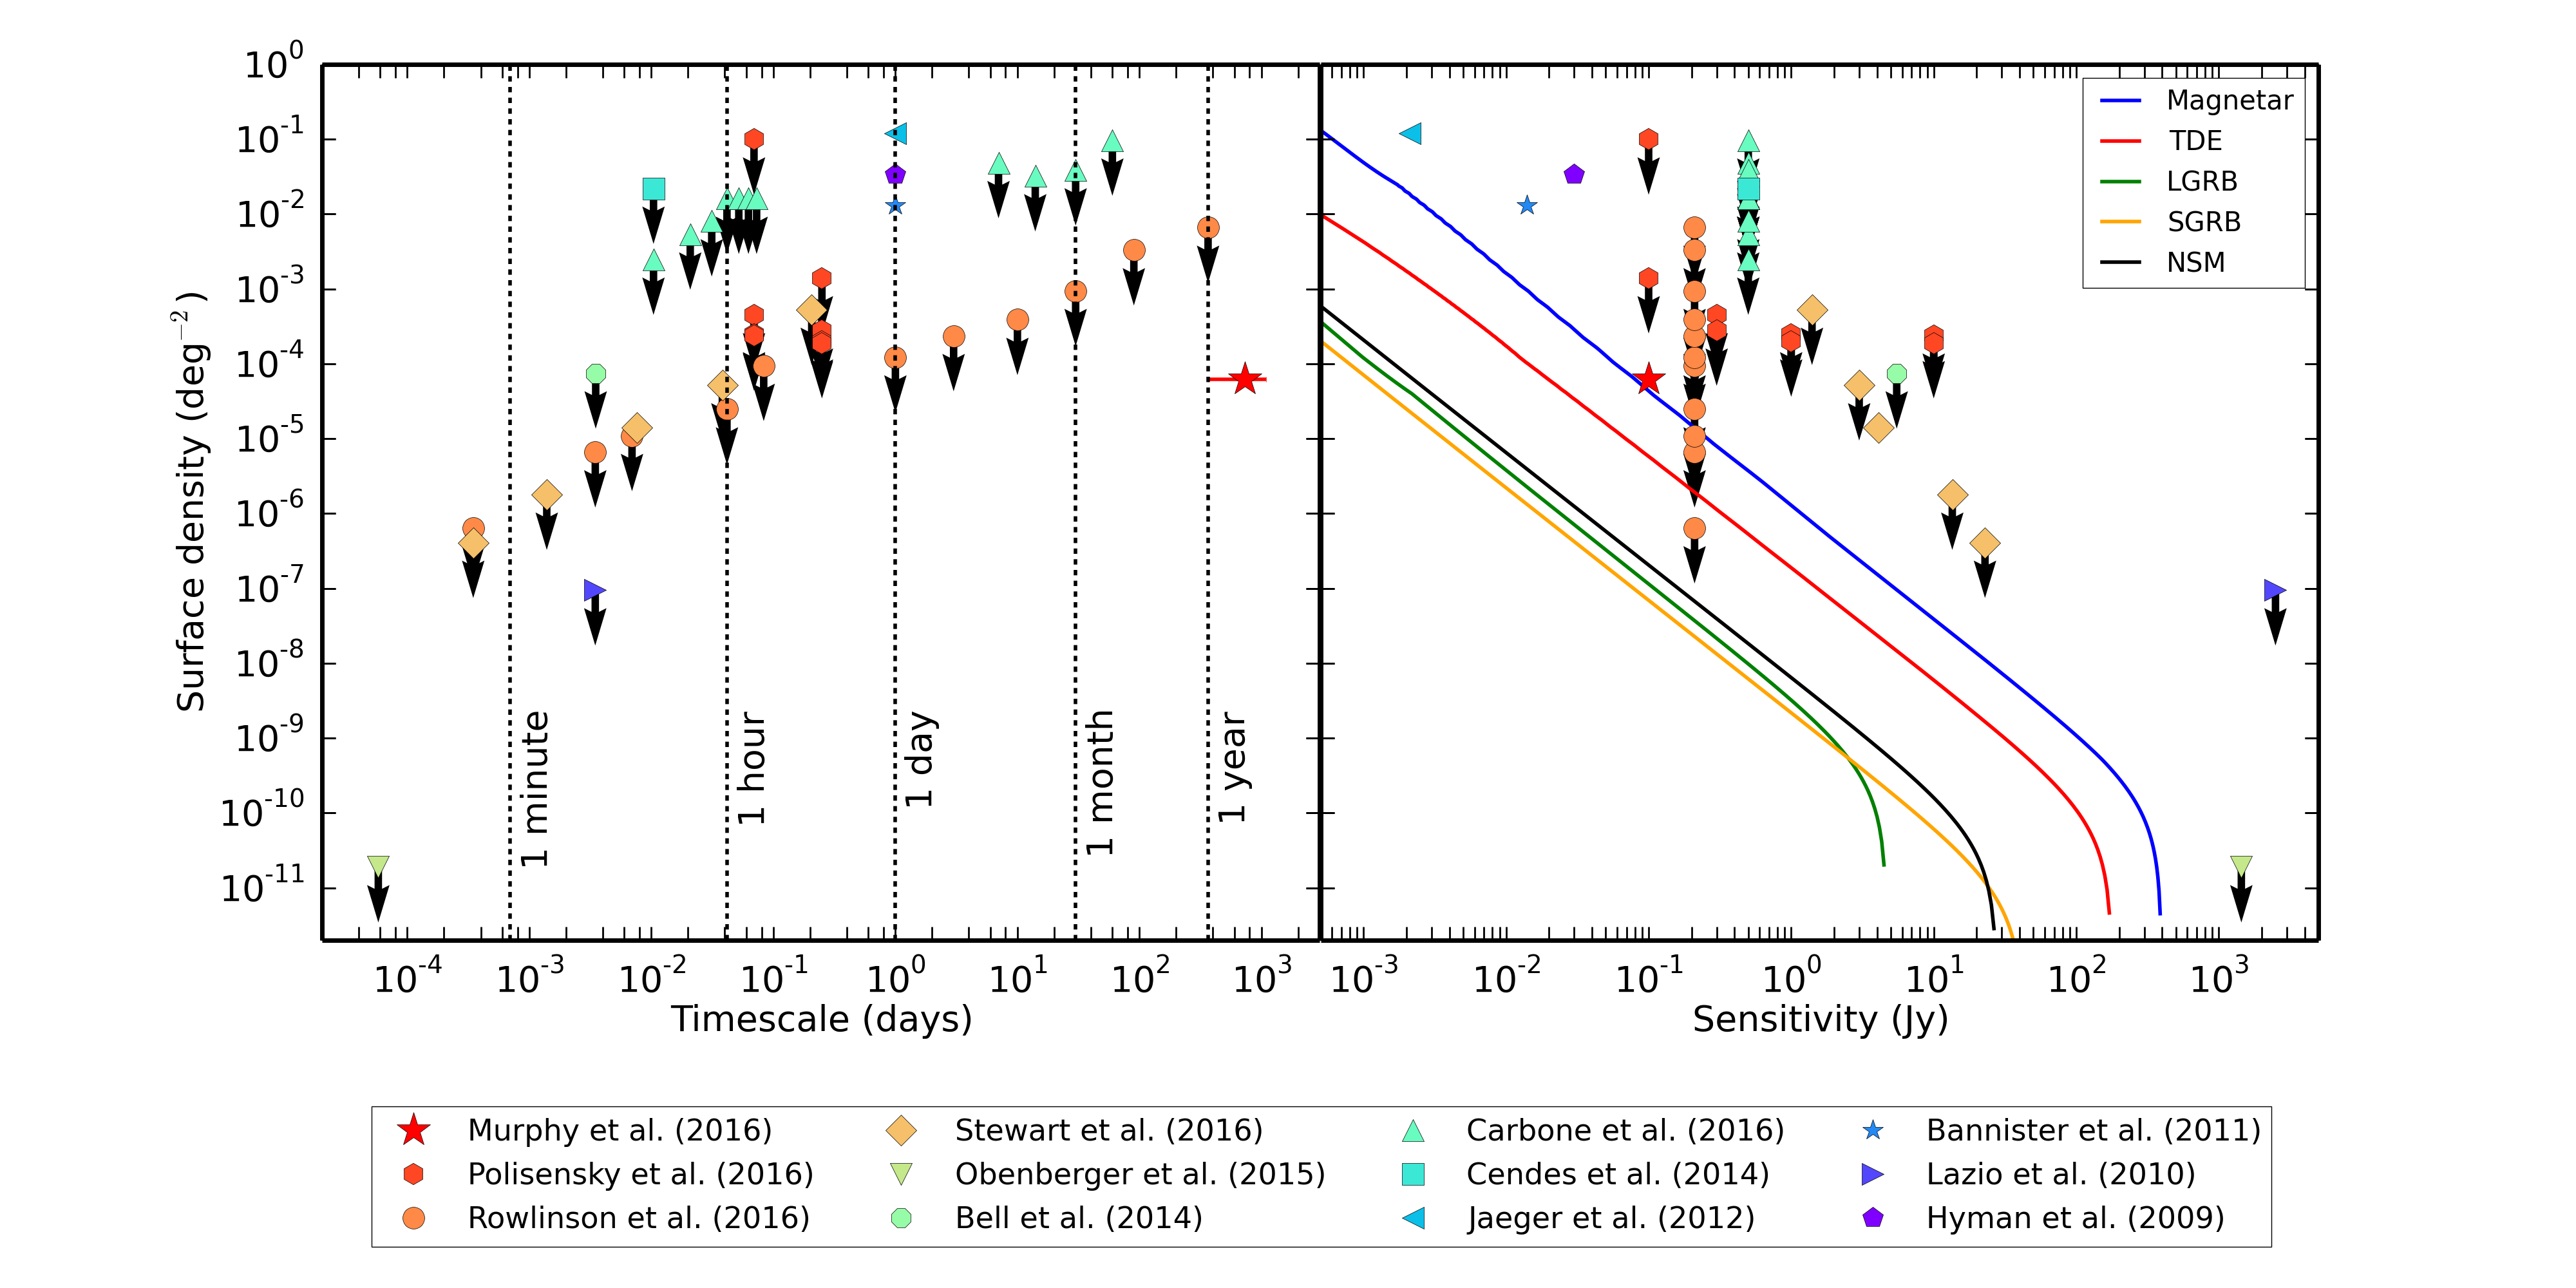
\includegraphics[width=\textwidth]{rates.png}
		\caption{These plots show the limits on the transient rate observed in radio surveys. The plot on the left shows the transient rate surface density for the timescale probed by the survey; the plot on the right shows the transient surface density for the sensitivity of the survey \citep{2017MNRAS.466.1944M}. Various transient searches around 1 GHz have probed a portion of parameter space, but there is much more that can be done. The lines for the various kinds of objects are from \citet{2015ApJ...806..224M}. These objects are magnetars, tidal disruption events (TDE), long gamma-ray burst events (LGRB), off-axis short gamma-ray burst events (SGRB), and neutron star mergers resulting in a black hole (NSM).}
		\label{murphy2017}
	\end{figure}

Figure~\ref{dario_var_lum} \citep{2015MNRAS.446.3687P} shows the kinds of objects that may be variable or transient in the radio regime. The horizontal axis shows the observing frequency multiplied by the pulse width, the latter being a proxy for the transient duration, and the vertical axis shows the spectral luminosity. Overplotted are dotted lines for different brightness temperatures: the brightness temperature is the temperature of a black body with its peak at the observing frequency\footnote{In the Rayleigh-Jeans limit, this can be represented as $I_{\nu}=\frac{2\nu^2}{c^2}kT_b$, where $T_b$ is the brightness temperature, $c$ is the speed of light, $\nu$ is the observing frequency, and $I_{\nu}$ is the intensity at a given observing frequency. See e.g. \citet{1986rpa..book.....R} for more information.}. As can be seen, different types of transients can be grouped together on this plot. On the shortest timescales are astrophysical phenomena such as fast radio bursts (FRBs), extremely short (about ten milliseconds) and bright bursts of radio emission of which the origins are still mysterious and being investigated~\citep{2021ApJS..257...59C}; and pulsars, rapidly rotating neutron stars which emit bright pulses in radio wavelengths. On longer timescales, we see phenomena like gamma-ray bursts (GRBs), mass-accreting supermassive black holes known as active galactic nuclei (AGN), supernovae from exploding stars, and X-ray binaries from stars that are in orbit with a compact object like a black hole or neutron star. 

	\begin{figure}
		\begin{center}
			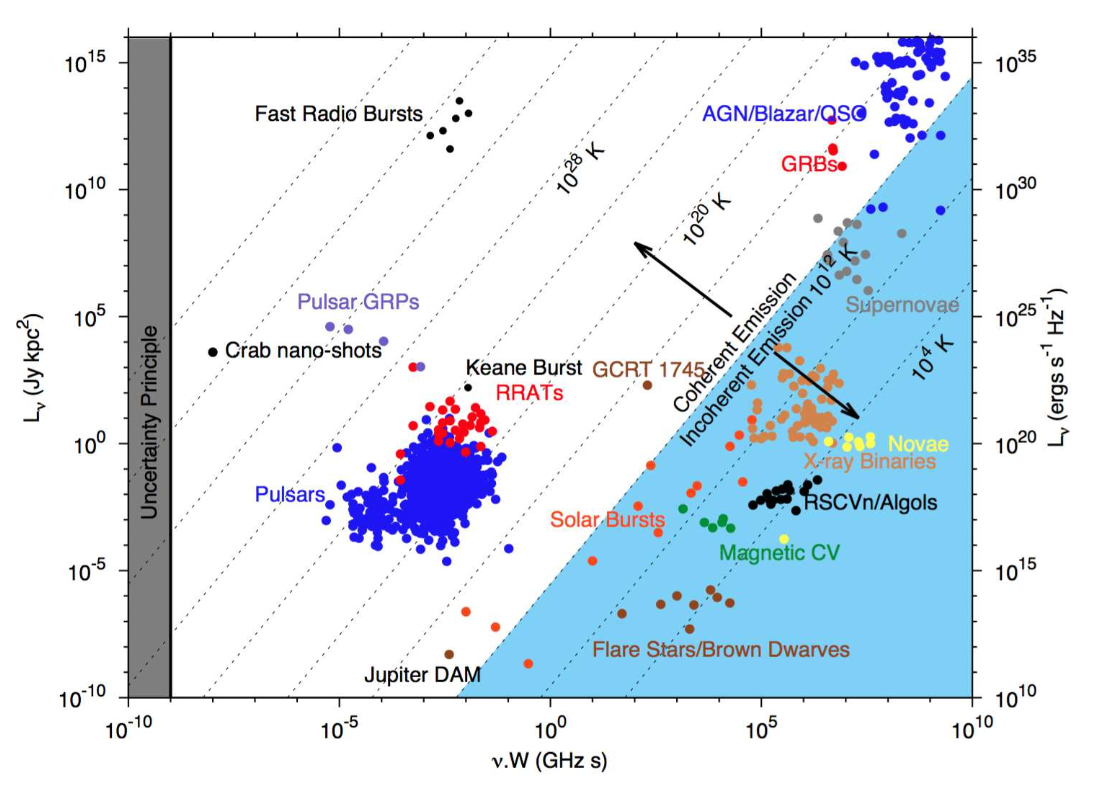
\includegraphics[width=0.8\textwidth]{dario_var_lum.png}
			\caption{From \cite{2015MNRAS.446.3687P}, spectral luminosity plotted against the observing frequency multiplied by pulse width. The diagonal lines represent different brightness temperatures.}
			\label{dario_var_lum}	
		\end{center}
	\end{figure}

Figure~\ref{dario_var_lum} \citep{2015MNRAS.446.3687P} shows that by observing at various frequencies and time scales, many different kinds of objects can be probed and perhaps some of the gaps can be filled. Furthermore, moving to lower frequencies and/or shorter duration allows for observing a broader diversity of objects, including observing coherent emission processes. This coherent emission is emission in which the properties of the electromagnetic waves are uniform, usually generated in very small and highly structured environments. At very short timescales, i.e., shorter than about 1 second, it is difficult to make a radio image, and as a result many coherent emission transients are observed using time series analysis in a high time resolution mode. 

On longer timescales it is possible to make radio images that are sensitive to the faintest of emission across multiple frequencies. This kind of detail allows for observing and characterizing synchrotron emission. Synchrotron emission is created when electrons are accelerated to relativistic speeds, producing a predictable pattern of emission over time and across the radio frequencies. This kind of emission is possible when powerful outflows and jets interact with their environments, creating shocks. By studying the exact way in which the emission behaves as a function of time and frequency, we can learn many different properties of the exact microphysics within these shocks, the global energetics, and the density and structure of the surrounding material in the environment (or medium).

 In this thesis, we focus on studying transients in radio images, which means that most of the transients we would usually expect to observe would have some sort of synchrotron emission. However, with the powerful new telescopes at our disposal we are able to make images at shorter and shorter timescales, down to even seconds. As can be seen in Figure~\ref{dario_var_lum}, this part of parameter space has very few types of known transients, and the transients that are on these short timescales include the very bright FRBs. At these short timescales, if the instantaneous sensitivity and image fidelity of the telescope is sufficient, it may be possible to detect a very bright event such as an FRB even if its duration is actually much shorter than the integration time, or the time that the radio telescope spends looking in one place. Such a detection would be possible if the transient is so bright that even after averaging out the emission over the integration time, it can still be detected. Exciting developments in radio observatories and time-domain astronomy make this an ideal moment in time to study radio transients and search for possible new types of transients.


\subsubsection{New Radio Telescopes}
Up until fairly recently, transient searches were mostly practical in the optical, X-ray or gamma-ray regime. The ability to do transient searches in radio has come with upgrades to existing facilities, such as the improved sensitivity and frequency coverage of the Karl G. Jansky Very Large Array \citep[VLA or JVLA;][]{2011ApJ...739L...1P}; and the rise of new radio facilities, such as the MeerKAT Karoo Area Telescope \citep[MeerKAT;][]{2016mks..confE...1J}, with its wide field of view and unparalleled sensitivity in its observing bands; the Low Frequency Array \citep[LOFAR;][]{2013A&A...556A...2V}, with excellent sensitivity in low radio frequencies and capabilities for resolving very small objects by using the antennae spanning the European continent; the Murchison Widefield Array \citep[MWA][]{2013PASA...30....7T}, with its excellent sensitivity at low frequencies and wide field of view; and the Australian Square Kilometer Array Precursor \citep[ASKAP;][]{2014PASA...31...41H}, with its wide field of view and excellent survey speed, just to name a few. Another crucial component to this new era of radio astronomy is the fact that computers have become advanced enough to process the immense amount of data produced by these advanced telescopes. For example, the Square Kilometer Array (SKA) \citep{2009IEEEP..97.1482D}, for which many of the aforementioned telescopes are pathfinders, is expected to need exascale-level computing power and efficiency to operate effectively, that is computing power capable of performing $10^{18}$ double precision floating point operations per second \citep{doi:10.1177/1094342014549059}. 

The upgraded VLA \citep{2011ApJ...739L...1P} began observing in 2012 and provided a vast improvement over the previous generation. It allowed for increased sensitivity, broader observing frequency bands, and vastly improved correlators and other hardware and software, allowing for better flagging and finer frequency resolution. Sensitivity increases help a great deal for transient follow-up observations. For instance, for gamma-ray bursts (GRBs), the VLA is used to follow up on detections made in other bands. Observing in the radio can provide a much clearer picture of the physics behind these events (see also the next section), and the upgrade makes that possible for a much larger sample than before (which was sensitivity limited \cite{Chandra_2012}). The VLA was a valuable resource in following up on the first electromagnetic counterpart to a gravitational wave event, GW170817, an event that was quite remarkable in the amount of new knowledge gained in several areas of physics. The peak flux of this event was at the border of what the old VLA could have observed. After this detection with the VLA, I participated in a collaboration using the VLA to follow up on gravitational wave events. This resulted in an observation for which we obtained upper limits~\citep{2019GCN.26527....1C}. In addition to following up on gravitational waves, using the VLA~\citep{2021Natur.589..207R}, I also assisted with the search for a radio counterpart to an extragalactic magnetar, a neutron star with an extremely strong magnetic field that was detected in the gamma-rays. Both of these projects are not part of the thesis presented here, since it focuses on advances made with the new MeerKAT observatory.

MeerKAT \citep{2016mks..confE...1J} is a radio interferometer in South Africa that has recently come online (summer of 2018), will be part of SKA Phase 1, and observes at mainly in the L~band (856-1711 MHz), but has recently also started observing in the UHF (544-1087 MHz) and S~bands (1750-3499 MHz). With a field of view of almost two square degrees at 1.3~GHz, and a very good image fidelity at short timescales, MeerKAT provides a unique opportunity to find transients in this observing band. It is also well suited for transient follow up since it has better sensitivity and image quality than the VLA between 1 and 2 GHz. 

In light of the excellent capabilities of MeerKAT, ThunderKAT \citep{2016mks..confE..13W} was proposed as a Large Survey Project on MeerKAT, with the goal of studying radio transients. Many important results have come from observations by the ThunderKAT collaboration, such as follow-up observations of several X-ray binaries showing jets \citep[e.g.,][]{2020NatAs...4..697B}; new transient discoveries in commensal searches, such as in~\citet{2020MNRAS.491..560D} and~\citet{2022MNRAS.513.3482A}; discoveries of variable sources and limits on transient rates such as in~\citet{2022MNRAS.517.2894R} and ~\citet{commensal1}, and many more. The wealth of deep observations taken by MeerKAT is ideal for studying and searching for radio transients like never before, even engaging citizen scientists in new ways as well~\footnote{https://www.zooniverse.org/projects/alex-andersson/bursts-from-space-meerkat/}.


\subsection{Following Up on Transients}

In addition to searching for transients, the radio regime is used to follow up on transient phenomena that have been discovered in other parts of the electromagnetic spectrum. GRBs are prime examples of transients followed up in the radio and their value to our understanding of high-energy astrophysical phenomena. 


\subsubsection{Gamma-Ray Burst Afterglows}

GRB afterglows were discovered to follow the prompt gamma-ray emission of GRBs in 1997, and the first radio afterglow emission was found for GRB~970508 \citep{1997Natur.389..261F}. GRB afterglows have a distinct synchrotron spectrum with multiple segments and characteristic frequencies \citep{1998ApJ...497L..17S,1999ApJ...523..177W}. These characteristic frequencies correspond to the minimum energy for the electron energy distribution, the synchrotron self-absorption frequency, and the cooling frequency of the most energetic electrons. The characteristic frequencies and the peak flux evolve with a certain time dependence and typically follow the Blandford-McKee solution for a relativistic blast wave at early times \citep{1976PhFl...19.1130B}. The behavior of the spectra can reveal a number of physical properties of the collimated outflow, or jet, produced in the GRB explosion, the emission processes at play, and the environment. Radio follow up is essential for getting a clear picture of the long term behavior, since the afterglow is visible in radio long after the optical and X-ray emission have disappeared; and in some cases, even until the non-relativistic phase \citep{1959sadm.book.....S, doi:10.1098/rspa.1950.0050}, such as for GRB~030329 \citep{2008A&A...480...35V}. In particular in the radio, the breaks in the synchrotron spectrum related to the minimum energy of the electron energy distribution and the self-absorption are more clearly detectable than in other bands \citep{2014PASA...31....8G}. In addition, the effects of both the forward and reverse shock are visible for a much longer time. The ability to observe the reverse shock can prove valuable for learning more about the properties of the jet itself, since the reverse shock is propagating through it \citep{2014MNRAS.444.3151V, 2013ApJ...776..119L, 2014ApJ...781...37P}. 

From multi-wavelength observations, in which the radio band plays a crucial role, we can determine physical parameters of the explosion (e.g., the energy), the environment (e.g., the ambient medium density), and the electrons and magnetic fields necessary to produce the synchrotron emission \citep{2014PASA...31....8G}. These parameters can be constrained for both long and short GRBs. Long GRBs are those which have $T_{90}>2$ seconds, where $T_{90}$ is the time during which 90\% of the gamma-ray counts are detected above background \citep{1993ApJ...413L.101K}, and short GRBs have $T_{90}<2$ seconds. Long GRBs are associated with the collapse of a massive star \citep{1998Natur.395..670G, 2003Natur.423..847H, 1993ApJ...405..273W} and short GRBs with the merger of two compact objects \citep{1989Natur.340..126E, 1992ApJ...395L..83N,2017PhRvL.119p1101A}. While radio detections of afterglows from long GRBs have been occurring with regularity for some time now, radio detections of afterglows from short GRBs are still quite rare~\citep{2015ApJ...815..102F}. It is still not completely clear why it is so challenging to detect these afterglows in radio, i.e., which physical parameters drive the radio dimness and overall dimness of short GRBs. More radio detections will be important for pinning down the causes for this.


\subsection{Structure of the Thesis}

In this thesis I will present follow-up searches of short GRBs, commensal transient searches in observations at various timescales, and detailed simulations to accurately determine transient rates from such commensal searches.

In Chapter 2 we will present accurate transient rate calculations by using Monte-Carlo simulations. In particular, we show how starting with either a real or simulated observational setup, the simulations code calculates a transient rate as a function of transient duration and peak flux. These simulations allow for replicating a wide variety of realistic scenarios including observations with varying sensitivities and durations, multiple overlapping telescope pointings, and a wide variety of light curve shapes; and this simulations toolkit is easily adaptable for a variety of different science cases.

In Chapter 3 we report on a commensal search in deep observations of short gamma-ray burst fields carried out with the MeerKAT radio telescope. These four-hour observations of eight different fields span survey lengths of weeks to months. We also carry out transient searches in time slices of the full observations, at timescales of 15 minutes and 8 seconds. We present a large number of variable sources and discuss their nature, both intrinsic to the sources as well as external, such as interstellar scintillation effects. We also place constraints on transient rates based on the transient simulations code presented in Chapter~2.

In Chapter 4 we report on another commensal transient search, using methodology established in Chapter~3, on long observations of supernova and short GRB fields. We search for transients in images with 30 minute integration times, finding several variable sources. We again explore the variability and its nature, both intrinsic and external. Also in this case, we will establish accurate upper limits on the transient rate using transient simulations. 

In Chapter 5, we use deep MeerKAT observations of seven short GRB fields to search for radio afterglow emission. We use these observations to place constraints on astrophysical parameters, in particular the efficiency of particle acceleration and emission processes, and the density of the circumburst medium. We also discuss the impact that future observatories such as the SKA will have on determining these physical parameters. Furthermore, we report the detection of possible host galaxies associated with some of these short GRBs and estimate the star formation rate, assuming the observed radio emission is indeed from star formation.

Finally, in Chapter 6, we summarize our overall results from this thesis work and provide some thoughts on future work that can be done in this area of research.




\newpage
\section{Simulating Transients for Radio Surveys}
\label{sec:transientsims}
\label{sec:sample1}

We are entering an exciting era in time-domain astronomy.  New and upgraded facilities such as the Vera C. Rubin Observatory~\citep{2019ApJ...873..111I} and Zwicky Transient Facility~\citep{2019PASP..131a8002B} in the optical, and the MeerKAT~\citep{2016mks..confE...1J} and Australian Square Kilometer Array Pathfinder (ASKAP)~\citep{2021PASA...38...54M} radio telescopes, have been finding, or are expected to find, transients and variables in images at rates that are orders of magnitude higher than ever before. This is in addition to exciting new transients found in time series data, such as the wealth of Fast Radio Bursts (FRBs) found using the Canadian Hydrogen Intensity Mapping Experiment (CHIME)~\citep{2019Natur.566..235C}. 

Many transients are discovered in blind searches, found by examining large portions of the sky for new sources or known sources that display significant flux changes. There are also transients found in a targeted way, such as those associated with gravitational wave events~\citep{2017PhRvL.119p1101A,2017Natur.551...71T,2018ApJ...868L..11M}, gamma ray bursts~\citep{1997Natur.389..261F,2018MNRAS.473.1512A}, tidal disruption events~\citep{2011Sci...333..199L,2016Sci...351...62V}, and outbursts from X-ray binaries~\citep{2004MNRAS.355.1105F,2017MNRAS.469.3141T}. Considering that transients can be found in both blind and targeted searches brings up important questions: if we are doing a targeted transient search, what is the chance that a detection may be a different transient source that happens to be in the same area of the sky, even within the same uncertainty region of the transient of interest? How many transients of a certain type or with a specific light curve shape would we expect to find in a given survey? Finding the answers to these questions is important for a variety of applications in time-domain astronomy and requires calculating transient rates with high accuracy. 

The most straightforward approach to calculating a transient rate is to use the Poisson distribution to find a rate given the number of detections in a survey, but there are shortcomings in this simplified approach~\citep{2016MNRAS.459.3161C}. This transient rate does not account for a number of important factors such as the relative timescales of the transients and the observations, and some of the confounding observational effects such as gaps within an observation or a survey. In addition, it does not account for the distribution of sensitivities present in the observations of a real survey. These effects can be partly mitigated in an analytical approach~\citep{2016MNRAS.459.3161C}, but Monte-Carlo simulations provide a way to more easily account for the issues presented by real observations and surveys in transient rate calculations~\citep{2017MNRAS.465.4106C}. 

\citet{2017MNRAS.465.4106C} examined two light curve shapes: the tophat light curve, a light curve that instantaneously rises to its peak flux and at some point in time instantaneously decays; and the fast rise exponential decay (FRED) light curve, a light curve that instantaneously rises to its peak flux and exponentially decays thereafter. The differences between the resulting transient rates from these two light curve shapes indicate how the wide variety of real light curves can affect transient rate calculations. This is in addition to the previously mentioned observational effects that should be accounted for. 

Observational radio surveys present a number of challenges for computing transient rates. Although radio observations can be calibrated using a sky model, many radio observations require the use of calibrator fields that need to be observed at certain time intervals before, after, and during an observation of a science target field. This means that the telescope does not continuously point at a target for an entire observation. Often when using a calibrator source, a radio observation would be broken down into observing a very bright, well-known source to calibrate the bandpass, followed by alternately observing a bright source close to the target for gain calibration and the science target. This means that the time on target is less than the total observing time, and that there are gaps in the target observations. This also means that there is the possibility of searching calibrator fields for transients \citep{2011ApJ...728L..14B}. Furthermore, typical radio observations can be broken down into shorter timescales for imaging. In addition, in order to explore a wider field of view, a survey may consist of multiple adjacent pointings on the sky with some degree of overlap between pointings. These pointings may have different limits on transient rates due to differing observing cadences, and the overlap regions will provide different transient rates as well.

The goal of this work is to calculate transient rates while accounting for the aforementioned features and complexities of radio surveys. Corrections for observational effects such as gaps in observations, systematic errors in flux measurements, different kinds of transient light curves, multiple overlapping pointings, and a distribution of observational sensitivities are accounted for. Mitigating all the aforementioned effects makes the transient rate calculations more accurate. In addition, the publicly available simulations code is relatively simple in its use, has Python 3 support, and is designed for modularity so that the user can easily add new items such as other light curve shapes than those already provided.

In the Design section, we will go into detail on how the code is written and its features implemented. We will in the Results and Discussion section present and discuss results from several example radio surveys illustrating the various features. In the Performance section, we will look at the computational performance of the simulations code. In the Future Applications section we will discuss the ways in which this code can be expanded in the future, and we draw conclusions in the final section. 



\subsection{Design}
\label{design}
\subsubsection{Language and Libraries}
The code was written in Python\footnote{http://www.python.org} and designed for its most up-to-date versions ($>3.6$). It uses several libraries: Astropy~\citep{2013A&A...558A..33A} to provide accurate angular source separation calculations and any necessary coordinate system changes; Scipy~\citep{2020NatMe..17..261V} for a few special mathematical functions; Bitarray\footnote{https://github.com/ilanschnell/bitarray} for storing large amounts of information efficiently; tqdm\footnote{https://tqdm.github.io} for easy-to-use progress bars; and Numpy\footnote{https://numpy.org/} for the vast majority of the numerical computations. In addition, the script to assist with creating input files uses Common Astronomy Software Applications (CASA)~\citep{2007ASPC..376..127M} to read and extract metadata from radio measurement sets. 
% Is it possible that I'm listing to many libraries/details here? 

By using an interpreted language that allows for the use of classes, the code is easy to modify or extend for different use cases, or to increase accuracy. Adding new light curves can be done by creating a Python file with the name of the light curve and a class with the essential information. Using Numpy partially makes up for Python's lack of speed compared to a compiled language such as C. The information on whether a simulated source is detected is stored and written using bit arrays, in order to reduce memory usage so that these computations can be performed on a regular desktop or laptop. 

\subsubsection{Input}
In order to accurately simulate transient rates, it is necessary to provide detailed information on the survey that will be simulated. This information includes observation times, pointings, field of view, sensitivity, and any gaps in the observations. This information is either supplied by the user as a comma-separated values (CSV) file or it can be generated using a separate script that extracts information from the metadata in the measurement sets of the survey observations.

In addition, the simulations code base contains a configuration file with settings that can be adjusted depending on the use case. These settings include items such as number of transients to simulate, number of transient detections in the survey, flux and duration ranges to simulate, detection threshold, light curve type, confidence level, output filename, and options for simulating a survey such as number of observations, sensitivity, mean and standard deviation of simulated normally-distributed error in sensitivity, interval between observations, and the duration of the observations. The light curve type can be any of the included ones or a new light curve created by the user. 


%%%%%%% NEW FIGURE 
\begin{figure}
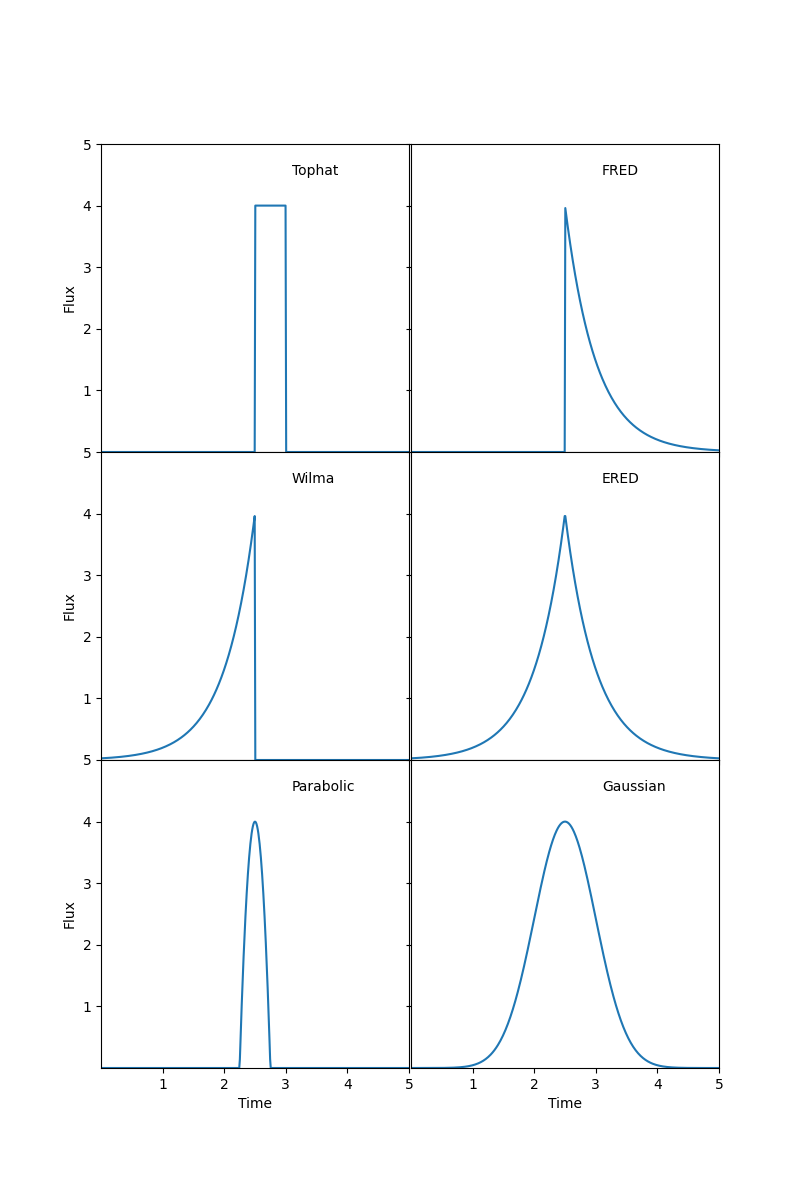
\includegraphics[width=0.8\columnwidth]{multilcexample.png}
\caption{Examples of all light curve shapes included in the simulations in this paper, plotted using arbitrary units of time and flux.}
\label{multilc}
 \end{figure}
 %%%%%%%%
\subsubsection{Light Curves}
In Figure~\ref{multilc} we show the light curves included in the simulations, which are the tophat, fast rise exponential decay (FRED), exponential rise fast decay (Wilma), exponential rise exponential decay (ERED), Gaussian, and parabola. The tophat light curve is defined to have an instantaneous rise to the peak flux, followed at some point in time by an instantaneous decay. This light curve represents the classic case of a transient that turns on and off, and the simplest form of transient light curves. The FRED light curve instantaneously rises to the peak flux and exponentially decays. This light curve is commonly observed in a variety of X-ray and gamma-ray transients. The Wilma is simply the time reversed FRED: it exponentially rises to the peak flux and then instantaneously decays. Including the ERED light curve is a convenient way to introduce the simplest form of light curve with no definite start or end. The ERED is such a light curve that is formed by putting the previous two together: it exponentially rises to a peak flux and then exponentially decays. The Gaussian is a light curve that has the shape of a Gaussian function with the mean being located at the peak flux and the duration given by the standard deviation. Similar light curves can be seen arising from, for example, binary systems and magnetar bursts.  The parabolic light curve is a concave down parabola that reaches the peak flux at the vertex and the duration being the range of time in which the flux is positive; its inclusion provides an example of a light curve with a definite duration but with a profile that rises and falls below the peak flux in a symmetric way (i.e., one step more complex than the tophat). More details about these light curves, including their mathematical definitions, can be found in the appendix to this chapter.

For a given radio survey, the simulated light curve has implications on the part of parameter space that the survey probes. One of the clearest ways to examine these implications is by looking at probability contour plots. Figures~\ref{tophat}-\ref{fred} show the probability contours for example light curves included in the simulations code. The horizontal axis shows the characteristic duration of the transient, which is defined slightly differently for each light curve shape: the tophat and parabolic light curves' characteristic duration is the duration that the transient's flux is non-zero; the characteristic duration for the Gaussian is the standard deviation; and the duration of the FRED, Wilma, and ERED light curves is the e-folding time. The vertical axis shows the characteristic flux, which is the peak flux for all light curves that are currently implemented (but could vary for more exotic light curve shapes). The color legend shows the probability of detecting a source as a transient at a given duration and flux. Note that a source that is detected in every observation would not be a transient. A probability of 1 means that the survey detects every transient source at the particular flux and duration. Note how the region where the transient is always detected changes for the different light curve shapes. The reason for some of these differences is discussed in detail in the Light Curves section.

 \begin{figure}
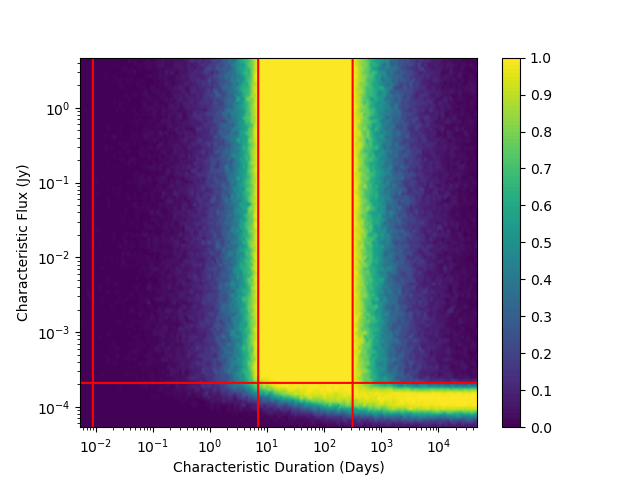
\includegraphics[width=\columnwidth]{tophat.png}
\caption{Probability contours for the tophat light curve. The leftmost vertical line marks the shortest observation in the survey, the middle line corresponds to length of the longest gap between observations, and the rightmost line corresponds to approximately the length of the survey itself. The horizontal line is a line marking the flux value that is greater than 99\% of the flux values of the false transient sources.}
\label{tophat}
 \end{figure} \begin{figure}
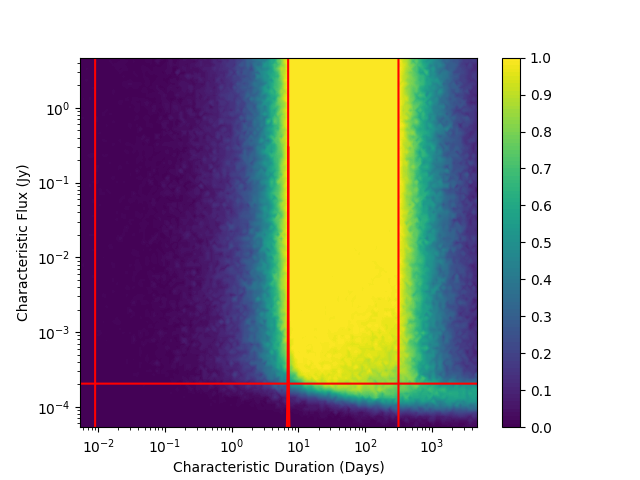
\includegraphics[width=\columnwidth]{parabolic.png}
\caption{Probability contours for the parabolic light curve. The meaning of the horizontal and vertical lines is the same as in Figure~\ref{tophat}.}
\label{parabolic}
 \end{figure} \begin{figure}
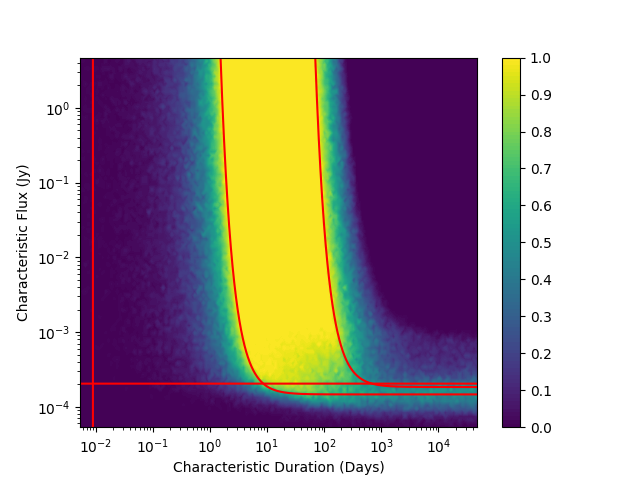
\includegraphics[width=\columnwidth]{gaussian.png}
\caption{Probability contours for the Gaussian light curve. The leftmost vertical line marks the shortest observation in the survey, the curve in the middle marks a boundary in the duration of sources to the left of which these sources can fall in the longest gap between observations and go undetected in any observations, and the rightmost curve is a boundary to the right of which sources can be detected as a constant source by being detected in every observation. The meaning of the horizontal line is the same as in Figure~\ref{tophat}.}
\label{gaussian}
 \end{figure}\begin{figure}
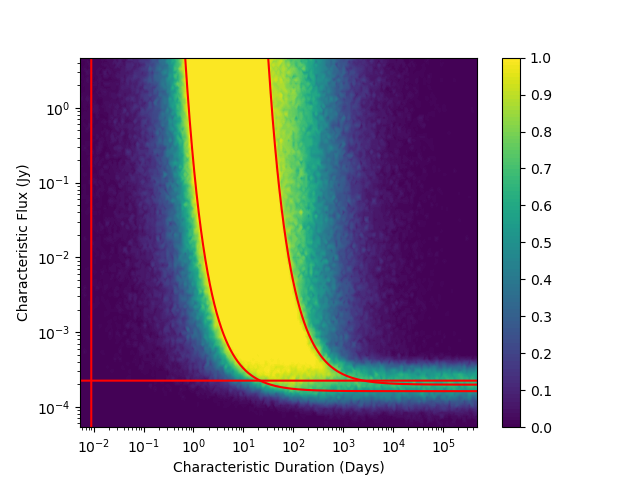
\includegraphics[width=\columnwidth]{fred.png}
\caption{Probability contours for the FRED light curve. The meaning of the horizontal and vertical lines is the same as in Figure~\ref{gaussian}.}
\label{fred}
 \end{figure}
 

\subsubsection{Main Detection Algorithm}

In the transient simulations, a large number of sources need to be generated based on the user's settings. Parameters such as the source flux, duration, and the start, end or critical time (depending on the light curve type) are generated in a uniformly random fashion in log10 space via the random number generator in Numpy. 

The main detection algorithm tests whether or not the simulated sources will be detected in the observations. For this step, the code iterates over each observation, calculating the integrated flux for all the simulated sources, and testing if these integrated fluxes are greater than the sensitivity of the observation multiplied by a user-specified detection threshold. After this detection step, the sources that are detected in every observation are removed from the detection list, since they are constant sources and not transients. 

The number of detected transient sources together with the number of simulated sources are used to generate probabilities of detection for each flux and duration bin. Assuming that transients are distributed as a Poisson distribution, the probabilities are used to calculate limits on transient surface densities and rates. In the case of no transient detections in a survey, the Poisson probability mass function can be inverted to give an upper limit. In case of transient detections in the survey, the code uses the $\chi^2$ distribution \citep[for a review see][]{12005udd3.inbook.....JKK} to calculate the upper and lower limits on the transients rates, by inputting the user-provided confidence level and the number of transient detections in the survey. 

%% Poisson explainer HERE 

% I considered doing a section on ``incorporating detections'' here, but I decided not to because it would be only one sentence: ``Finding limits on transient rates in the case of purely non-detections is straightforward: one can merely invert the Poisson Distribution (if one assumes transients to be distributed thusly); however, finding upper and lower limits is slightly more complicated: one has to use the inverse incomplete gamma function as shown in~/ref{whatever textbook}.''

\subsubsection{Gaps}

An important ingredient in calculating transient rates accurately is taking into account gaps of varying sizes during observations and surveys. These gaps may exist for a variety of reasons. In the case of radio observations, a long observation on a particular source has to be broken up into scans that are briefly interrupted by observations of a calibrator source. For measuring the flux of a particular source of interest, these gaps are usually unimportant, but for the purposes of calculating transient rates, especially transient rates in a regime where the transients may be shorter than the size of the gaps, it is important to account for these gaps. 

Gaps are accounted for in the simulations code base by specifying a gaps file. This file contains all the sub-observations, also known as scans, that make up the full length observation. By running the simulations over the scans, and averaging together the measured flux in each scan, we are able to account for realistic gaps in observations. By correcting for these gaps, we are able to account for multiple different timescales and different sensitivities present in the same survey in an accurate way that would not be possible, or at least very challenging, to do in an analytic fashion \citep{2016MNRAS.459.3161C}.




\subsubsection{False Detections}
False transient detections is an issue that affects real transient searches and should therefore be included in transient simulations. When an astronomical source is close to the detection threshold, any small amount of measurement error, either statistical or systematic, can change it from a detection to a non-detection or vise-versa. Since this can be true for every observation in the survey, there can exist a fairly wide distribution of false transient detections, governed by the sensitivities of the observations. These sources will be flagged as transients, which is an issue because they are not real transients but merely faint sources of constant flux. Therefore, it is necessary to find a way to eliminate these sources from consideration as transients. 

In order to solve this problem, a second run through the detection algorithm is performed using sources with tophat light curves along with duration and start times that ensure that they ought to be constant sources. After the false detections of these constant sources are calculated, the number of sources detected are counted from the minimum flux simulated until 99\% of the falsely detected sources are accounted for. At the flux level where 99\% is reached, we define this to be the false detection limit. This is shown in all of the probability contour plots, such as in figures~\ref{tophat}-\ref{fred}, and transient rate plots as a horizontal line. 



\subsubsection{Multiple Pointings}
Real surveys can involve multiple pointings that overlap, resulting in an uneven probing of the sky. This creates opportunities and challenges for determining transient rates in these regions of the sky, due to the differences in timescales and observed area. 
In order to account for this, the simulations accurately calculate the area of each region on the sky, and then determine the transient rates for each region on the sky. This is currently implemented for a maximum of three overlapping pointings with possibly varying observing timescales and cadences, but an expansion of this is easily doable. 

% The journal wants the figures separately
\begin{figure}
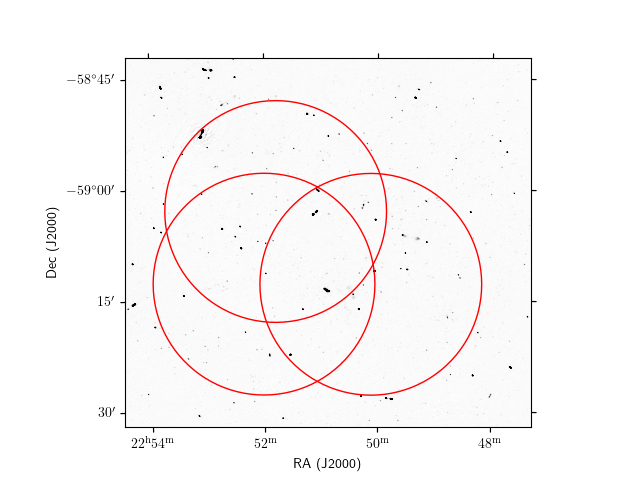
\includegraphics[width=\columnwidth]{Figure_1_blank.png}
\caption{An example of three overlapping pointings with red circles representing three different telescope pointings that overlap}
\label{threepointings}
 \end{figure}

Figure \ref{threepointings} shows a simulated example of three overlapping pointings. Each red circle represents a pointing of the telescope. It can be seen that there are also three double overlap regions and one triple overlap region. For each of these regions, the transient rates will be different due to the differences in observing cadence and time. 



\subsection{Results and Discussion}\label{sec:results1}

\subsubsection{A Realistic Survey}

\begin{figure}
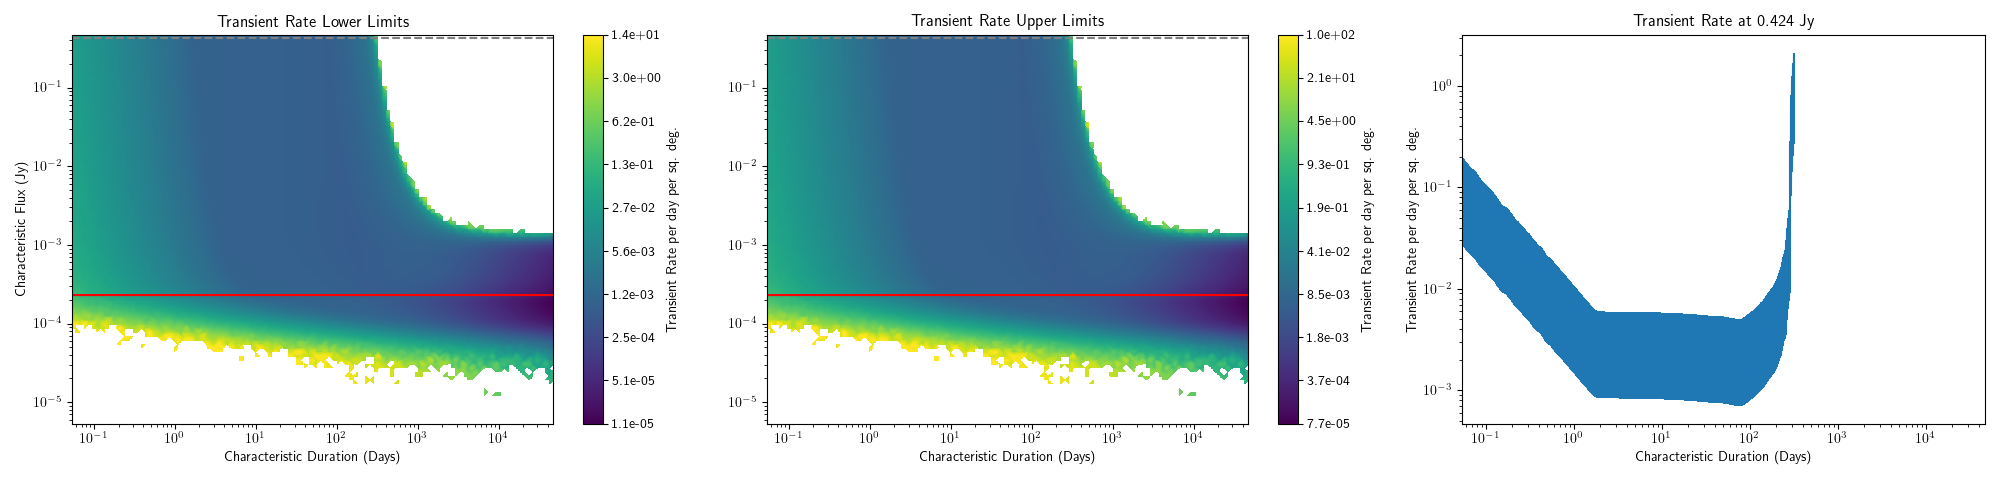
\includegraphics[width=\columnwidth]{figure2.png}
\caption{Lower limits (left) and upper limits (middle) on transient rate for a realistic survey setup. The red line indicates the false detection limit. The plot on the right shows the limits on the transient rate at 0.424 Jy, which is marked on the two plots to the left with a dashed line at the very top of the plots.}
\label{realscen}
 \end{figure}

For the purpose of demonstrating the capabilities of the transient simulations code, a survey setup similar to that in \citet{10.1093/mnras/stz3027} is used: 46 weekly observations of 13 minutes in duration, with the rms noise of the observations being varied as a Gaussian with mean 35 $\mu$Jy and standard deviation 5 $\mu$Jy and a detection threshold of $5\sigma$. Given that transients were detected in \citet{10.1093/mnras/stz3027} , we also demonstrate the ability of the simulations code to calculate transient rates based on detections. Assuming Poisson statistics, one can calculate the upper and lower limits on the transient rate, as explained in the previous section. In the configuration for this simulations run, two transient detections are used as input to calculate the rates along with a 95\% confidence interval. The light curve type used for this example is the Gaussian.

Figure \ref{realscen} shows the results of these simulations. The left-side plot shows the lower limits on the transient rate, the middle plot shows the upper limits on the transient rate, and the plot on the right shows the example of transient rate limits at 0.424 Jy as a function of transient duration. The horizontal red lines indicate the 99\% false detection rate. These plots show the transient rate limits: we can see that at 0.424 Jy and around a transient duration of 10 days, the transient rate is between $7\times10^{-4}$ and $5\times10^{-3}$ transients per day per square degree. 

\subsubsection{Light Curves}\label{lcdiscussion}
Figures~\ref{tophat}-\ref{fred} show the probability contours for the tophat, parabolic, Gaussian, and FRED light curves. These probabilities are the ratios of the detections to total simulated sources for each duration and flux bin. Each plot has a region of parameter space where all of the transients are detected. As shown by \citet{2017MNRAS.465.4106C}, in the tophat case this is bounded on the left by the duration of the longest gap between consecutive observations. The boundary on the right corresponds to the longest possible duration transient that will still be considered a transient and not a constant source. In other words, this duration is slightly less than the length of the entire survey, since a transient of this length would be detected in every observation except for one.  For the FRED, Gaussian, Wilma, and ERED light curves, we observe that the boundaries around this same region are curves. In the appendix, we go into detail on finding the equations for these curves. 

Examining the probability contours for the parabolic light curve in Figure~\ref{parabolic} shows a plot that looks closer to the tophat than the other light curves due to the vertical boundaries on the region where the probability is equal to 1. While this may seem counter-intuitive, a similarity between the parabolic and tophat light curve is that they both have a fixed start and stop time at which the flux drops to zero. All the other example light curves approach but never reach zero. For this reason, we use a value to characterize the duration such as the e-folding time for the FRED, or the standard deviation in the case of the Gaussian light curve. Using these values to characterize the duration is what causes the difference in these probability contours. As an example, for the FRED light curve, if the transient has a low flux compared to the sensitivity of the observations, then the duration of the transient that would be detected might be something closer to its e-folding time. In contrast, a very bright transient would be detected well past its e-folding time. This is the reason why these light curves seem to curve away to the left as flux increases in these probability contour plots: the actual duration that is detected in the survey becomes longer. If we were able to define the duration of the transient by the duration that is actually detectable in the survey, then we could make all of the probability contour plots have the kinds of vertical boundaries that we see in the tophat and parabolic light curves. However, defining the durations this way, would make the simulations much more computationally and mathematically complex to the extent that it makes this prohibitive. 

\subsubsection{False Detections}  \label{fddiscussion}
Figure~\ref{fig9} shows an example of a survey with a large number of false detections of transients. This can happen when including images that are grouped around very different sensitivity scales. In the example shown here, the survey included observations on three very different time scales and sensitivities: 4 hour observations with an rms noise of around $9~\mu$Jy; 15 minute observations with an rms noise of around $30~\mu$Jy; and 8 second observations with a noise around $350~\mu$Jy. Including all of these images in one run of the simulations creates many false detections. In this example, it is better to run simulations of these three different time and sensitivity scales separately. In figures~\ref{sample4hr}-\ref{sampleint}, the probability contours for the three different timescales are shown separately. From these plots, we can clearly see that the false detection limit is much lower on two of the three timescales and a little higher on the shortest timescale. 



\subsubsection{Gaps} \label{Gaps}
In order to demonstrate the capability of including observations with gaps, an observation file was created with weekly 4 hour observations (instead of 13 minutes), containing gaps within the weekly observation, and a total survey duration of 46 weeks (as in the previous example). The gaps were typical for a target-gain calibration loop in radio observations: 5 minutes on a calibrator field followed by 15 minutes on a science target field. The noise in the 15-minute scans was simulated like before, with a mean of 35 $\mu$Jy and a standard deviation of 5 $\mu$Jy in the target observations. For the full four hour observations, the noise was scaled as $1/\sqrt{time}$ and simulated as a Gaussian with a mean of 8 $\mu$Jy and a standard deviation of 1 $\mu$Jy. Due to the nature of having a bright calibrator source in a field, the noise for the calibrator observations was higher than would be suggested by scaling by $1/\sqrt{time}$. The noise of the 5 minute scans of the calibrator observation was simulated to be 100 $\mu$Jy with a standard deviation of 15 $\mu$Jy. The noise of the combined image of the calibrator scans was simulated to be 25 $\mu$Jy with a standard deviation of 4 $\mu$Jy. For this example we assume that there are no detected transients in this simulated survey.

\begin{figure}
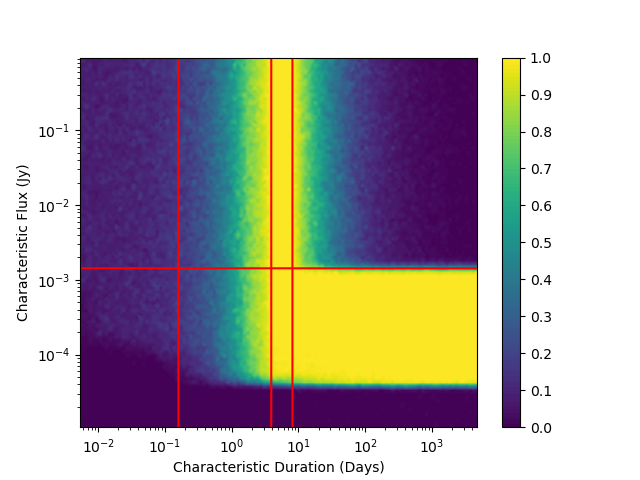
\includegraphics[width=\columnwidth]{figure9.png}
\caption{Probability contours for a tophat light curve in a survey with very different observation sensitivities (see main text for details).}
\label{fig9}
 \end{figure}
 \begin{figure}
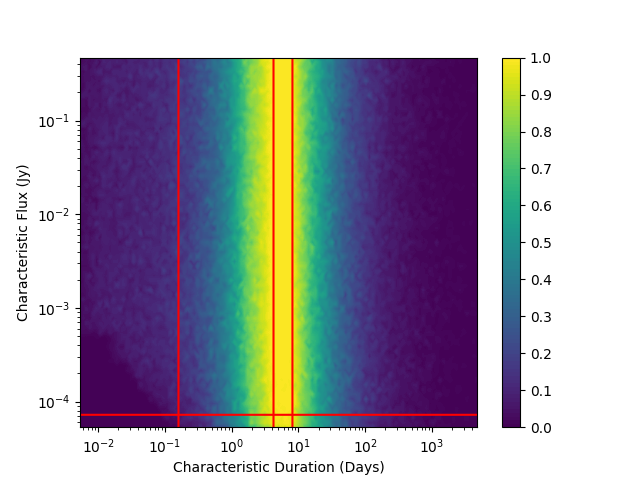
\includegraphics[width=\columnwidth]{sample4hr.png}
\caption{Probability contours for a tophat light curve in a survey with only 4 hour observations at an rms noise of around $9~\mu$Jy.}
\label{sample4hr}
 \end{figure}
 \begin{figure}
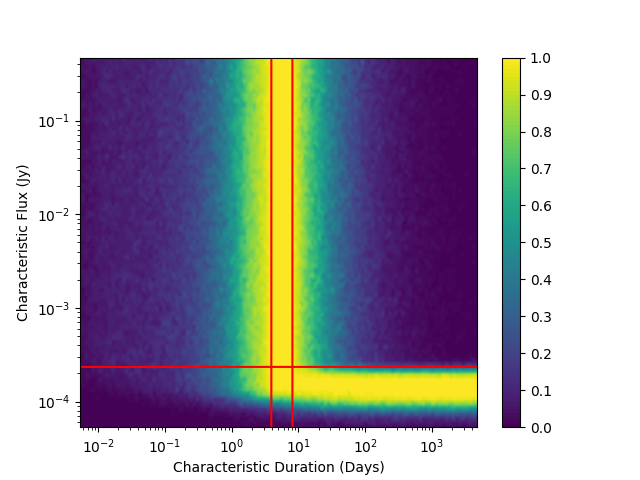
\includegraphics[width=\columnwidth]{samplescan.png}
\caption{Probability contours for a tophat light curve in a survey with only 15 minute observations at an rms noise of around $30~\mu$Jy.}
\label{samplescan}
 \end{figure}
 \begin{figure}
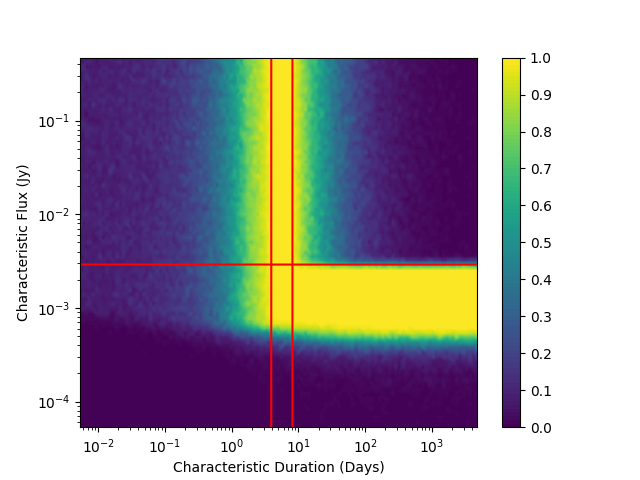
\includegraphics[width=\columnwidth]{sampleint.png}
\caption{Probability contours for a tophat light curve in a survey with only 8 second observations at an rms noise of around $350~\mu$Jy.}
\label{sampleint}
 \end{figure}

Using these simulations, we can show how accounting for gaps results in more accurate transient rate calculations. This is particularly important on timescales close to the length of the gap itself. In order to test the gaps algorithm, three observational scenarios were used: the calibrator field with 15 minute gaps, the target field with 5 minute gaps, and a full four hour observation with no gaps. These scenarios provide a comparison between different extremes of gaps in observations. These simulations were done with both tophat and FRED light curves. Figures \ref{fig3}-\ref{fig8} show the results of these scenarios. Figures~\ref{fig3} and~\ref{fig4} show upper limits on transient rates in the color legend, with transient duration on the horizontal axis and characteristic flux on the vertical axis. Figure~\ref{fig3} is for a tophat light curve and Figure~\ref{fig4} is for a FRED light curve. The three plots in each figure show the difference in transient rates when not accounting for gaps in a weekly survey with 4 hour observations (top), when accounting for 5 minute gaps in a 4 hour science target observation (middle), and when accounting for 15 minute gaps in calibrator observations (bottom). 

In figures~\ref{fig3} and~\ref{fig4} we can see a diagonal trend at the shortest durations below which there are no colored contours. This boundary marks the transients that are shortest in duration and lowest in flux to possibly be detected. It is a diagonal because it is the fluence that determines if a transient is detected \citep{2017MNRAS.465.4106C}; and in the FRED case, for short durations the integrated flux becomes identical to the tophat case. The blank space in the bottom left of the plots represents the region of transient parameter space that cannot be probed by the simulated survey. The red vertical lines on these plots mark 5 minutes, the length of the gaps in the target observations. 

Differences in the transient rate are small and difficult to distinguish between the target gap and no gap plots in figures~\ref{fig3} and~\ref{fig4}. The calibrator gap shows a bit of a departure from the others: examining closely reveals a slightly different trend to the left of the red line for both light curves. This departure from the case of having no gaps or the case of a smaller gap only shows in the part of parameter space that has the smallest duration transients. When transients are longer in duration, they are not likely to fall in the gaps and are more likely to be detected in an observation. 

Figures~\ref{fig5} through~\ref{fig8} show the differences between the different gaps in a different way. Figures~\ref{fig5} and~\ref{fig6} show the transient rates from Figures~\ref{fig3} and~\ref{fig4} on the vertical axis at a constant flux of 0.464 Jy. Figures~\ref{fig7} and~\ref{fig8} show the percent difference in transient rate between the gaps and no gaps cases. The top panel of Figures~\ref{fig7} and~\ref{fig8} shows the difference between the target gap and no gap cases, and the bottom plot shows the difference between the calibrator gap and no gap cases. As we can see there is an appreciable difference when accounting for 5 minute gaps in a target observation, and a significant difference of nearly 300\% when accounting for 15 minute gaps in the calibrator observation.

\begin{figure}
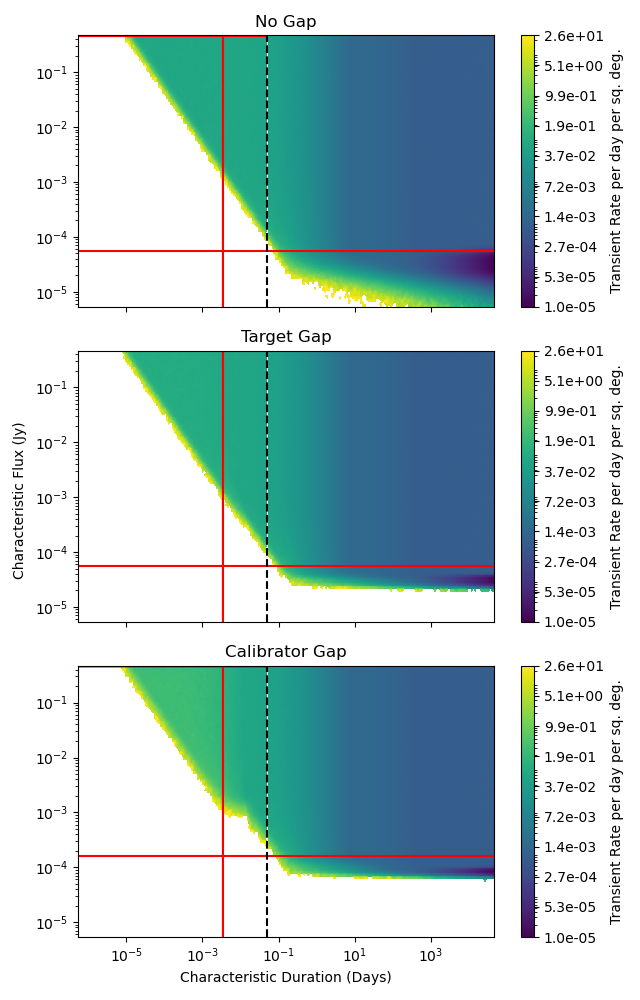
\includegraphics[width=0.75\columnwidth]{figure3.png}
\caption{Upper limits on transient rate for transients with a tophat light curve in a survey with 4 hour observations with no gaps (top), 5-minute gaps in between 15-minute observations (middle), and 15-minute gaps in between 5-minute observations (bottom); see main text for sensitivities of observations. The dashed black line marks where two different simulations were combined into a single plot. The vertical red line indicates 5 minutes, and the horizontal red line indicates the false detection limit.}
\label{fig3}
 \end{figure}
 
 \begin{figure}
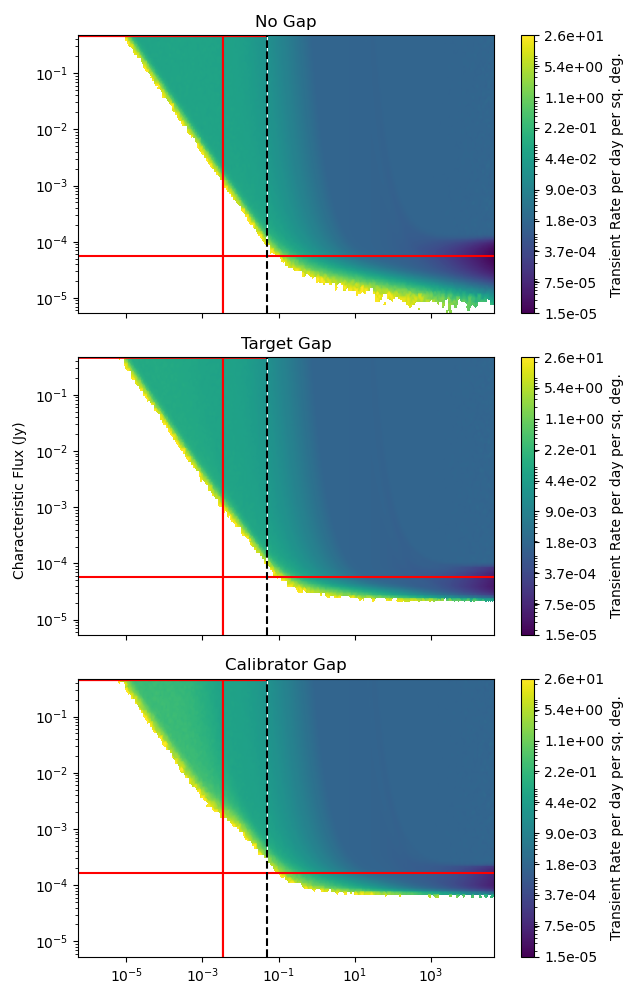
\includegraphics[width=0.75\columnwidth]{figure4.png}
\caption{Upper limits on transient rate for transients with a FRED light curve in a survey with 4 hour observations with no gaps (top), 5-minute gaps in between 15-minute observations (middle), and 15-minute gaps in between 5-minute observations (bottom); see main text for sensitivities of observations. The dashed black line marks where two different simulations were combined into a single plot. The vertical red line indicates 5 minutes, and the horizontal red line indicates the false detection limit.}
\label{fig4}
 \end{figure}
 
 \begin{figure}
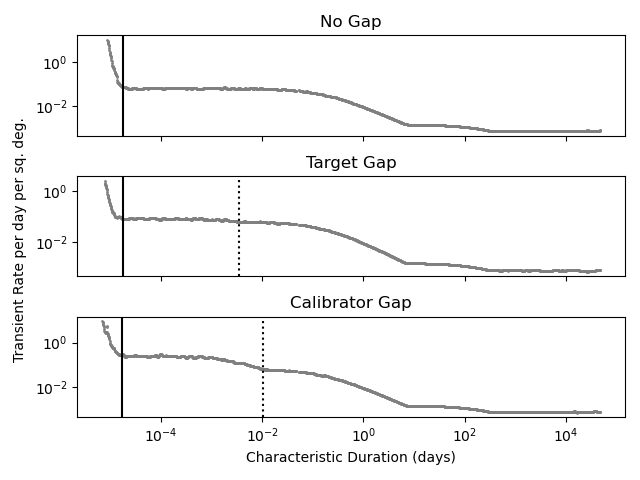
\includegraphics[width=0.75\columnwidth]{figure5.png}
\caption{Upper limits on transient rates for transients with a tophat light curve in a survey with 4 hour observations with no gaps (top), 5-minute gaps in between 15-minute observations (middle), and 15-minute gaps in between 5-minute observations (bottom), for transients with a peak flux of 0.464 Jy.}
\label{fig5}
 \end{figure}
 
 \begin{figure}
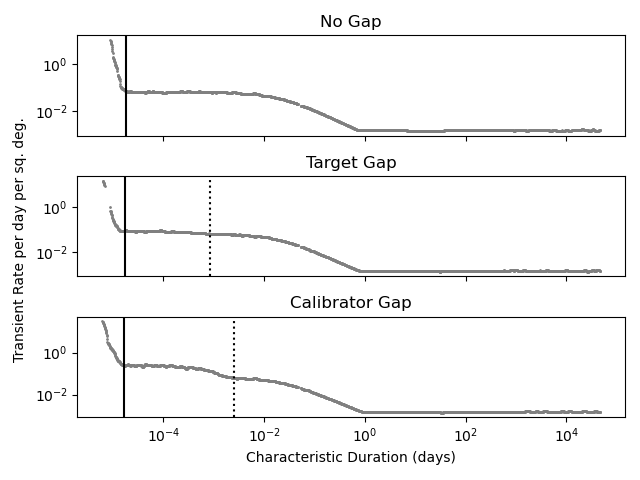
\includegraphics[width=0.75\columnwidth]{figure6.png}
\caption{Upper limits on transient rates for transients with a FRED light curve in a survey with 4 hour observations with no gaps (top), 5-minute gaps in between 15-minute observations (middle), and 15-minute gaps in between 5-minute observations (bottom), for transients with a peak flux of 0.464 Jy.}
\label{fig6}
 \end{figure}
 
 \begin{figure}
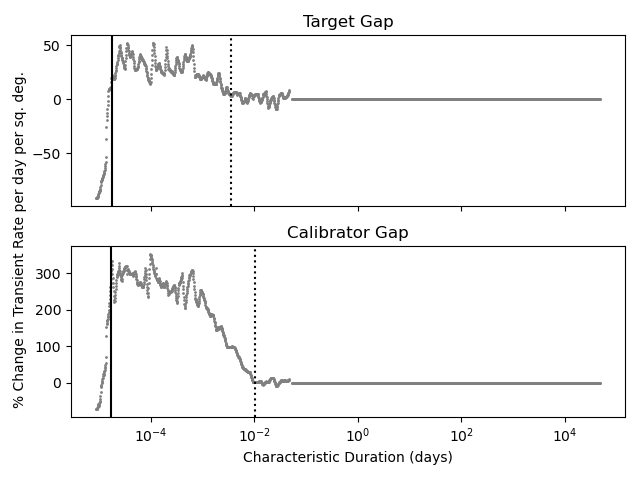
\includegraphics[width=0.75\columnwidth]{figure7.png}
\caption{Percent difference in upper limits on transient rates for transients with a tophat light curve for transients with a peak flux of 0.464 Jy, from no gaps in a survey with 4 hour observations to 5-minute gaps (top) and 15-minute gaps (bottom).}
\label{fig7}
 \end{figure}
 
 \begin{figure}
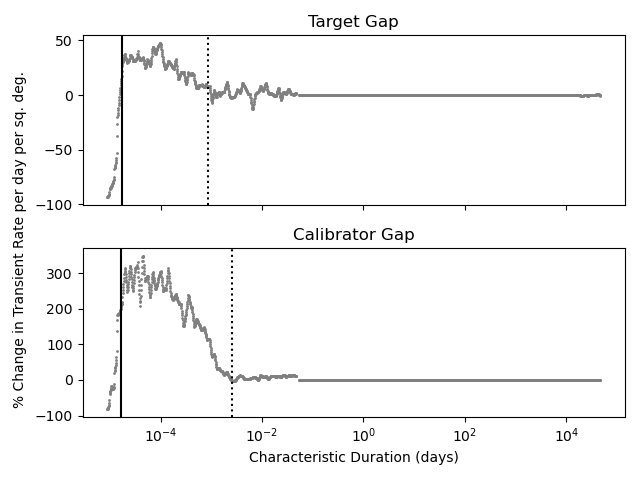
\includegraphics[width=0.75\columnwidth]{figure8.png}
\caption{Percent difference in upper limits on transient rates for transients with a FRED light curve for transients with a peak flux of 0.464 Jy, from no gaps in a survey with 4 hour observations to 5-minute gaps (top) and 15-minute gaps (bottom).}
\label{fig8}
 \end{figure}
 
 \begin{figure}
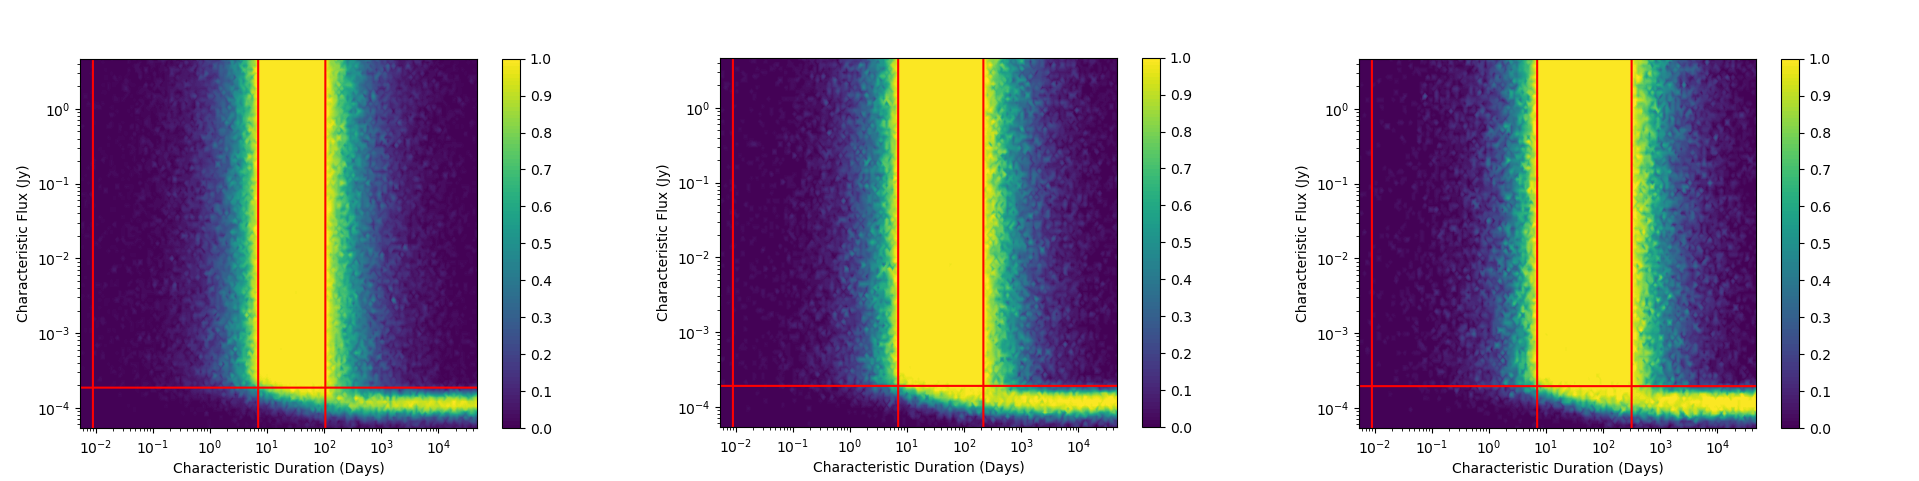
\includegraphics[width=\columnwidth]{threeregion_comboplot.png}
\caption{A probability contour plot for a tophat light curve in a region with no overlap (left), double overlap (center), and triple overlap (right), as seen in Figure~\ref{threepointings}. } 
\label{threeregion}
 \end{figure}

\subsubsection{Multiple Pointings}
Calculating transient rates for multiple overlapping pointings gives a more complete picture of how a survey can probe transient parameter space. An example of such a survey is used here and illustrated in Figure~\ref{threepointings}: three circular fields of view each with a radius of 1.4 degrees. The details are summarized in Tables~\ref{simsurvalt} and~\ref{simsurvseq} below. This setup has seven different regions: three that are probed only by one of the pointings, three that are probed by two pointings, and one that is probed by all three pointings. The three different fields may be observed at various cadences that affect the transient rates in the different areas. If one calculates the probability contours for a tophat transient, as is shown in Figure~\ref{threeregion}, one can compare the single pointing (left) with a double overlapping pointing (middle) and a triple overlapping pointing (right). Note how regions with more overlap have a larger region in the transient duration space where the probability of detecting the transient is equal to 1. 

For a comparison of different survey cadences, one example survey shown in Table~\ref{simsurvalt} alternates between each of the three pointings each week, and another one shown in Table~\ref{simsurvseq} is set up to observe each pointing exclusively before moving to the next one. Figure~\ref{multirgnprob} shows that the probability contours for the triple overlapping region, labelled 0\&1\&2, are the same for both scenarios, as expected. We do, however, see slight differences in the regions with no overlapping pointings in the part of parameter space where transients are best detected. This difference is due to the variations in the maximum gap and survey length in the two survey setups. One particular region with two overlapping pointings, labelled 0\&1, shows the most striking differences between the survey setups. Survey setup 2 produces two of the double overlap regions with good limits on transient rate and one double overlap region with poor limits on the transient rate. In this case, the region that is observed in both the first observed field and the last observed field will have an extremely large gap. Survey setup 1 produces much more consistent detection regions which may suggest that it is the better choice if more uniform transient rate limits are the goal. 

% Relabel survey numbers to make survey one the one on top of the figures 

 \begin{figure}
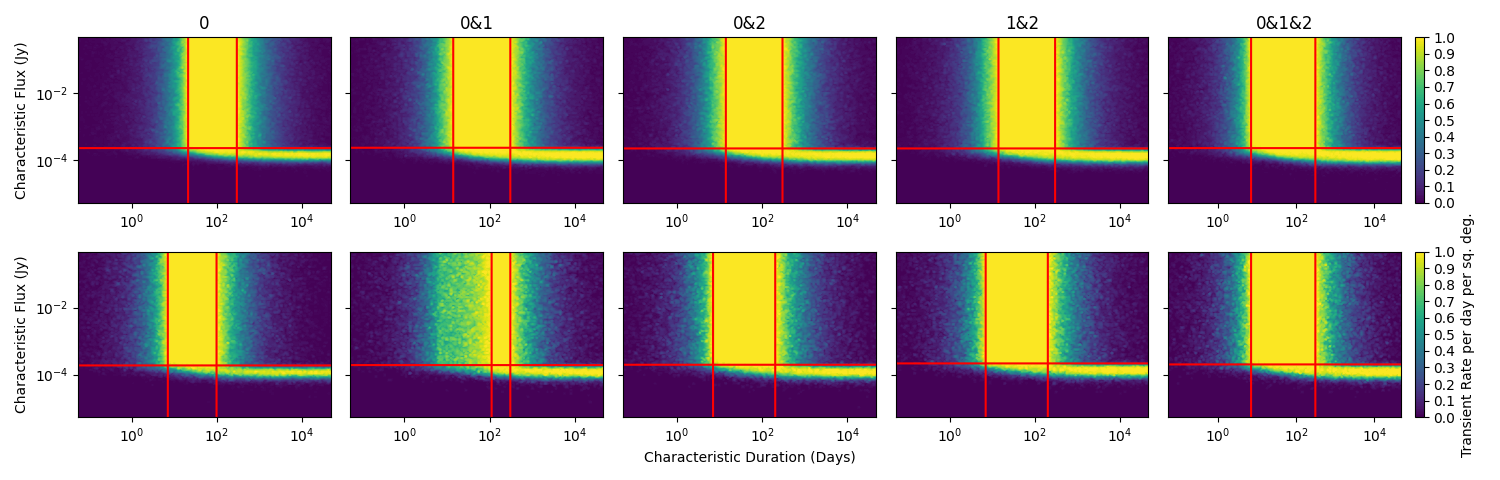
\includegraphics[width=\columnwidth]{multirgnprob.png}
\caption{Probability contours for all of the regions in survey setup 1 (top) and survey setup 2 (bottom). Each pointing is labeled 0, 1 or 2 and the overlap between two pointings are indicated with an `\&', for example 0\&1.}
\label{multirgnprob}
 \end{figure}

\clearpage

\begin{landscape}
\begin{deluxetable}{|c|c|c|c|c|c|c|}
	\tablecolumns{7}
	\tablewidth{0pc}
	\tablecaption{Simulated survey moving between pointings weekly \label{simsurvalt}}
		\tablehead{\colhead{RA (J2000)} & \colhead{DEC }& \colhead{ID }&\colhead{ Area (deg$^2$)} & \colhead{Duration (days)} & \colhead{Start (MJD)} &\colhead{ End}}
		\startdata
		274.7345 & 7.7974 & 0 & 6.1572 & 294.01 & 58997.54 & 58703.53 \\
		275.0913 & 7.1851 & 1 & 6.1572 & 294.01 & 59011.54 & 58717.53 \\
		275.4482& 7.7974 & 2 & 6.1572 & 294.01 & 59004.54 & 58710.53 \\
		274.9130 & 7.4913 & 0\&1 & 4.1987 & 308.01 & 59011.54 & 58703.53 \\
		275.0913 & 7.7975 & 0\&2 & 4.1987 & 301.01 & 59004.54 & 58703.53 \\
		275.2696 & 7.4913 & 1\&2 & 4.1987 & 301.01 & 59011.54 & 58710.53 \\
		275.0913 & 7.5926 & 0\&1\&2 & 3.4360 & 308.01 & 59011.54 & 58703.53 \\
		\enddata
	\end{deluxetable}

\begin{deluxetable}{|c|c|c|c|c|c|c|}
	\tablecolumns{7}
	\tablewidth{0pc}
	\tablecaption{Simulated survey moving between pointings sequentially \label{simsurvseq}}
		\tablehead{\colhead{RA (J2000)} & \colhead{DEC }& \colhead{ID }&\colhead{ Area (deg$^2$)} & \colhead{Duration (days)} & \colhead{Start (MJD)} &\colhead{ End}}
		\startdata
		274.7345 & 7.7974 & 0 & 6.1572 &  98.16 & 58801.70 & 58703.53 \\
		275.0913  & 7.1851 & 1 & 6.1572 &  98.16 & 59011.70 & 58913.53 \\
		275.4482 & 7.7974 & 2 & 6.1572 &  98.16 & 58906.70 & 58808.53 \\
		274.9130 & 7.4913 & 0\&1 & 4.1987 & 308.16 & 59011.70 & 58703.53 \\
		275.0913  & 7.7975 & 0\&2 & 4.1987 & 203.16 & 58906.70 & 58703.53 \\
		275.2696 & 7.4913 & 1\&2 & 4.1987 & 203.16 & 59011.70 & 58808.53 \\
		275.0913  & 7.5926 & 0\&1\&2 & 3.4360 & 308.16 & 59011.70 & 58703.53 \\
		\enddata
	\end{deluxetable}
\end{landscape}
% \geometry{ papersize={8.5in,11in} }

\clearpage
\doublespacing
\subsection{Performance}\label{performance}
Figure~\ref{fig10} shows how the simulations scale in execution time as a function of the number of sources simulated, for the example of 46 observations of 13 minutes with all observations have an identical field-of-view. Figure~\ref{fig11} shows scaling in execution time as a function of the number of observations when the number of sources is held constant at $4.3\times10^{5}$.  All of the simulations for this example were performed on a 2020 Apple Macbook Pro 13 inch model with the M1 chip. In addition to showing the total execution time, key portions of the code are shown as well. The conditionals and flux filtering steps take place when the algorithm is determining if the sources are detected in observations. These steps are so-named because they filter sources based on the calculated integrated flux, and do a large number of boolean and bit operations to calculate and store each transient's state as either detected or not-detected. The stats step is the step that aggregates the detections into probabilities. Finally, the plotting step is where all of the detection statistics, observation information, and false detection information is plotted. Since the data is broken down into a grid in order to plot, the plotting step has no scaling with the number of sources, so it takes a constant amount of time. 

Not shown here are the impacts of a few features and algorithms. The false detection algorithm re-runs the conditionals, flux filtering, and stats steps. In the case of a tophat light curve, this means the false detection algorithm would slightly less than double the amount of time (the plotting step is not doubled). In the case of other light curves, it could have a different impact, usually lower, since the false detection algorithm always uses tophat light curves to simulate constant sources. Another factor not shown here is the impact of having multiple pointings. For example, in a survey setup with two overlapping pointings there will be three regions. Therefore, the run time will be about three times longer than for a single region, assuming equal numbers of observations in each region. 

 \begin{figure}
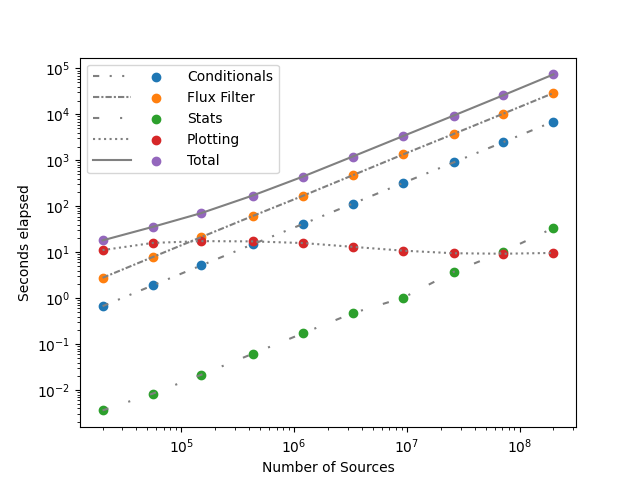
\includegraphics[width=\columnwidth]{figure10.png}
\caption{Execution time as a function of the number of simulated sources.}
\label{fig10}
 \end{figure}
 
  \begin{figure}
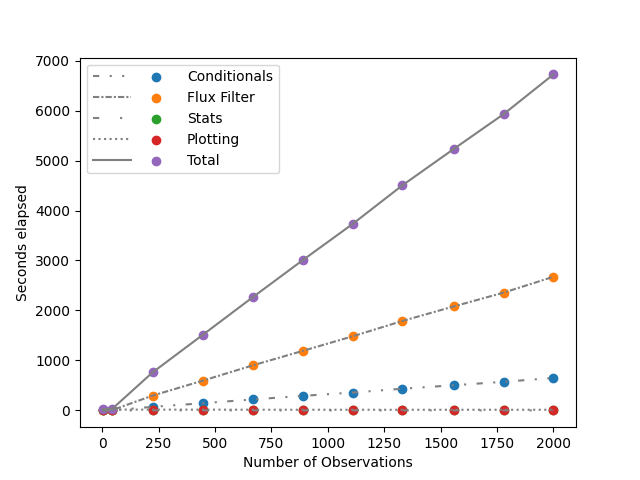
\includegraphics[width=\columnwidth]{figure11.png}
\caption{Execution time as a function of the number of observations.}
\label{fig11}
 \end{figure}
% Make sources vs execution time
% Address impacts of algorithms, 
% Each time per region * regions
% False Det doubles 
% 


\subsection{Future Applications} \label{futureapplications}
\citet{2017MNRAS.465.4106C} shows the existence of a region of 100\% detection probability for the FRED and tophat light curves. The work presented here shows that this region of 100\% detection can be found in a wide variety of light curves. Optimizing the survey parameters to maximize this region of 100\% detection has many potential applications for future surveys. In addition, transient searches can use the false detection calculations to decide the best manner to plan a transient search in a given survey. The wide variety of data outputs can assist with a number of scientific goals that one might have for a survey, and the flexibility of the code can be easily adapted to those purposes.

One application of the code is using the transient simulations to optimize resource allocation. Such optimizations can be done both in terms of survey design and also the data reduction after the observation itself. Simulating a variety of survey setups, such as in section~\ref{Gaps}, is one way to ensure that the survey will accomplish its goals most effectively. In addition, simulations can also be done for varying aspects related to the data reduction, such as the timescale that images are made on. By simulating a combining or splitting up of the observations in a survey into multiple different timescales, one can find an optimal way to search for transients on these multiple time scales with a minimum of re-imaging. These optimizations are becoming increasingly more important with radio facilities such as MeerKAT~\citep{2016mks..confE...1J} and the LOw-Frequency Array (LOFAR)~\citep{2013A&A...556A...2V} which can easily use terabytes of disk space and considerable other computer resources as well. The Square Kilometer Array~\citep{2009IEEEP..97.1482D} and next-generation Very Large Array~\citep{2018ASPC..517....3M}, and other upcoming facilities, will surely require even more resources.

The previously mentioned tools for planning surveys have potential to be expanded to be even more helpful in the future. A potential future update to these simulations could include a tool to help calculate optimal pointings for uniformly probing a large area of the sky in both space and time. 

The simulations code presented in this paper accounts for a large number of realistic effects that complicate transient searches and calculate transient rates from surveys. For research into particular kinds of sources, future upgrades can be made for particular light curves and population numbers that reflect certain sources of interest. 

Finally, even though this simulations code has been designed for surveys in the radio regime, and the examples in this paper are based on this particular use case, it can easily be adapted and applied to other spectral regimes.


\subsection{Conclusions} \label{conclusions}
Simulating transients, following the methodology and code case presented here, allows for calculating transient rates that are highly accurate due to the implementation of a variety of observational effects. The simulations presented here account for a variety of observing sensitivities, pointings, survey cadences, and gaps within observations and surveys. Furthermore, it has been made easy to obtain, since it will be freely available for download through Github, and easy to use through the use of a modular design, the inclusion of scripts to extract metadata from observations, and updates for modern versions of Python.



\subsection{Acknowledgements} 

The authors would like to thank the referee for their constructive comments that helped improve the paper.
The authors would like to acknowledge the ThunderKAT collaboration for the valuable sharing of knowledge and resources, and Michael Moss for his helpful comments and feedback on this manuscript. 
This work was completed in part with resources provided by the High Performance Computing Cluster
at The George Washington University, Information Technology, Research Technology Services.

\subsection{Appendix: Included Light Curves}
%\subsection{Included Light Curves}
\label{sec:lc:appendix}

Here we present and briefly discuss the light curve shapes that are currently included in the simulations code base.

\subsubsection{Tophat}

The tophat is the simplest transient light curve in concept:
\begin{equation}
F=F_{pk}~\text{for}~t_{start} \le t \le t_{end}
\end{equation}
It is simply at the peak flux for the entire duration of the transient. The probability contour plot shown in Figure~\ref{tophat} has a region in parameter space in which all transients are always detected, which can be referred to as a region of guaranteed detection. This region has vertical boundaries that can be found to have a quite straightforward interpretation \citep{2017MNRAS.465.4106C}. The left-most boundary is the longest gap in the observations or, in other words, the longest duration of a tophat transient that could go undetected. The right-most vertical bounding line corresponds to the longest time scale that a transient could have while not being detected as a constant source. This quantity is the duration of the entire survey minus either the first or last observation. 

\subsubsection{Fast Rise Exponential Decay}
The fast rise exponential decay (FRED) light curve is defined as instantaneously rising to the peak flux and exponentially decaying with an characteristic duration $\tau$, defined as its e-folding time:
\begin{equation}
F=F_{pk}\,\exp\left[\frac{-(t-t_{start})}{\tau}\right]~\text{for}~t\ge t_{start}
\end{equation}

This light curve produces a slightly different probability contour, seen in Figure~\ref{fred}, in which the bounding lines for the region of guaranteed detection can be interpreted as follows. The left boundary corresponds to the boundary due to the longest gap, like the tophat. However, unlike the tophat, the flux of the FRED light curve approaches but never actually reaches zero as time progresses. Therefore, brighter transients can be detected for longer than the characteristic duration of the transient, making this boundary a curve instead of a vertical line. The boundary condition can be expressed as $F_{int}=S_{gap}$, i.e. the integrated flux of the transient needs to be equal to the sensitivity of the observation the transient would be detected in, which would be the observation after the gap. We can find the integrated flux:
\begin{equation}
   F_{int} = F_{pk}\,\tau\,\frac{\exp\left[-\frac{\max(T_{start},t_{start})}{\tau}\right] - \exp\left[\frac{T_{end}}{\tau}\right]}{T_{end}-T_{start}} 
\end{equation}
Since we consider the case where the transient starts in the gap, the start of the observation that detects the transient is equal to the length of time from the start of the transient until the end of the gap, which we label $T_{gap}$: $T_{start}=T_{gap}$. 
Therefore, $T_{end}=T_{start}+\Delta T_{gap}$, where $\Delta T_{gap}$ is the duration of the observation. Inserting the integrated flux into the previous equation and solving for $F_{pk}$ yields:
\begin{equation}
F_{pk}(\tau) = \frac{S_{gap}\,\Delta T_{gap}}{\tau\,\left(\exp\left[-\frac{T_{gap}}{\tau}\right] - \exp\left[\frac{(T_{gap} + \Delta T_{gap})}{\tau}\right]\right)}
\end{equation}

The right boundary is the boundary for the longest timescale. We can follow the same procedure as the left boundary, finding that $S_{obs} = S_{last}$, the sensitivity of the last observation in the survey. We also find the following modifications:
\begin{equation}
T_{start} = \tau_{survey}  - \Delta T_{last}
\end{equation}
\begin{equation}
    T_{end} = \tau_{survey}
\end{equation}
\begin{equation}
    F_{pk}(\tau) = \frac{S_{last}\,\Delta T_{last}}{\tau\,\left(\exp\left[-\frac{(\tau_{survey} - \Delta T_{last})}{\tau}\right] - \exp\left[\frac{\tau_{survey}}{\tau}\right]\right)}
\end{equation}


\begin{figure}
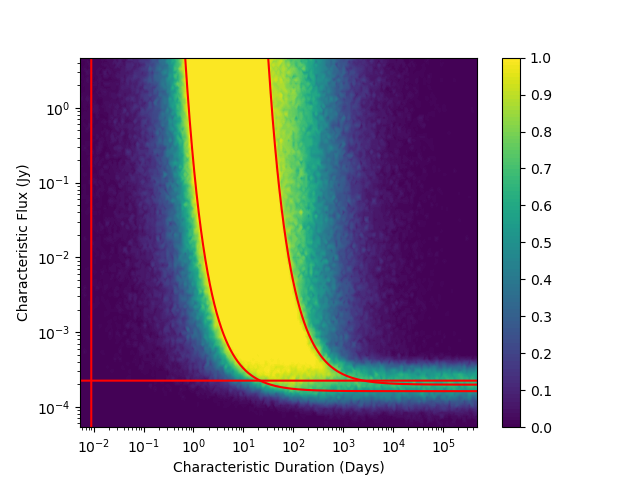
\includegraphics[width=\columnwidth]{wilma.png}
\caption{Probability contours for the Wilma light curve}
\label{wilma}
 \end{figure}
 
\subsubsection{Exponential Rise Fast Decay (Wilma)}
In light of the FRED light curve, a natural extension would be to examine the reverse FRED light curve. The light curve ends at the peak flux and has no definite start:
\begin{equation}F=F_{pk}\,\exp\left[{\frac{(t-t_{end})}{\tau}}\right]\text{ for }t\le t_{end}\end{equation}
The probability contour plot for this light curve is shown in Figure~\ref{wilma}. As one can see, it is identical to the FRED light curve in Figure~\ref{fred}. This makes sense when one realizes that if the entire survey were time-reversed, the light curve would be a FRED. For this reason, the lines bounding the region of guaranteed detection are the same as for the FRED light curve. 

\begin{figure}
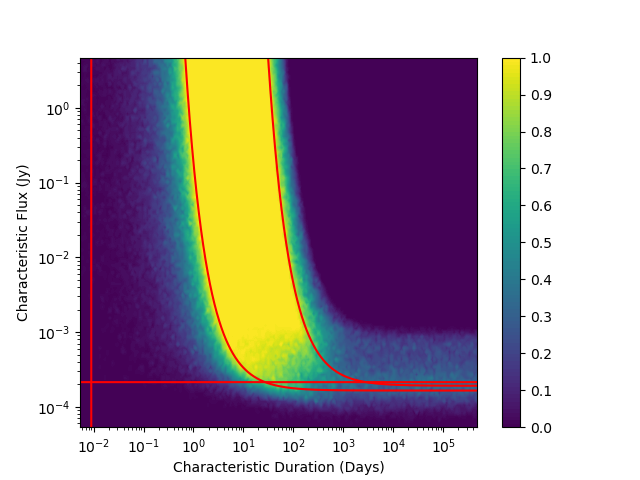
\includegraphics[width=\columnwidth]{ered.png}
\caption{Probability contours for the ERED light curve}
\label{ered}
 \end{figure}
 
\subsubsection{Exponential Rise Exponential Decay}
The Exponential Rise Exponential Decay (ERED) light curve (Figure~\ref{ered}) does not have a definite beginning nor end, only a characteristic time at which the flux is the peak flux and $\tau$, which is its e-folding time:
\begin{equation}F=F_{pk}\,\exp\left[{\frac{(t-t_{char})}{\tau}}\right]\text{ for }t< t_{char}\end{equation}
\begin{equation}F=F_{pk}\text{ for }t=t_{char}\end{equation}
\begin{equation}F=F_{pk}\,\exp\left[{\frac{-(t-t_{char})}{\tau}}\right]\text{ for }t> t_{char}\end{equation}
The transients from this light curve also behave similarly to the previous two cases, since this light curve is a Wilma light curve immediately followed by a FRED light curve.  Therefore, if we use the integrated flux to find the curve marking the boundary corresponding to the shortest duration transient that will always be detected, we find:
\begin{equation}F_{pk}(\tau) = \frac{ S _{gap}\,\Delta T_{gap}}{\frac{\tau}{2}\,\left(\exp\left[-\frac{T_{gap}}{\tau}\right] - \exp\left[\frac{2\Delta T_{gap} + T_{gap}}{\tau}\right]\right)}\end{equation}
Similarly, for the flux limit on the longest timescale, we have:
\begin{equation}F_{pk}(\tau) = \frac{S_{first/last}\,\Delta T_{first/last}}{\frac{\tau}{2}\,\left(\exp\left[-\frac{\tau_{survey}}{\tau}\right] - \exp\left[-\frac{2\Delta T_{first/last} + \tau_{survey}}{\tau}\right]\right)}\end{equation}
In this equation, $S_{first/last}$ and $\Delta T_{first/last}$ would correspond to either the first or last observation in the survey depending on which is more sensitive. 

\subsubsection{Parabola}
Also included is a parabolic light curve defined as follows:
\begin{equation}F = F_{pk}\,\left(1 - \frac{4}{\tau^2}\left(t - \frac{\tau}{2} - t_{crit}\right)^2\right)\end{equation}
$t_{crit}$ is the peak of the light curve, which occurs at half of the duration of the light curve. Since the parabolic light curve starts and ends at zero flux, rather than approaching zero like the exponential or Gaussian light curves, this light curve has a definite duration like the tophat. The light curves with a definite duration all have boundaries in the probability contour plots that are derived in the same way as those for the tophat light curves. The boundaries in the case of the the exponential or Gaussian light curves come about from there being a difference between the characteristic duration and the duration that the transient is actually detected in the observations. 
\subsubsection{Gaussian}
The final light curve included is a Gaussian-shaped one:
\begin{equation}F=F_{pk}\,\exp\left[\frac{-(t-t_{crit})^2}{2\left(\frac{\tau}{2}\right)^2}\right]\end{equation}
In order to find the boundaries for the region of parameter space where the transients are always detected, we follow the same process as we did for the FRED light curve, and find an equation for the integrated flux (with erf being the Gauss error function): 
\begin{equation}
\begin{split}
    F_{int} = F_{pk}\,\tau\,\sqrt{\frac{\pi}{8}}\,(\text{erf}\left[\frac{\sqrt{2}(T_{end}-t_{crit})}{\tau}\right]\\
    -\text{erf}\left[\frac{\sqrt{2}(T_{start}-t_{crit})}{\tau}\right])/(T_{end}-T_{start})
\end{split}
\end{equation}
We can define the boundary on the transient flux needed to be detected as $F_{int}=S_{gap}$.
Using the equation for integrated flux, we find the boundary for the shortest possible duration transient that will always be detected:

\begin{equation}
\begin{split}
    F_{pk} = \frac{S_{obs}\,\Delta T_{obs}}{\tau\, \sqrt{\frac{\pi}{8}}}\frac{1}{\text{erf}\left[\frac{-\Delta T_{gap}}{\sqrt{2}\,\tau}\right] - \text{erf}\left[\frac{(-2\Delta T_{obs} - \Delta T_{gap})}{\sqrt{2}\,\tau}\right]}
\end{split}
\end{equation}

We also find the boundary on the right, for the longest possible duration transient before it is considered a constant source:

\begin{equation}
\begin{split}
    F_{pk} = \frac{S_{obs}\,\Delta T_{obs}}{\tau\, \sqrt{\frac{\pi}{8}}}\frac{1}{\text{erf}\left[\frac{-(\Delta T_{survey} + 2\Delta T_{obs})}{\sqrt{2}\,\tau}\right] - \text{erf}\left[\frac{-\sqrt{2}\,\Delta T_{survey}}{\tau}\right]}
\end{split}
\end{equation}
\newpage
\section{Commensal Transient Searches in 8 Short Gamma-Ray Burst Fields}

Transient searches at radio wavelengths are now yielding an unprecedented number of transients of all kinds. For some time now, transient searches in other wavebands such as the optical and X-rays have yielded a large number of results, and now this is starting to be true for the radio regime as well. Some searches in time series analysis have found transients like fast radio bursts (FRBs) with timescales on the order of milliseconds~\citep[e.g.,][]{2007Sci...318..777L,2021ApJS..257...59C}. Other searches have been performed in radio images, with the number of transients and variables found this way increasing and yielding interesting results. For example, a transient was found in the LOFAR Multi-frequency Snapshot Survey on a timescale of around 10 minutes at 60 MHz~\citep{2016MNRAS.456.2321S}. The CHILES Variable and Explosive Radio Dynamic Evolution Survey~\citep{2021ApJ...923...31S} spent hundreds of hours observing the COSMOS field at 1.4 GHz and found a number of variable sources at timescales from days to years. There have also been transients found as part of a commensal search, that is, a search of data taken as part of a different scientific objective. In commensal transient searches with MeerKAT at 1.3 GHz,~\citet{2020MNRAS.491..560D} find a transient with a timescale of weeks and a variable pulsar on sub-week timescales; and in this same field,~\citet{2022MNRAS.512.5037D} find variable sources on timescales of weeks to months. Similarly,~\citet{2022MNRAS.517.2894R} found four variable sources with timescales spanning from seconds up to over a year. \citet{2022MNRAS.513.3482A} also found a radio transient source in a commensal search of MeerKAT data. As part of the Deeper, Wider, Faster,~\citet{2023MNRAS.519.4684D} have found multiple transients and variables with ASKAP. Additionally, the Variables and Slow Transients survey (VAST) using ASKAP~\citep{2021PASA...38...54M} has found multiple radio transients~\citep{2021ApJ...920...45W,2022MNRAS.516.5972W} and the Very Large Array Sky Survey (VLASS) using the VLA at frequencies around 3 GHz~\citep{2020PASP..132c5001L} promises to find a large number of transients and variables due to their large sky coverage and multi-epoch observing strategies. 

Commensal searches for transients and variables is proving to be a valuable way of probing the radio sky, in particular with facilities that have a large field of view. Not only are commensal searches an efficient use of pre-existing scientific data, they also have the potential to find new and interesting sources as well as increasing our knowledge of the populations of sources on the radio sky by constraining transient rates~\citep[e.g.,][]{2011ApJ...728L..14B,2016MNRAS.459.3161C}. The number of detections along with the survey properties, if used in conjunction with accurate transient rate calculations, can uncover more information about sources with unknown associations. In addition, with calculations that allow for calculating different transient rates for different parts of the sky, such as~\citep{2022ascl.soft04007C}, it is possible to reveal differences in transients and their behavior in different parts of the sky, such as galactic versus extragalactic sources. 

Enabling all of these aforementioned new transient discoveries, with their excellent sensitivity and large field of view, are new facilities such as MeerKAT, ASKAP, and LOFAR~\citep{2009IEEEP..97.1522J,2008ExA....22..151J,2013A&A...556A...2V}. Due to the excellent instantaneous {\it uv} coverage of these instruments, these searches are also able to probe increasingly shorter timescales, with the capability to image on timescales down to seconds, or to create deep images that combine many hours' worth of data. All of these improvements are creating a wealth of new opportunities for commensal transient searches in radio images. 

ThunderKAT~\citep{2016mks..confE..13F} is a large survey project for image plane radio transients with MeerKAT. Taking advantage of the new opportunities provided by MeerKAT is a key part of its mission, as it includes conducting commensal transient searches in MeerKAT imaging data (besides performing follow-up observations of specific transients found in other wavebands). Part of the challenge of these searches are that it requires analyzing a large amount of data, on the order of hundreds of gigabytes to terabytes. In order to search through these images, we use the LOFAR transients pipeline \citep[{\sc TraP};][]{2015A&C....11...25S}, which creates a catalog of sources and their light curves, and tracks the variability of all the sources in the images. Using TraP we conduct a commensal transient search on multiple timescales of short gamma-ray burst observations taken as part of the ThunderKAT project. We establish methodologies and techniques to find new variable sources among the large quantity of sources in this dataset. We also look into whether the variability of these sources is intrinsic or extrinsic (e.g., interstellar scintillation), and draw conclusions to guide future similar studies. 

We will describe the observations and overall data set in the Observations section, and the methodology for the transient search in the Methods section. The results are presented in the Results section and discussed in the Discussion section, with a summary and concluding remarks in the Conclusion.

\subsection{Observations}

We performed a commensal transient search in observations of eight short gamma-ray burst fields originally taken as part of the ThunderKAT project for the purpose of searching for afterglow emission from short gamma-ray bursts. Each observation was about 4 hours in duration including overhead, such as calibrator observations, with the number of observations per field varying. Each 4-hour observation consisted of 15-minute scans with calibrator measurements of a few minutes interspersed. Table~\ref{tab:allobs} lists all the observations that are a part of our transient survey. The observations were calibrated using version 1.1 of the ProcessMeerKAT pipeline~\citep[{\sc ProcessMeerKAT};][]{pminprep}. Observations were taken at L-band, centerted at 1.28 GHz and spanning frequency range from 856 MHz to 1.7 GHz. As part of this calibration process, parts of the spectrum with a large amount of known radio frequency interference (RFI) were flagged including 933 to 960 MHz, 1163 to 1299 MHz, 1524 to 1630 MHz, and 1680 to 1711 MHz. Calibration was performed in parallel by separating the measurement set into 11 spectral windows. The bandpass and complex gain calibration was performed using Common Astronomy Software Applications \citep[{\sc CASA;}][]{2022arXiv221002276T} tools and the calibrators listed in Table~\ref{tab:allobs}. Automated RFI flagging was performed using tfcrop and rflag. After two rounds of calibration and flagging, the spectral windows were recombined into a single measurement set for imaging. 

All images were made using tclean. The 4-hour images were made by producing a shallow image with the cleaning process stopping based on a threshold of 1 mJy; and then self-calibration and flagging for RFI was performed before making the final, deep image stopping at a threshold of around 80 $\mu$Jy. The 15-minute images were made using the self-calibrated measurement set. The imaging parameters used include the multi-term multi-scale imaging algorithm with the w-project gridder. For the 4-hour images, 128 w-planes were used; and for the 15-minute images, 64 w-planes were used. The latter resulted in increased correlated noise in the 15-minute images. 

The shortest imaging timescale of the data is determined by the integration time of the observations, which is 8 seconds for every observation in this survey. On this timescale the imaging parameters were slightly different. The quality of images made using w-projection and those not using w-projection were seen to be quite similar, apart from a slight offset in the spatial coordinates between the two. Therefore, in an effort to save processing time and computational resources, the images were made using the standard gridder without w-projection, using the multi-term multi-scale imaging algorithm that is a part of tclean.


\subsubsection{Image Quality}

The typical noise values roughly follow the expected scaling for noise as a function of observation time $t$, that is $~1/\sqrt(t)$, and are summarized in Table~\ref{tab:noisesummary} below. As the timescales go shorter, the trend is for the variance in the noise values to go larger, with the images on the 8-second timescale showing a large range of values. 31 out of the 47,964 images at the 8-second timescale had a noise that was many orders of magnitude higher than the typical noise distribution, skewing the statistics in a way that is possibly misleading, and therefore we exclude these highest 31 values for noise on this timescale. In the actual analysis we did not perform any additional quality control steps in the version of TraP we used. 


\newgeometry{margin=1.25in} % modify this if you need even more space
\begin{landscape}
\begin{deluxetable}{lllll}	\tablecolumns{5}
	\tablewidth{0pc}
	\tablecaption{All observations used in this study, indicating the observations' start and end times, phase center position, and time spent on the target.
		\label{tab:allobs}}
	\tablehead{\colhead{Name}  &    \colhead{Observation Time }&         \colhead{RA } &        \colhead{DEC} &  \colhead{Time On Target (hrs) } }
	\startdata
	GRB 200219A &  2020-02-21T12:28:44 to 16:28:44 & 342.6385 & -59.1196 &              3.2031  \\
	GRB 200219A &  2020-02-23T12:07:21 to 16:07:21 & 342.6385 & -59.1196 &              3.1986  \\
	GRB 200219A &  2020-02-27T13:52:43 to 17:51:43 & 342.6385 & -59.1196 &              3.1986  \\
	GRB 200411A &  2020-04-12T07:07:12 to 11:09:12 &  47.6641 & -52.3176 &              3.2053  \\
	GRB 200411A &  2020-04-14T11:31:27 to 15:32:27 &  47.6641 & -52.3176 &              3.2031  \\
	Sculptor & 2020-04-16T05:15:42 to 09:17:42 &  11.8875 & -25.2886 &              3.2031  \\ 
	GRB 200411A & 2020-04-18T07:27:35 to 11:29:35 &  47.6641 & -52.3176 &              3.2009 \\
	GRB 200522A & 2020-05-23T06:56:37 to 11:10:37 &   5.6820 &  -0.2832 &              3.4496 \\
	GRB 200522A & 2020-05-24T06:01:09 to 10:15:09 &   5.6820 &  -0.2832 &              3.4496 \\
	GRB 200522A & 2020-05-29T02:11:13 to 06:24:13 &   5.6820 &  -0.2832 &              3.4452 \\
	GRB 200522A & 2020-06-06T02:01:14 to 06:15:44 &   5.6820 &  -0.2832 &              3.4474 \\
	GRB 200907B & 2020-09-08T01:03:47 to 05:23:17 &  89.0290 &   6.9062 &              3.4430 \\
	GRB 200907B & 2020-09-10T01:47:12 to 06:05:42 &  89.0290 &   6.9062 &              3.4541 \\
	GRB 200907B & 2020-09-14T01:35:52 to 05:54:16 &  89.0290 &   6.9062 &              3.4585 \\
	GRB 200907B & 2020-09-25T02:17:12 to 06:34:54 &  89.0290 &   6.9062 &              3.4563 \\
	GRB 210323A & 2021-03-25T06:17:56 to 10:37:26 & 317.9461 &  25.3699 &              3.4519 \\
	GRB 210323A & 2021-03-27T06:03:55 to 10:23:16 & 317.9461 &  25.3699 &              3.4519 \\
	GRB 210323A & 2021-04-01T05:37:48 to 09:57:17 & 317.9461 &  25.3699 &              3.4563 \\
	GRB 210726A & 2021-07-28T14:24:49 to 17:50:28 & 193.2909 &  19.1875 &              2.7122 \\
	GRB 210726A & 2021-08-01T12:28:16 to 16:47:14 & 193.2909 &  19.1875 &              3.4519 \\
	GRB 210726A & 2021-08-07T12:07:14 to 16:26:20 & 193.2909 &  19.1875 &              3.4519 \\
	GRB 210726A & 2021-08-19T12:18:07 to 16:36:33 & 193.2909 &  19.1875 &              3.4519 \\
	GRB 210726A & 2021-09-06T11:38:11 to 15:56:29 & 193.2909 &  19.1875 &              3.4496 \\
	GRB 210919A & 2021-09-20T01:22:10 to 05:40:20 &  80.2545 &   1.3115 &              3.4519 \\
	GRB 210919A & 2021-09-24T02:49:58 to 07:08:40 &  80.2545 &   1.3115 &              3.4541 \\
	GRB 210726A & 2021-09-26T09:35:20 to 13:54:18 & 193.2909 &  19.1875 &              3.4563 \\
	GRB 210919A & 2021-09-27T01:23:09 to 05:41:27 &  80.2545 &   1.3115 &              3.4541 \\
	GRB 210323A & 2021-09-30T17:35:55 to 21:56:06 & 317.9461 &  25.3699 &              3.4541 \\
	GRB 210726A & 2021-12-27T02:48:11 to 07:07:17 & 193.2909 &  19.1875 &              3.4430 \\
	GRB 210726A & 2021-09-26T09:35:20 to 13:54:18 & 193.2909 &  19.1875 &              3.4563  \\
	GRB 210919A & 2021-09-27T01:23:09 to 05:41:27 &  80.2545 &   1.3115 &              3.4541\\
	GRB 210323A & 2021-09-30T17:35:55 to 21:56:06 & 317.9461 &  25.3699 &              3.4541 \\
	GRB 210726A & 2021-12-27T02:48:11 to 07:07:17 & 193.2909 &  19.1875 &              3.4430 \\
	\enddata
\end{deluxetable}
\end{landscape}
\begin{deluxetable}{lll}	\tablecolumns{3}
	\tablewidth{0pc}
	\tablecaption{Calibrators used for each field in this study.
		\label{tab:allobscals}}
	\tablehead{\colhead{Name}  & \colhead{Bandpass Calibrator} & \colhead{Gain Calibrator}}
	\startdata
	GRB 200219A & J0408-6545 & J2329-4730 \\
	GRB 200411A & J0408-6545 & J0210-5101 \\
	Sculptor & J1939-6342 & J0025-2602 \\
	GRB 200411A  & J0408-6545 & J0210-5101 \\
	GRB 200522A  & J1939-6342 & J0022+0014 \\
	GRB 200907B  & J0408-6545 & J0521+1638 \\
	GRB 210323A  & J1939-6342 & J2236+2828 \\
	GRB 210726A  & J1331+3030 & J1330+2509 \\
	GRB 210919A  & J0408-6545 & J0503+0203 \\
	\enddata
\end{deluxetable}

\clearpage
\restoregeometry
 \doublespacing
\begin{deluxetable}{llll}
	\tablecolumns{4}
	\tablewidth{0pc}
	\tablecaption{Summary of the mean, median and range of the image noise distributions at each timescale in our study. 
		Note that the 8-second timescale statistics are computed with the highest 31 noise values excluded.
		\label{tab:noisesummary}}
		\tablehead{\colhead{Timescale} & \colhead{Range ($\mu$Jy)} & \colhead{Median ($\mu$Jy)} & \colhead{Mean ($\mu$Jy)}}
		\startdata
		4 hours & 6 to 32 & 10 & 13 \\
		15 minutes & 19 to 184 & 30 & 43 \\
		8 seconds & 106 to 17709 & 176 & 205 \\ 
		\enddata
	\end{deluxetable}


\begin{deluxetable}{l|c|c|c}
	\tablecolumns{4}
	\tablewidth{0pc}
	\tablecaption{Summary of number of images of each field at each timescale. \label{tab:obstimescales}}
\tablehead{\colhead{Target} & \colhead{4 hour images} & \colhead{15 minute images} & \colhead{8 second images}}
\startdata
GRB200219A &	4&	51&	5552\\
GRB200411A &	3&	39&	4365\\
Sculptor	&1	&13&	1455\\
GRB200522A	&4&	54&	6265\\
GRB200907B&	4&	56&	6274\\
GRB210323A&	4&	56&	6275\\
GRB210726A&	7&	95&	9072\\
GRB210919A&	3&	42&	4706\\
\enddata
\end{deluxetable}




\subsection{Methods}

\subsubsection{Transient Searches with the LOFAR Transients Pipeline}

After calibrating the data and producing images, the latter were run through the TraP~\citep{2015A&C....11...25S} version 4. While originally designed for LOFAR, the TraP is telescope-agnostic and well suited for any kind of image based radio transient search. When running the images through the pipeline, a detection threshold of 5$\sigma$ was used, which is the threshold for blind detection of a source, along with an analysis threshold of $3\sigma$, which is the threshold used for analyzing information about the source (such as position and flux, and uncertainties in those quantities). The detection threshold was set to 5$\sigma$ instead of the default 8$\sigma$ so that more sources would be detected and analyzed by TraP. We later increase this threshold and reduce the number of candidate transients and variables through additional analysis, as described in section ``Determining Candidate Variables and Transients.'' This process of starting with a lower threshold and increasing it later was beneficial for capturing longer portions of variable light curves since, when a variable source reaches the detection threshold in TraP, the TraP does not go back to previous images to measure the flux of the source before detection. The TraP calculates variability statistics $V$ and $\eta$, which the user can use to classify a source as constant or varying. These statistics are as defined in \citet{2015A&C....11...25S}:
\begin{equation}\label{Veqn}
    V_{\nu} = \frac{1}{\bar{I}_{\nu}}\sqrt{\frac{N}{N-1} (\bar{I_{\nu}^2} - \bar{I_{nu}}^2)}
\end{equation}
\begin{equation}\label{etaeqn}
    \eta =  \frac{1}{N-1} \sum_{i=1}^{N} \frac{(I_{\nu,i} - \xi_{I_{\nu}})^2}{\sigma_{\nu,i}^2}   
\end{equation}
In these equations, $\nu$ is the observing frequency, $I$ is the flux measurement, $N$ is the number of observations, $\xi$ is the weighted mean flux density (whose weights are the $1/\sigma_{\nu}^2$), $\sigma$ is the uncertainty in flux measurement, and the bar over a quantity indicates an average. 

The transient search on the 8-second timescale was limited in time to the images contained within an approximately 15 minute scan in order to improve variability statistics and due to the warping of the coordinates in the images. Furthermore, the beamwidths limit in the TraP parameters was set to 3, which relaxes the hard limits on the association between sources that are spatially separated. After searching each of these 15 minutes for transients, the images containing transients were then re-imaged using w-projection, and then compared with the previous images to acquire a corrected position. The number of images for each field is shown in Table~\ref{tab:obstimescales}. Initial runs used 10 deblending thresholds, which is intended to separate sources that are very close together into separate sources; however, due to errors involving source identification and the database within TraP in which an extremely large number of sources were located at the same coordinates in the images, later runs used zero deblending thresholds. This change does not affect any potential transient or variable sources, since these sources would have been clustered close together and discarded in the next step when we restrict the number of sources within 5 times the major axis of the beam (see below).

The output from TraP contains a large number of sources, many of which are not astrophysical but features resulting from imaging artifacts such as sidelobes. These imaging artifacts tend to show up as patterns of bright and dark spots around a relatively bright source. In order to eliminate these sources, sources within a region of a radius of 5 times the major axis of the point-spread function of the brightest sources are discarded. The radius, in beamwidths, was determined through some trial-and-error, and in future studies can be increased to reduce artifacts detected as transients or decreased to reduce the chance of eliminating sources that happen to be tightly clustered in the image. The deep 4-hour images were also examined for each field, and regions excluded from the transient search were created around areas of poor quality due to extremely bright sources. 


\subsubsection{Determining Candidate Variables and Transients}
\label{sec:determinecand}
One challenge of performing transient searches is deciding on the appropriate signal-to-noise cut for a source detection. For this study we adopt the methodology used in~\citet{2022MNRAS.517.2894R}: we fit the flux values of all the pixels in the images to a Gaussian, to determine the sigma threshold that would result in less than one false positive. In the case of the 15-minute and 8-second images, we use a sub-set of the images as a sample, 50\% and 2.5\% of the images, respectively. These sample sizes were constrained by the size of memory of the machine used to compute the threshold. In order to scale up the calculated thresholds to account for the images that were not selected, we used a scaling factor to scale up to the number of pixels that would be in the entire dataset. We then used the quantile function of the Gaussian distribution to determine the sigma threshold that would result in less than one false positive. We did this for all fields combined together but for every timescale separately, and found that the thresholds are approximately 5.3$\sigma$, 5.7$\sigma$, and 6.4$\sigma$ for the 4-hour, 15-minute, and 8-second images respectively. We then reduced the number of potentially interesting sources to investigate by making cuts based on these sigma thresholds, excluded regions, and proximity to neighboring sources.
\begin{figure}
	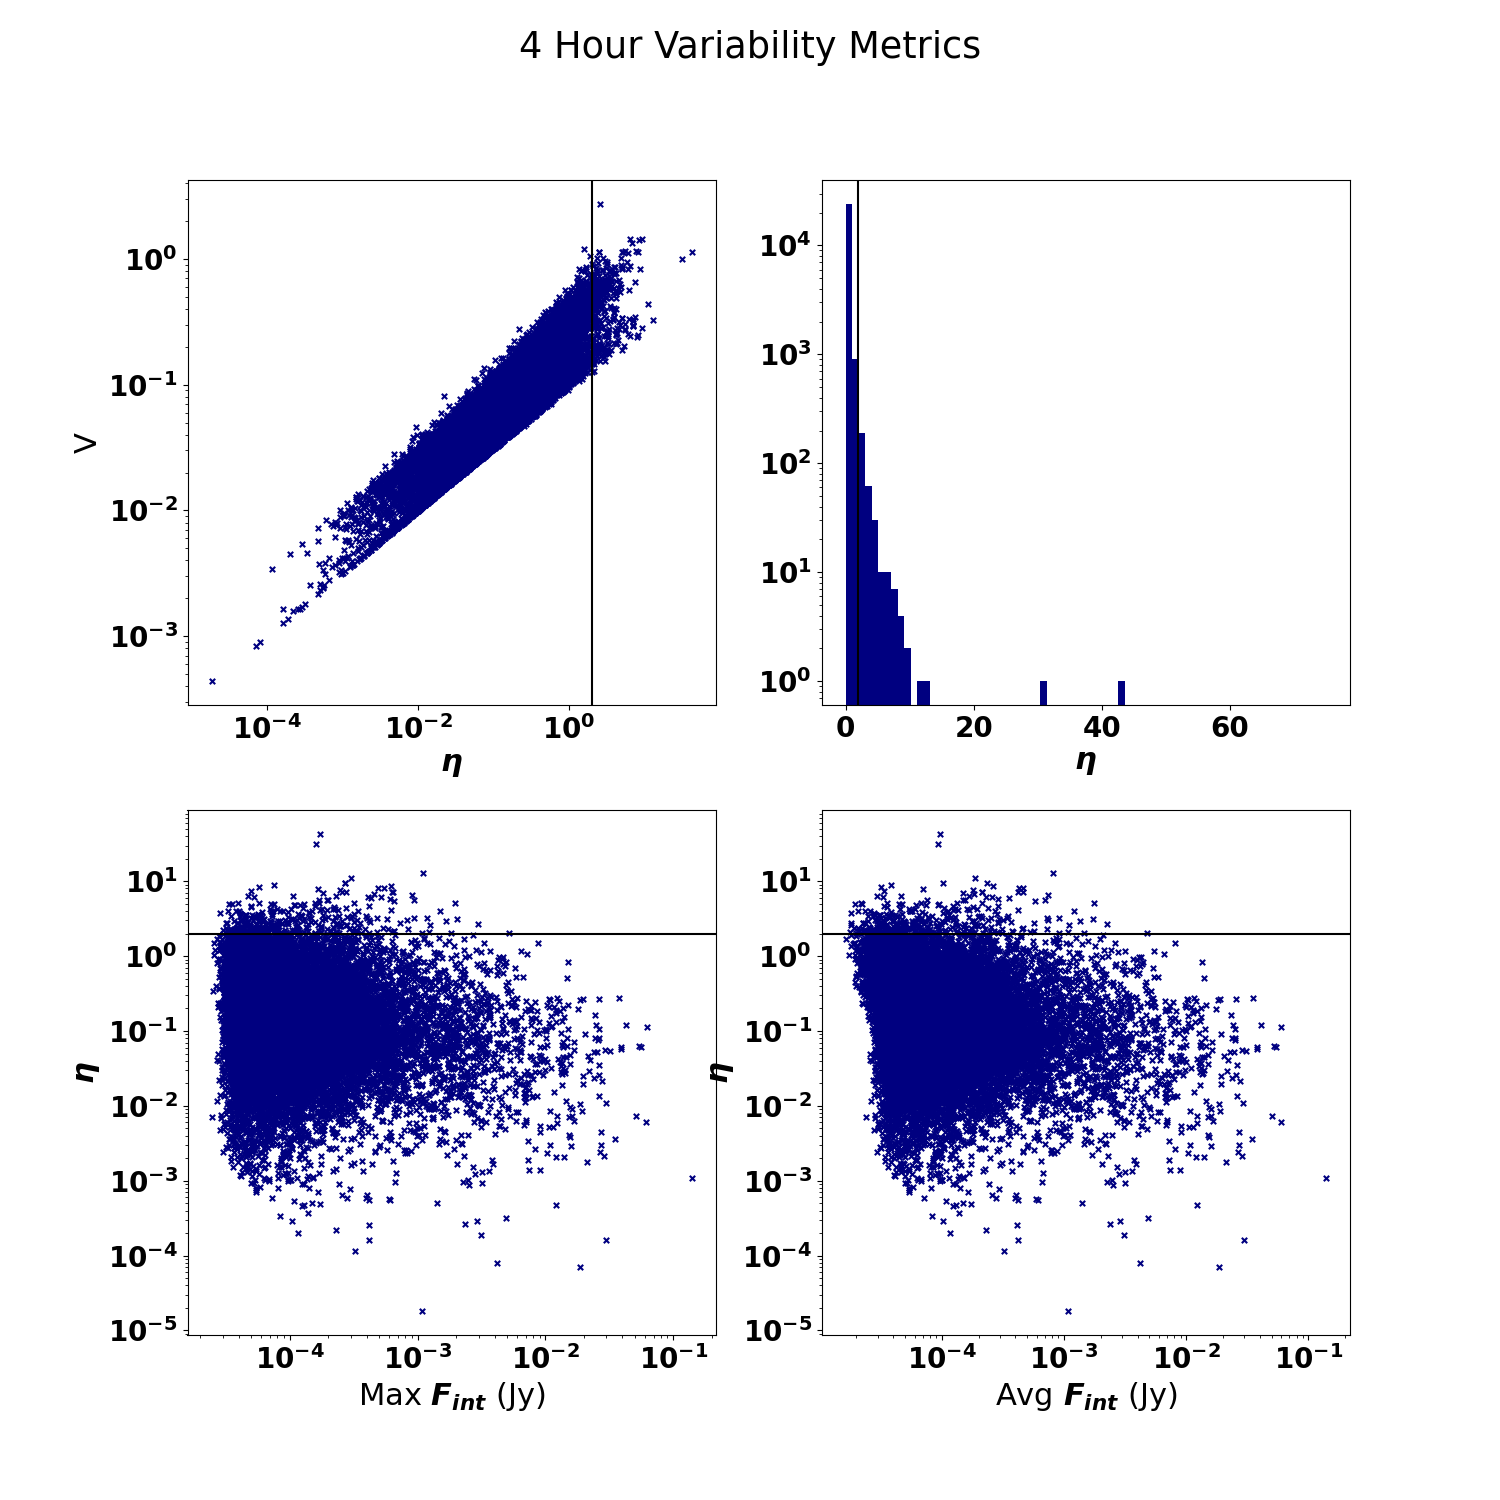
\includegraphics[width=0.9\textwidth]{4_Hour_Variability_Metrics.png}
	\caption{Variability statistics $V$ and $\eta$, as defined in equations~\ref{Veqn} and~\ref{etaeqn}, for the 4-hour timescale, also versus the maximum and average integrated flux. A black vertical line marks $\eta=2$.}
	\label{fig:varstat4hr}
\end{figure}

\begin{figure}
	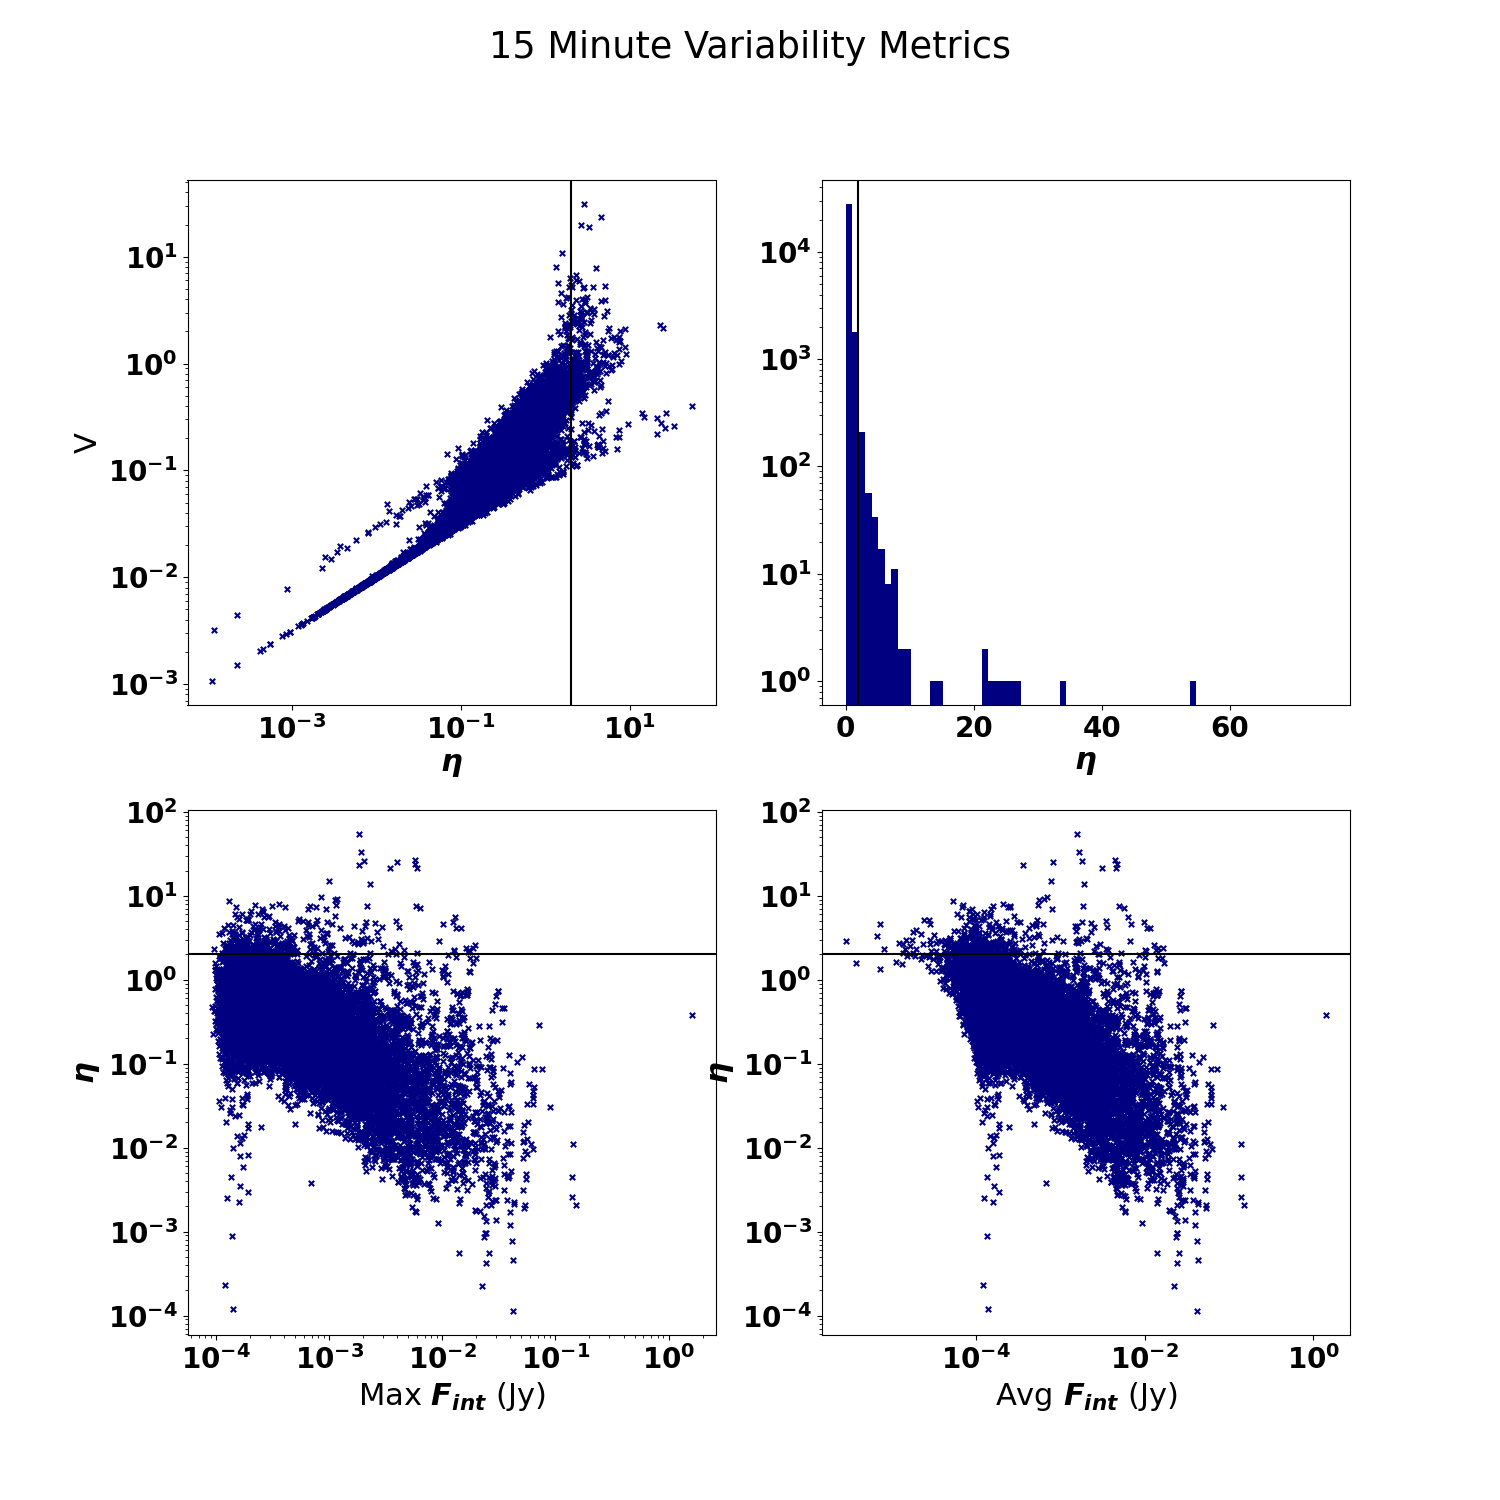
\includegraphics[width=0.9\textwidth]{15_Minute_Variability_Metrics.png}
	\caption{Variability statistics $V$ and $\eta$, as defined in equations~\ref{Veqn} and~\ref{etaeqn}, for the 15-minute timescale, also versus the maximum and average integrated flux. A black vertical line marks $\eta=2$.}
	\label{fig:varstat15min}
\end{figure}

\begin{figure}
	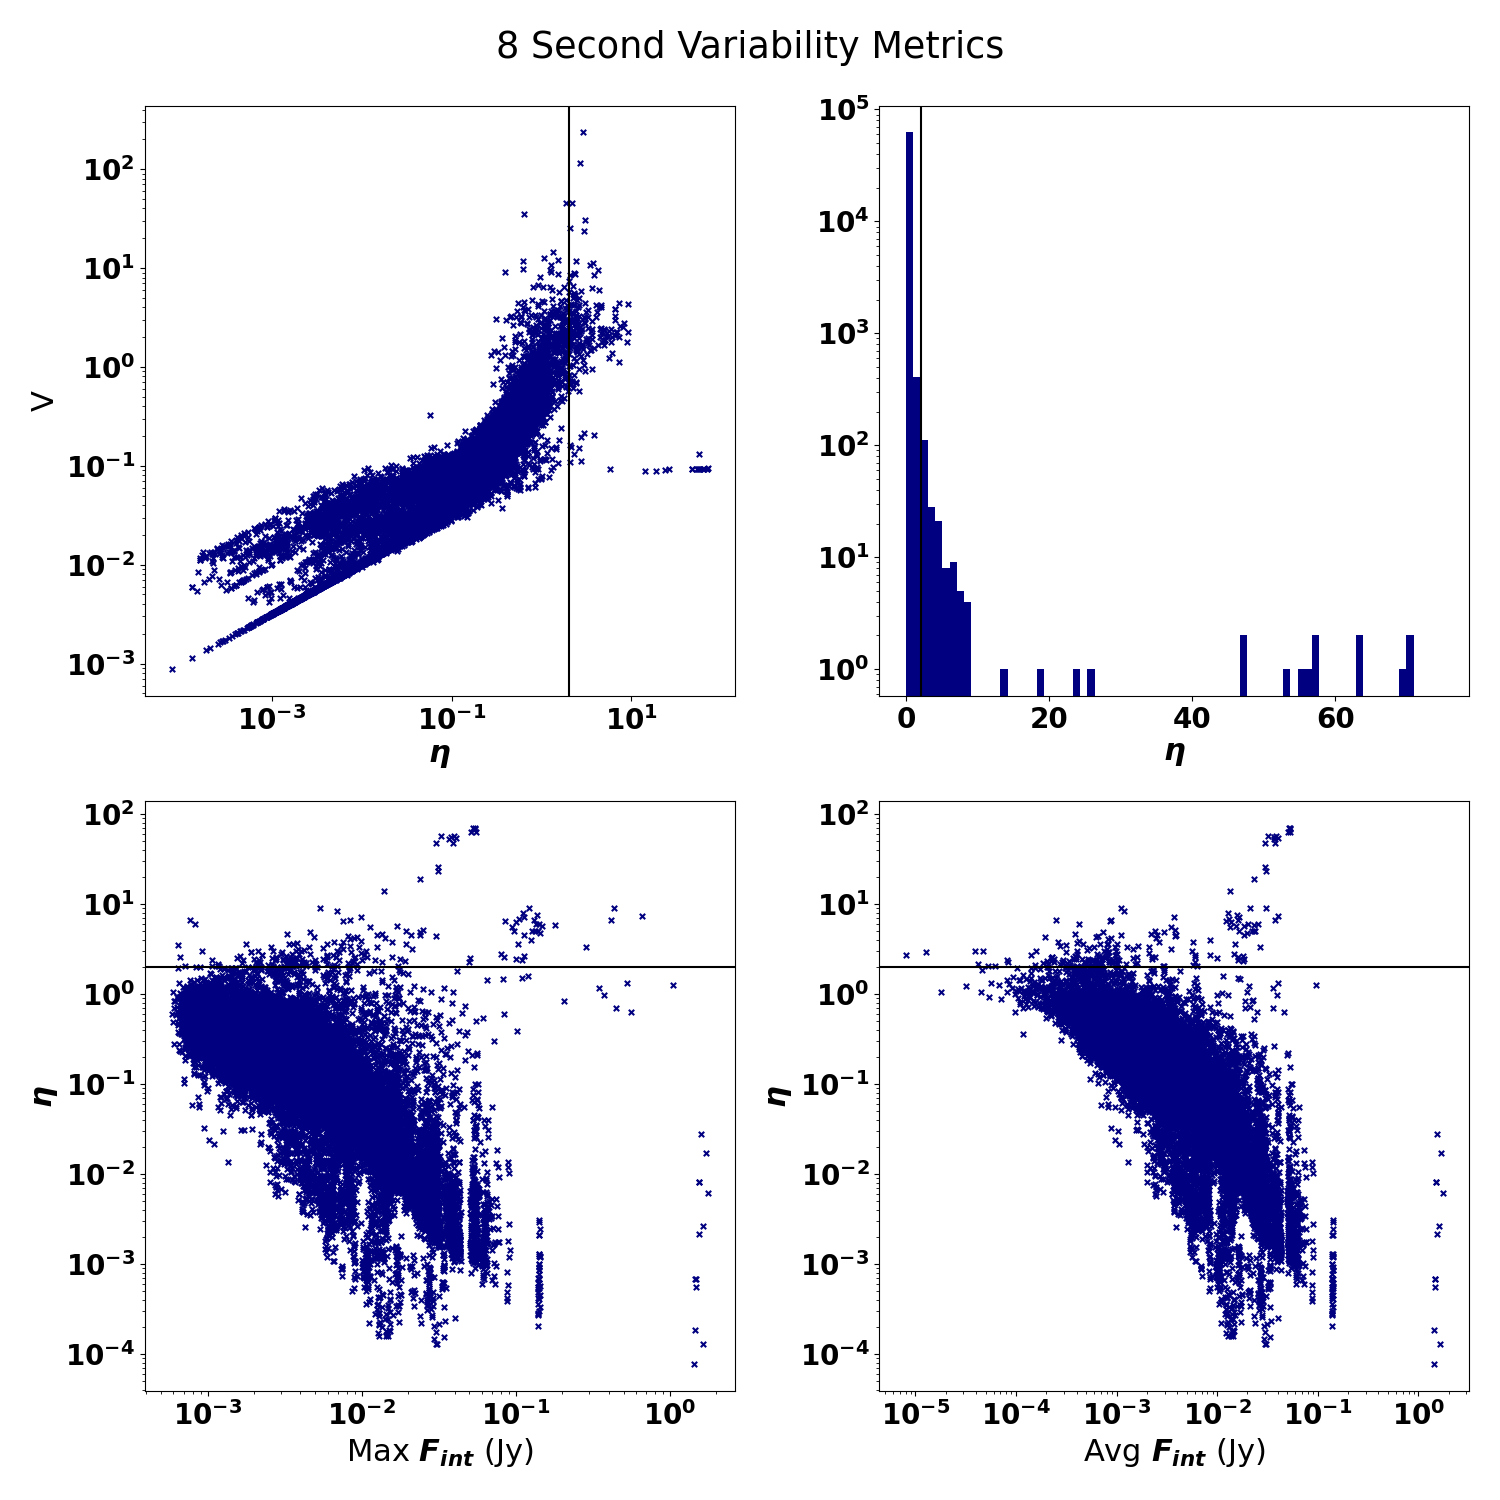
\includegraphics[width=0.9\textwidth]{8_Second_Variability_Metrics.png}
	\caption{Variability statistics $V$ and $\eta$, as defined in equations~\ref{Veqn} and~\ref{etaeqn}, for the 8-second timescale, also versus the maximum and average integrated flux. A black vertical line marks $\eta=2$.}
	\label{fig:varstat8sec}
\end{figure}

After removing potential transients that fall below the signal-to-noise thresholds determined above, in order to determine which sources are potentially variable or transient, we recalculate the variability statistic $\eta$ accounting for a $10\%$ systematic error in flux in the uncertainty, $\sigma$, shown in equation~\ref{etaeqn}, since the value that the TraP calculates for $\eta$ does not include systematic errors that can arise due to instrumental effects and/or calibration errors. We then create animations to examine all sources with a corrected $\eta$ above a value of 2. This value was chosen for practicality reasons, since it represents a value of $\eta$ that indicates significant variability and results in a number of sources that could be practically examined in a non-automated way. This resulted in 214 sources in the 8-second images, 306 sources in the 15-minute images, and 278 sources in the 4-hour images. The images of the sources over time were turned into the aforementioned animations with light curves and variability parameters plotted\footnote{Code available at https://github.com/dentalfloss1/sharedscripts as FindOutliers.py}. Using these animations along with light curves, the sources were sorted by eye into one of the following categories: potentially interesting astrophysical transients, obvious noise artifacts, misassociation errors, and moving objects. The moving objects were only found on the 8-second timescale and are most likely due to RFI, due to the narrow-band behavior of the few sources bright enough for spectral analysis. The objects classified as noise artifacts were mostly from large noise patterns across the field that were mistakenly detected as sources. The misassociation issues came from a number of sources, but most of them due to sidelobes around bright sources. 


\subsection{Results}
\label{sec:results2}
After examining the sources by eye, the number of potential astrophysical transients was three in the 8-second images, 19 in the 15-minute images, and 227 in the 4-hour images. To examine the potential transients on the 8-second timescale, corrected positions were acquired by making w-projected images of all of the 8-second integrations that made up the two scans closest to the time in which the transient appears. Then, a second run through the TraP was done with a forced fit at the corrected position of the transient location. After this process, due to changes in the noise from w-projection, all three potential transients fell below the detection threshold of 6.4$\sigma$ that we previously determined. We followed a similar process for the 15 minute images, forcing a fit at the location of the transients on the 15-minute timescale. After this process, we recalculated the corrected $\eta$ for these sources and no candidates remained at this timescale. Plots showing the flux and variability statistics of the sources on the three different timescales are shown in Figures~\ref{fig:varstat4hr}-\ref{fig:varstat8sec}.

All of the candidates in the 4 hour images were variables. To ensure that these variations were significant, we used the katbeam library to correct for the sensitivity of the primary beam~\citep{2022AJ....163..135D}. We then once again did a forced fit at all of the sources' locations. As a result of the force fitting and once again recalculating a corrected $\eta$, we find 122 sources that still have a corrected $\eta$ greater than two. These sources are all considered to be candidate variables. 
% Numbers subject to change 
\subsubsection{Matching Catalogs}
\label{sec:MatchingCatalogs}
In order to better understand the variable sources, a search was performed of catalogs available within Vizier~\citep[]{vizier} using the Astroquery python library~\citep{2019AJ....157...98G}. These catalogs include other radio catalogs such as FIRST, VLASS,  and NVSS \citep{2015ApJ...801...26H,2021ApJS..255...30G,1998AJ....115.1693C}, in addition to a large number of optical, infrared, and near-infrared catalogs, and some X-ray and gamma-ray catalogs. Notably some of the fields in this survey lack significant multi-wavelength observations due to a lack of surveys from observatories in the southern hemisphere. In addition to searching Vizier, we also searched the Living Swift XPS catalog~\citep{2022MNRAS.tmp.2790E} for X-ray counterparts. The closest LSXPS source to any of our variable sources was approximately 65 arcseconds away, and therefore we conclude that there are no matches in this catalog. For the other catalogs, of the 122 variables in the 4-hour images, 99 of them have a source in other catalogs that are within one arcsecond, which we consider a catalog match. There are 23 sources with no catalog matches, which are given in Table~\ref{tab:unmatched}. 17 of these sources are at southern declinations where there is a lack of catalog data. However, five of these sources should be visible to many different facilities. The lack of a catalog match to these sources could be due to properties of the source, such as the spectral index or intervening material, and the lack of matches in radio catalogs could be due to their relatively low observed flux level on the order of hundreds of $\mu$Jy.



\begin{deluxetable}{lll}
	\tablecolumns{3}
	\tablewidth{0pc}
	\tablecaption{23 variable sources with no multi-wavelength counterparts and their positions in the MeerKAT images. \label{tab:unmatched}}
	\tablehead{\colhead{id} & \colhead{RA} & \colhead{Dec} \\
      & \colhead{(deg)} & \colhead{(deg)}}
	\startdata
	693964 &  344.1593 & -59.5321 \\
	694324 &  343.5354 & -58.8087   \\
	694542 &  343.3390 & -58.9357 \\
	695276 &  342.8254 & -58.5346 \\
	696983 &  341.6460 & -59.6791 \\
	713623 &   89.7308 &   6.6844   \\
	713985 &   89.5435 &   6.3984   \\
	714170 &   89.4624 &   6.9762   \\
	714807 &   89.2317 &   7.0995 \\
	716711 &   88.4060 &   6.6692   \\
	702092 &   48.5602 & -52.5190 \\
	702209 &   48.4860 & -52.0438 \\
	702355 &   48.4381 & -52.7810 \\
	702639 &   48.3066 & -52.7748   \\
	702999 &   48.1607 & -52.0628 \\
	705197 &   47.4973 & -52.3007 \\
	705414 &   47.4271 & -51.9934 \\
	707028 &   46.8995 & -51.7947 \\
	707094 &   46.8666 & -51.7357 \\
	708405 &   48.1628 & -51.5325 \\
	708781 &   47.5189 & -51.6759 \\
	709415 &   46.3704 & -52.3510 \\
	\enddata
\end{deluxetable}

\begin{figure}
	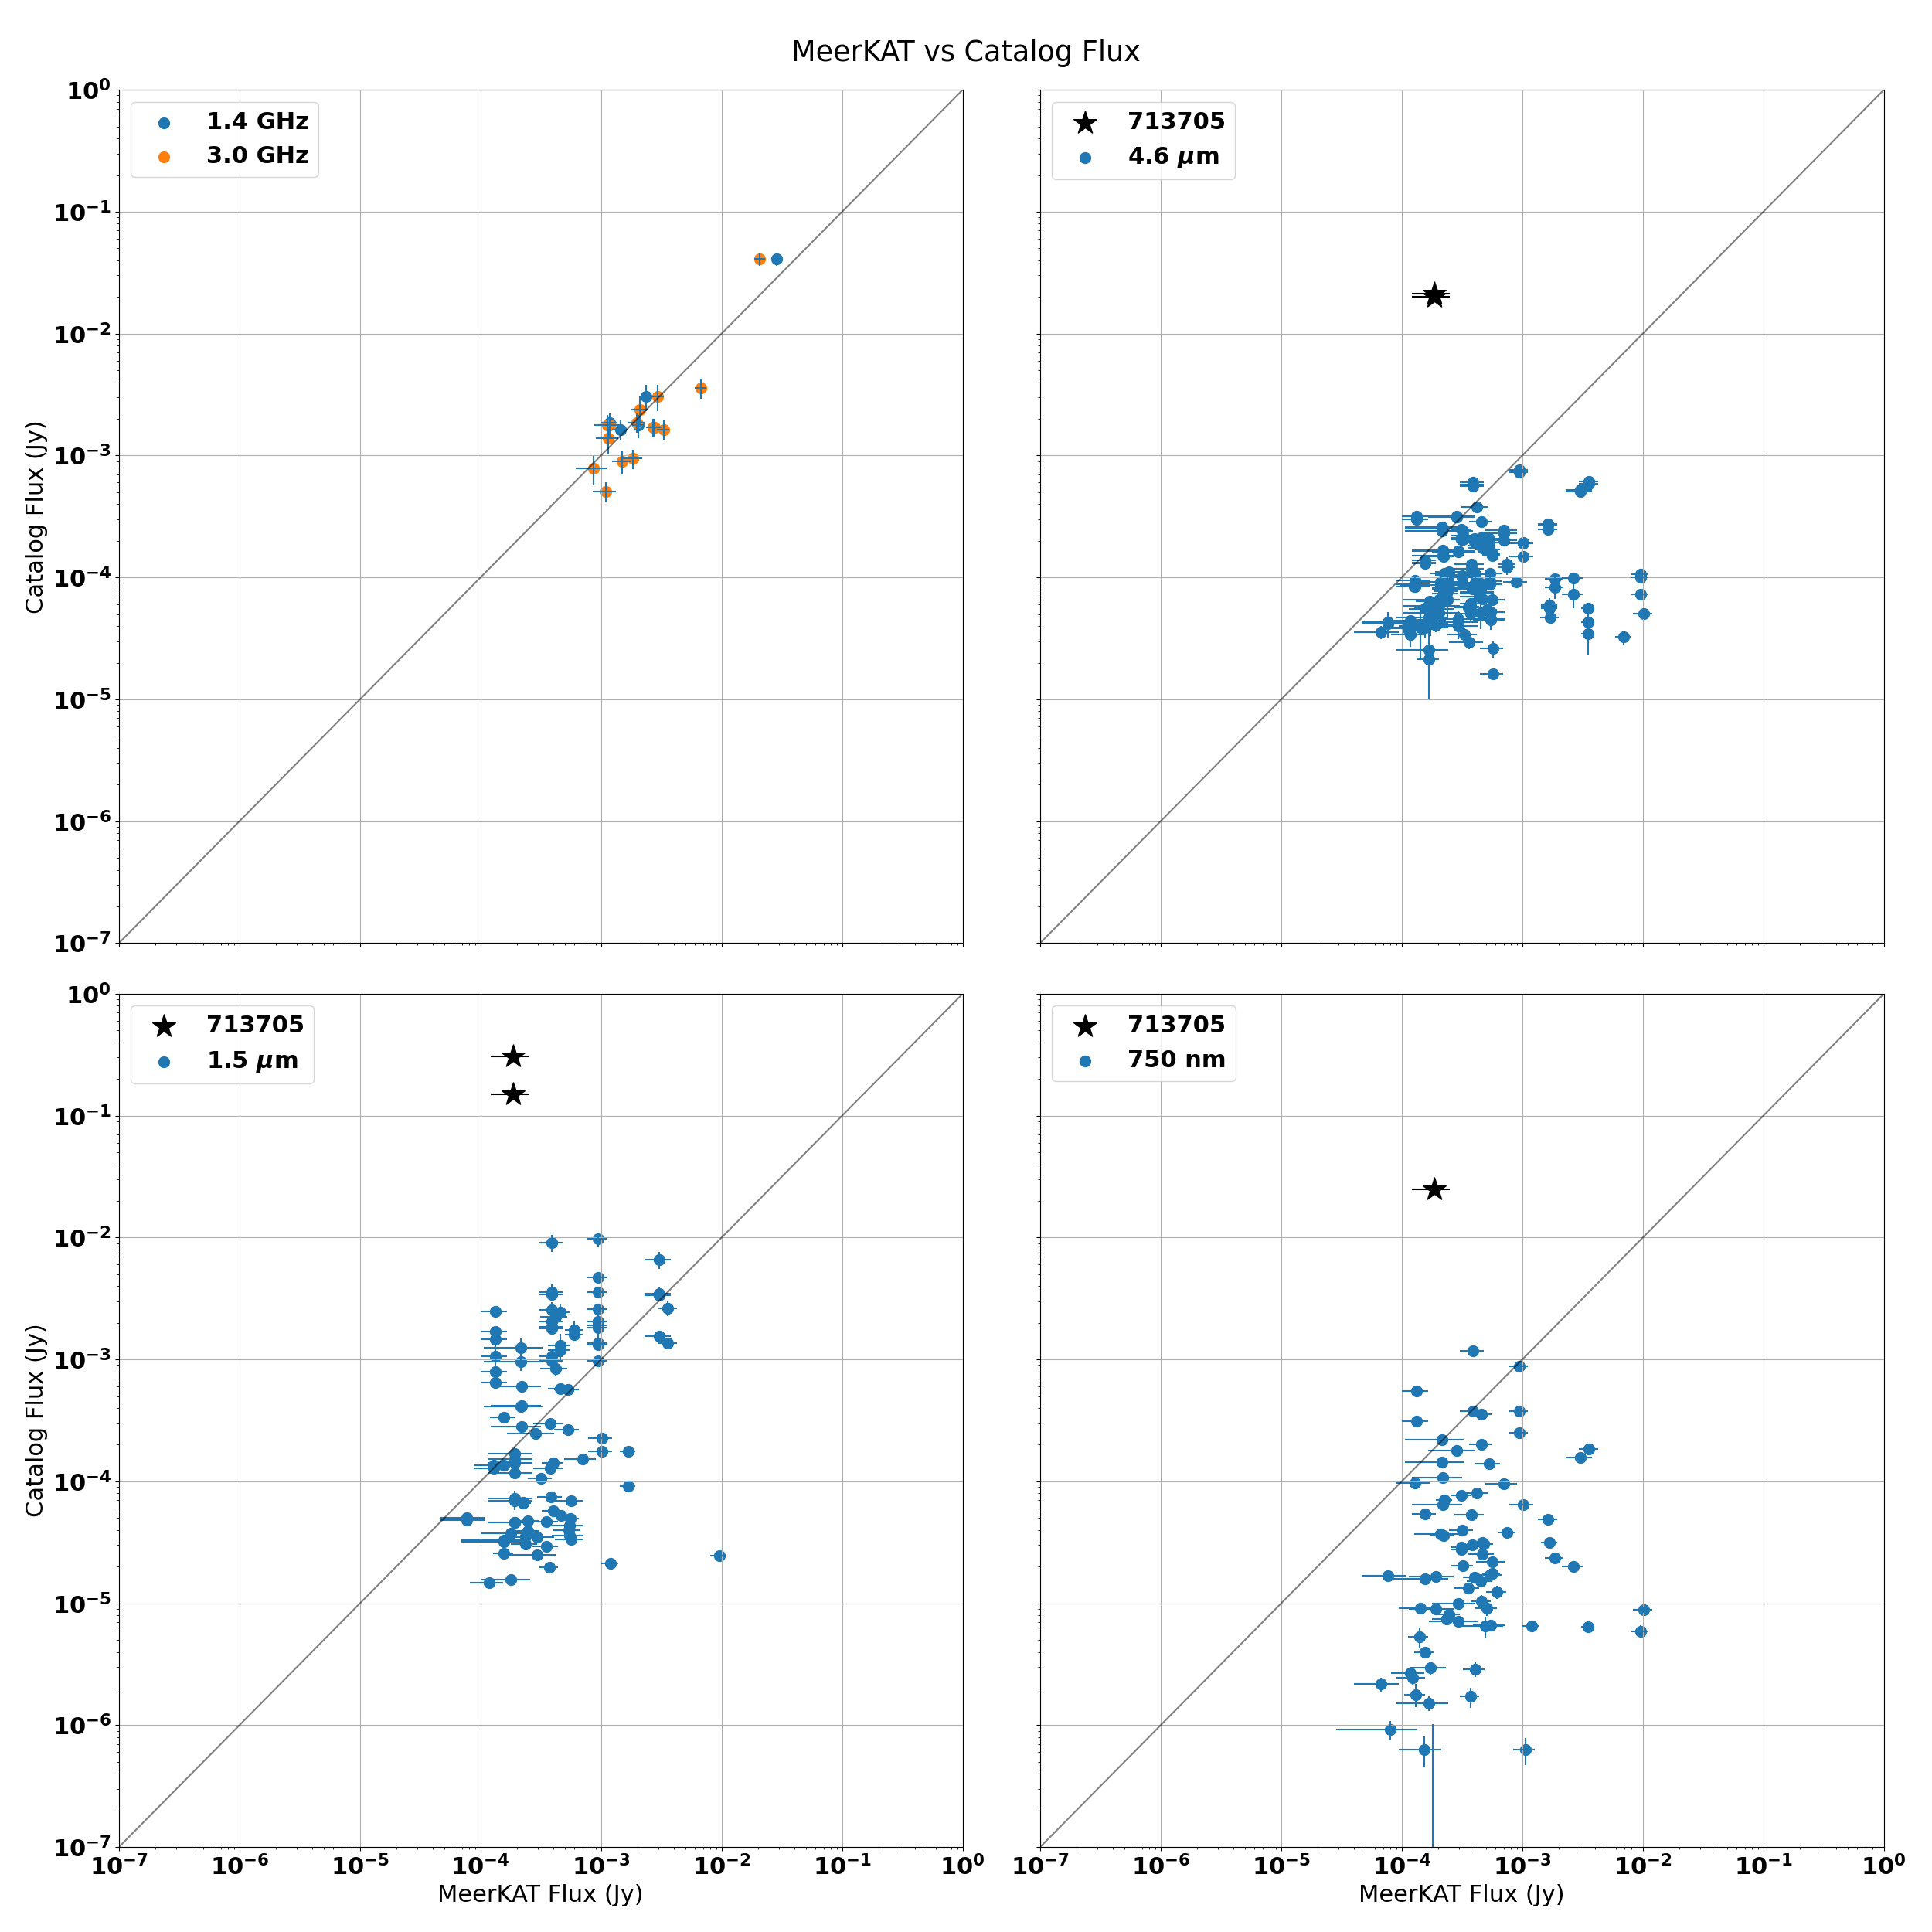
\includegraphics[width=0.9\textwidth]{combinedfluxfluxplots.png}
	\caption{The average integrated flux measured in MeerKAT images on the horizontal axis and the catalog flux at various wavelengths from a variety of different catalogs are shown on the vertical axis. Source 713705 is a clear outlier and is highlighted with a black star symbol. The catalogs used are listed in the Acknowledgments section.}
	\label{fig:combinedfluxfluxplots}
\end{figure}

\begin{figure}
	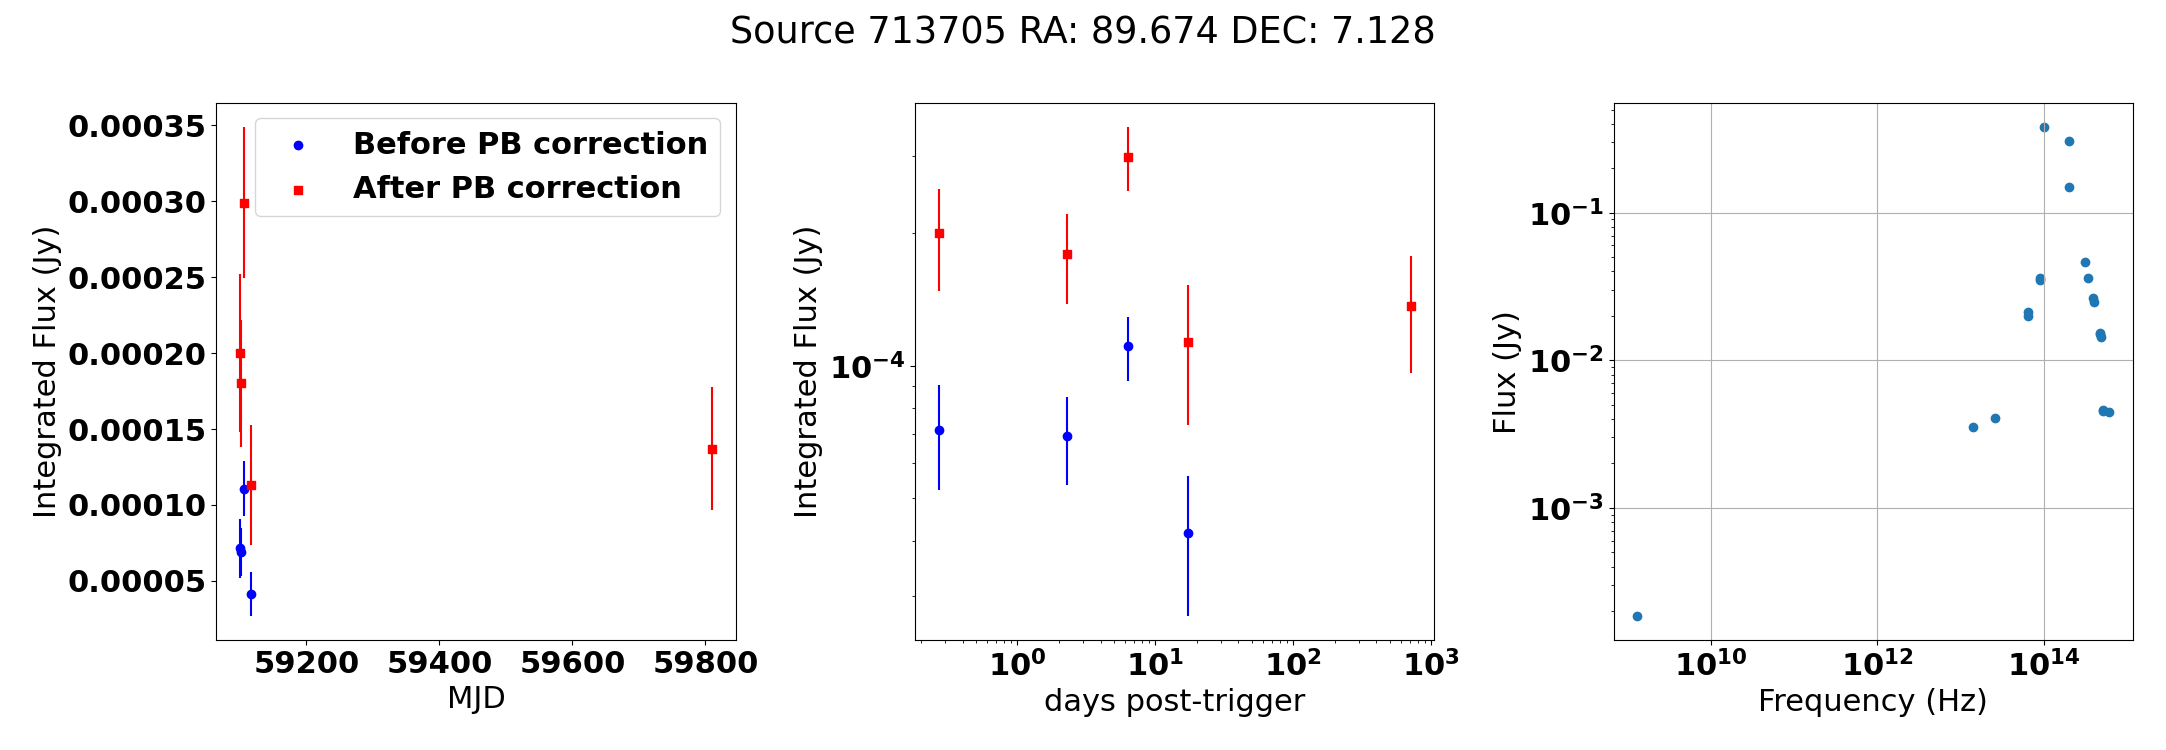
\includegraphics[width=\textwidth]{src713705lc4.png}
	\caption{Light curve and spectral energy distribution for source 713705, for which the optical counterpart is classified as a giant. The left panel shows the light curve on a linear scale, the middle panel the light curve on a log-log scale (with the start time being the trigger time of the GRB in the field), and the right panel is the spectral energy distribution with measurements from \citet{2003yCat.2246....0C,2012wise.rept....1C,2022yCat.1355....0G} as a part of the catalogs searched in this work.}
	\label{fig:src713705lc4.png}
\end{figure}

\begin{figure}
	% 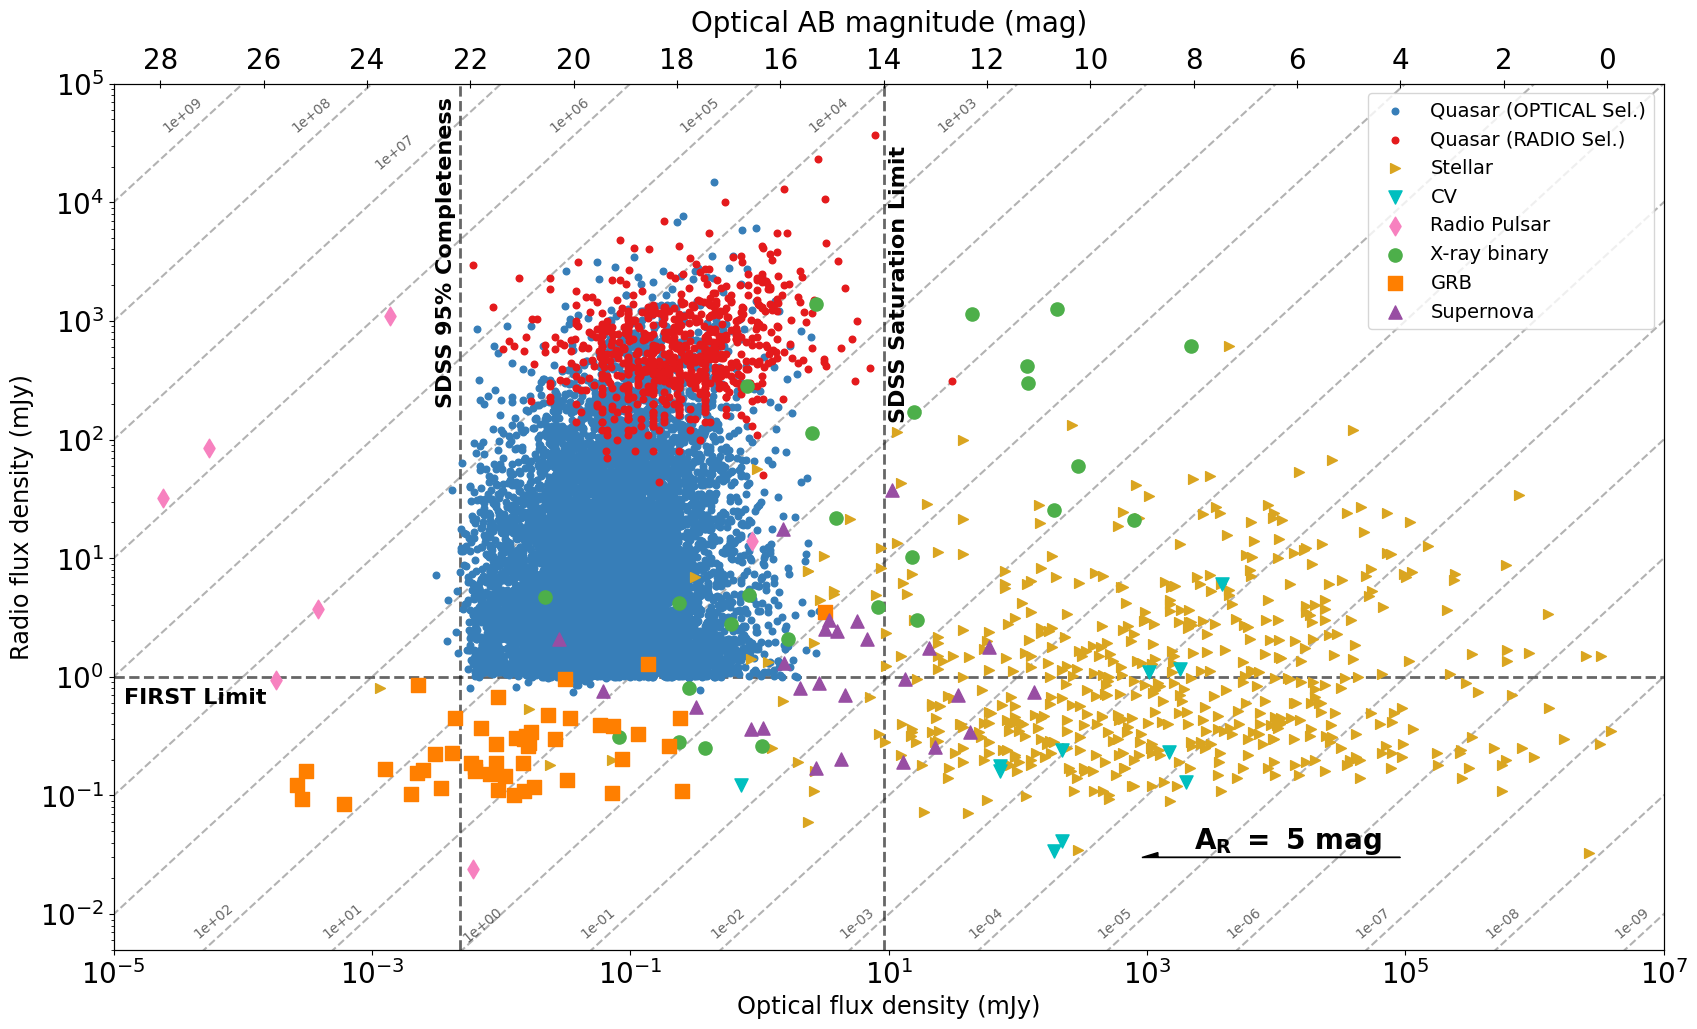
\includegraphics[width=0.9\textwidth]{ro_figure_1.png}
	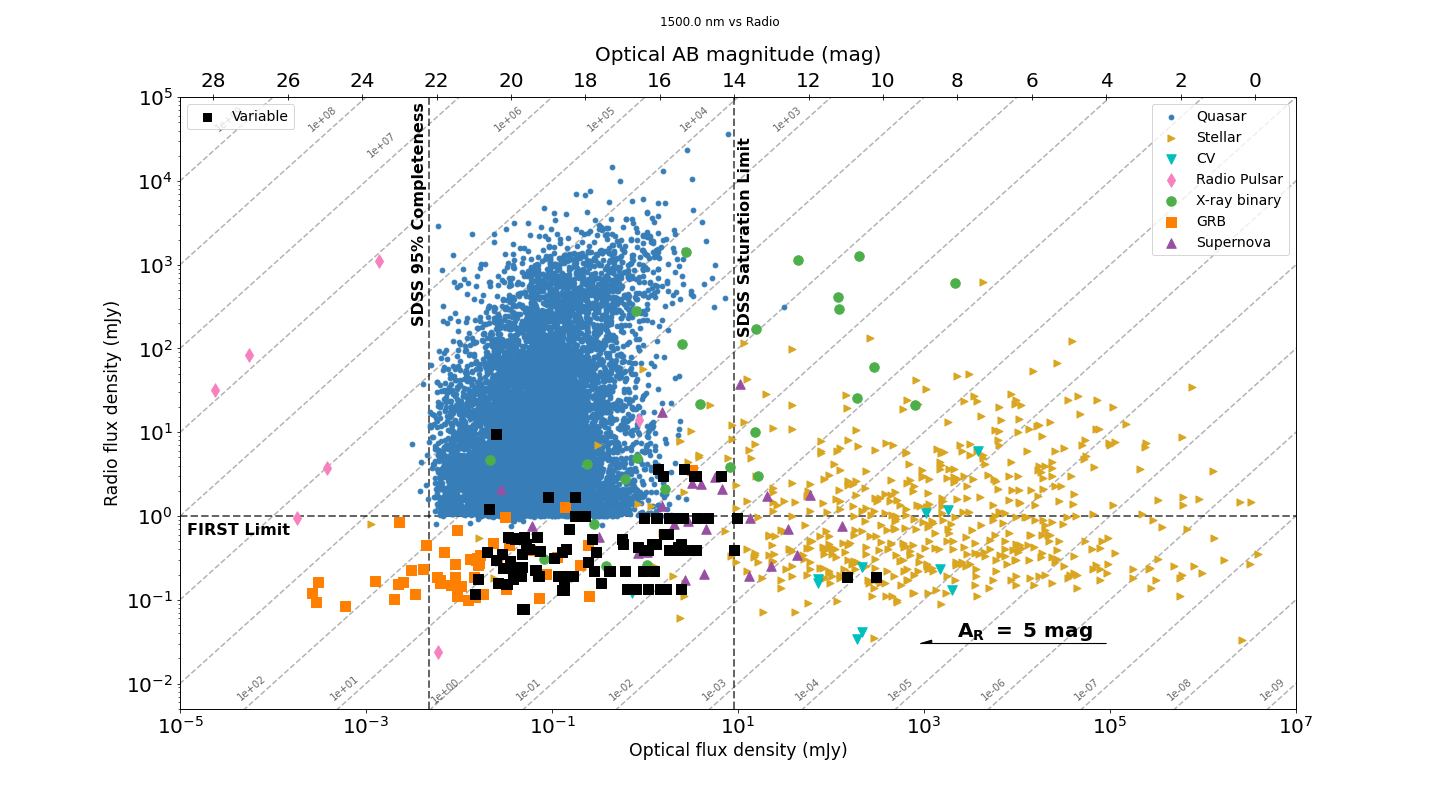
\includegraphics[width=\textwidth]{radio_opt_1500.0.png}
	\caption{A plot from~\citet{2018MNRAS.479.2481S} showing radio vs optical (or near-infrared) flux density of a variety of variable sources with the fluxes of the catalog matched sources at $1500$ nm overplotted in black squares. Catalog matched fluxes are from~\citet{2003yCat.2246....0C,2006AJ....131.1163S,2013Msngr.154...35M,2007MNRAS.379.1599L}.}
	\label{fig:stewartetalplot}
\end{figure}


\subsubsection{Variable Source Characteristics}
Figure~\ref{fig:combinedfluxfluxplots} shows the average flux of our variable sources in the MeerKAT observations plotted on the horizontal axis and the associated catalog flux on the vertical axis. The matching catalog radio sources are close in flux to the averaged measured flux in MeerKAT. The proximity of the points to the 1:1 diagonal line shows how well they correspond. At other wavelengths, the flux does not appear to follow any specific correlation, but instead appears to be a cluster of sources with an outlier or two. These outliers are from a single source, source 713705 as identified in our TraP runs, that is classified as a star in multiple catalogs (light curve shown in Figure~\ref{fig:src713705lc4.png}). 

We also see this outlier source in Figure~\ref{fig:stewartetalplot}, where we have overplotted our variable sources with associations on the radio-optical classification from \citet{2018MNRAS.479.2481S}. From this figure, it is clear that our outlier is within the stellar sources, while the other sources are near the active galactic nuclei (AGN) and stellar explosions within this radio-optical parameter space. The other variables are very likely not supernovae or GRBs since they are variable sources over timescales that are characteristic of AGN and not supernovae or GRBs. Further catalog information about the outlier source from the TESS catalog version 8.2 gives the luminosity class of this source to be a giant. Two additional sources are classified as stars and have a luminosity class of dwarf. Eleven additional sources are classified as stars in the TESS 8.2 catalog, Guide Star Catalog 2.4.2, Dark Energy Survey Data Release 2, and Sloan Digital Sky Survey 16. In these same catalogs, 52 sources are either classified as extended sources or have multiple sources matched within the 1 arcsecond search radius. 


\subsection{Discussion}
\label{sec:discussion}
Although there were no confidently detected transients, there remain a large number of variable sources that warrant further investigation. In addition, the lack of transient detections can be used to constrain parameter space via transient simulations. As part of further investigation of these sources, the nature of the variability, whether it is intrinsic or extrinsic variability, is examined here.

\begin{figure}
	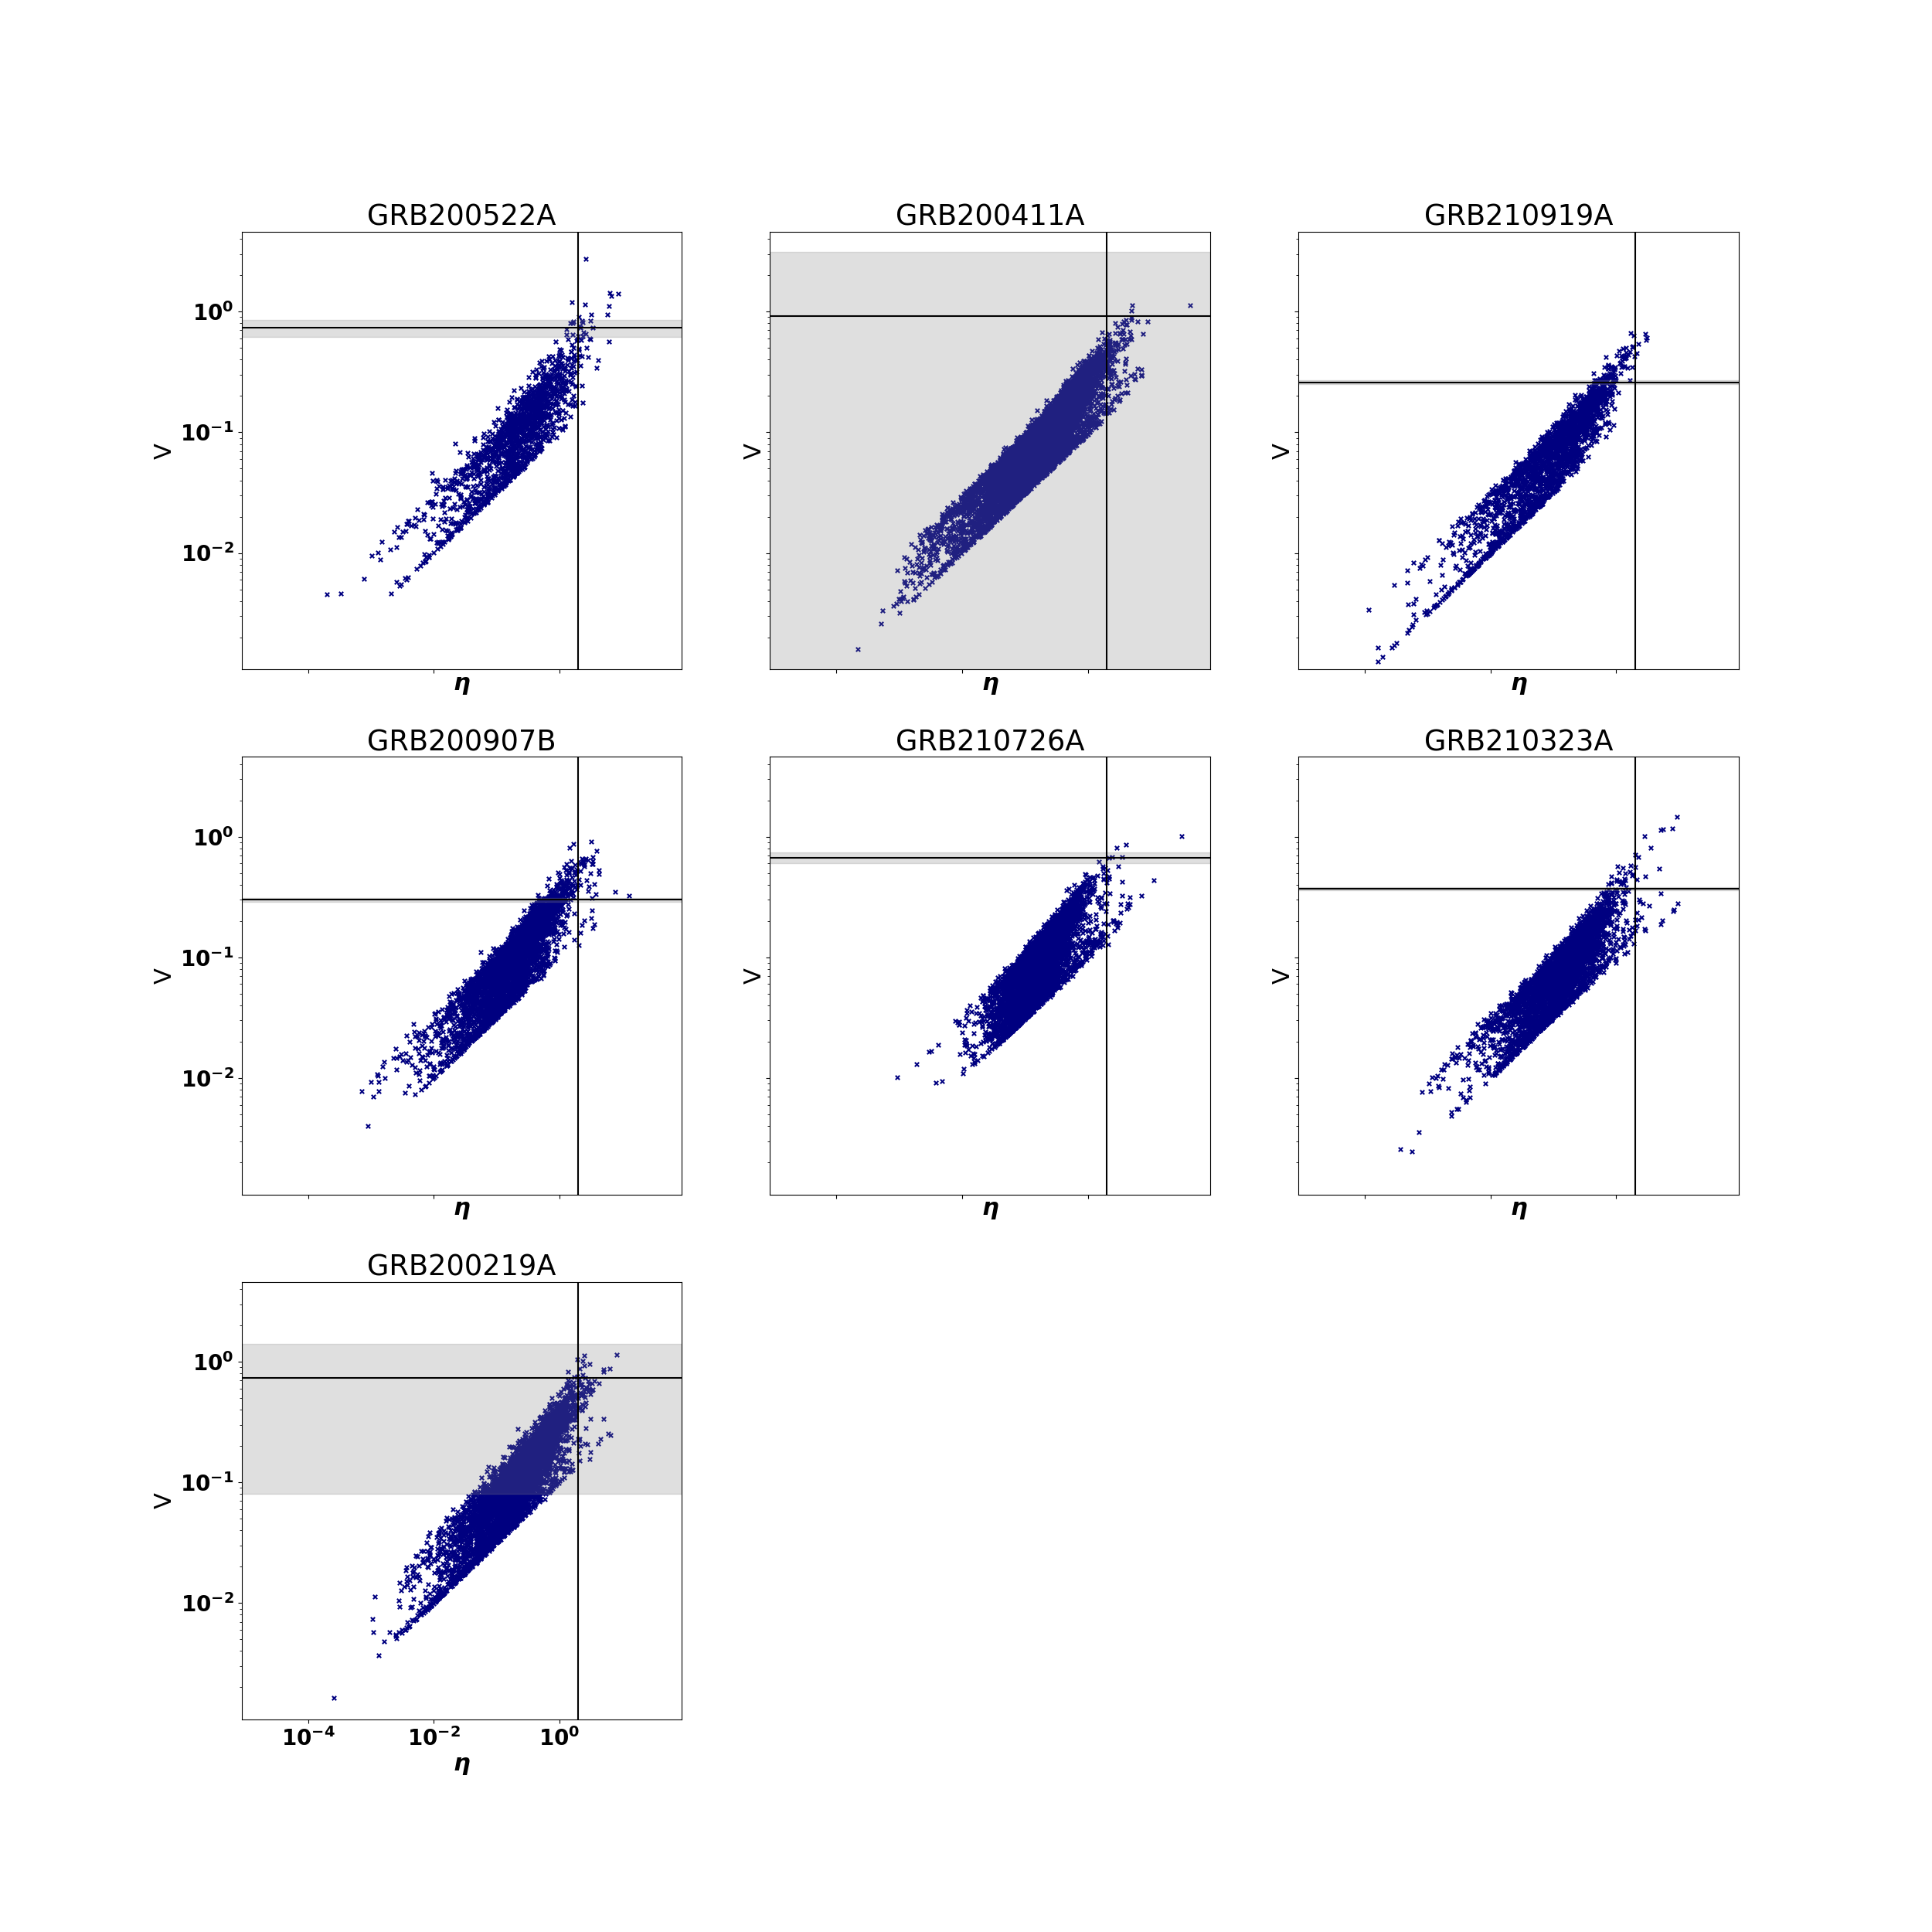
\includegraphics[width=\textwidth]{allfieldsvar.png}
	\caption{Scatter plot showing $V-\eta$ for each field with $\eta=2$ as a vertical line and the modulation index with errors from Table~\ref{tab:sciprop} shown as a horizontal line with a grey shaded region. The modulation index is defined similarly to the variability metric $V$ and is shown for comparison. The title of each subplot indicates the field that the sources are within.}
	\label{fig:allfieldsvar}
\end{figure}

\begin{figure}
	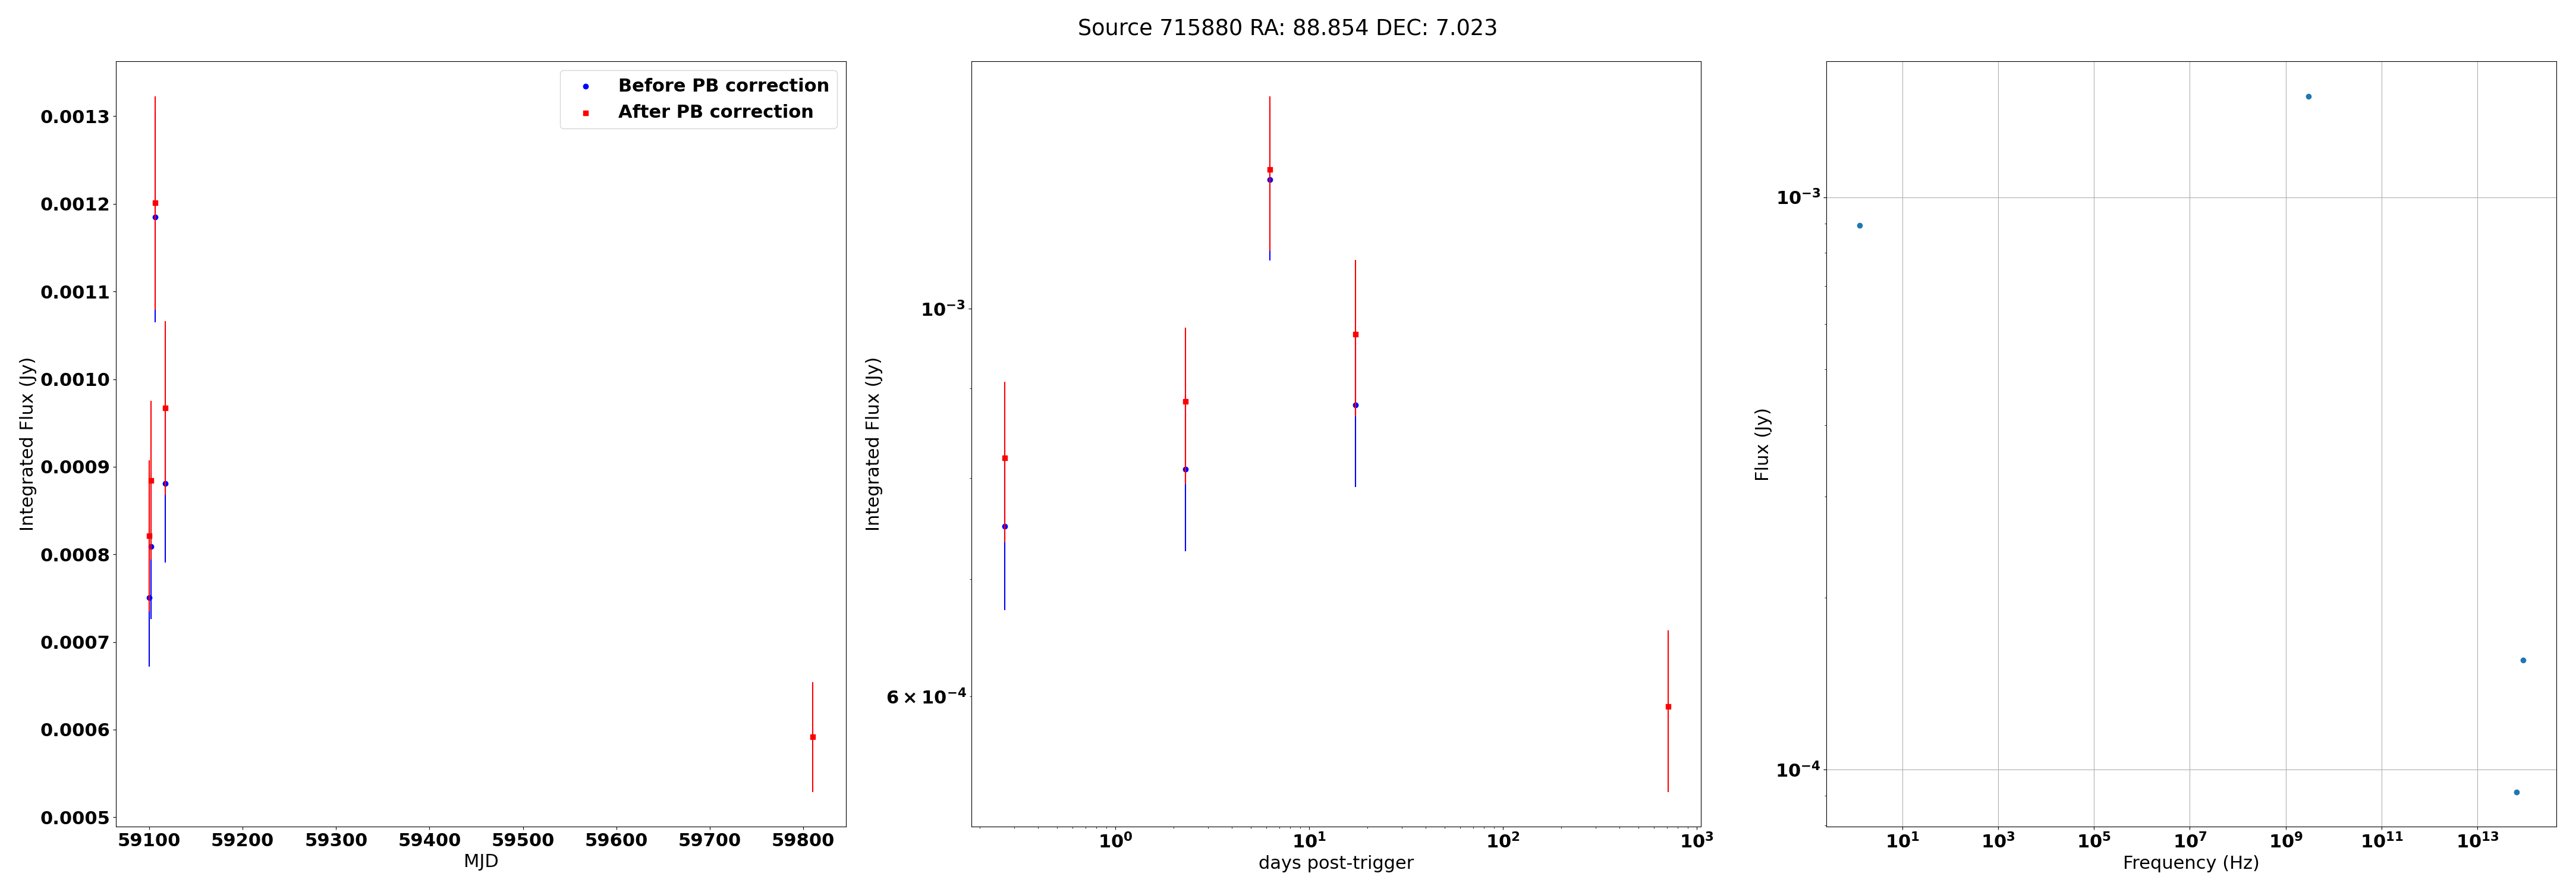
\includegraphics[width=\textwidth]{src715880lc4.png}
	\caption{Light curve and spectral energy distribution for source 715880. The left panel shows the light curve on a linear scale, the middle panel the light curve on a log-log scale (with the start time being the trigger time of the GRB in the field), and the right panel is the spectral energy distribution from \citet{2008AJ....136..735L}  as a part of the catalogs searched in this work.}
	\label{fig:src715880lc4.png}
\end{figure}

\subsubsection{Scintillation Effects}
Interstellar scintillation is a known cause of variability in the radio sky. \citet{1998MNRAS.294..307W} provides some background on the kinds of variability expected from radio observations. Scintillation can occur when light at radio wavelengths interacts with inhomogeneities in the ionized component of the interstellar medium. The scattering produced by this interaction can be described as being either ``weak'' or ``strong.'' The dividing line between these regimes can be determined by comparing the observing frequency with the transition frequency $\nu_0$. When the observing frequency is approximately $\nu_0$, the modulation index, defined as $\sigma/\mu$ or the fractional variation in flux where $\mu$ is the average flux and $\sigma$ is the variation in flux, is equal to one. If the observing frequency is greater than the transition frequency, the observations are in the weak scattering regime, and if it is less than the transition frequency, the observations are in the strong scattering regime. Given the observing frequency of 1.3~GHz and typical $\nu_0$ values shown in Table~\ref{tab:sciprop}, all the observations in this survey are in the strong scattering regime. The strong scattering regime can be further broken down into refractive and diffractive scintillation. For all the timescales involved in these variable sources we are interested in examining refractive scintillation. ~\citet{2019arXiv190708395H} created models of refractive scintillation using $H_{\alpha}$ maps. Using these models and relations, we find that we expect scintillation to have a large effect on the amount and kinds of variability to expect in the light curves of individual sources. 


\newgeometry{margin=1.25in} % modify this if you need even more space
\begin{landscape}
	\begin{deluxetable}{lllllllll}
		\tablecolumns{9}
		\tablewidth{0pc}
		\tablecaption{Observed fields and some properties, together with the scintillation parameters calculated from~\citet{2019arXiv190708395H} for the center of each field. \label{tab:sciprop}}
		\tablehead{\colhead{Field Name}& \colhead{Average Noise}  &  \colhead{\# of variable sources} &  \colhead{Survey length}  &  \colhead{$\nu_0$} &   \colhead{m} & \colhead{t$_{var}$}  \\
			\colhead{}& \colhead{($\mu$Jy/beam)} &\colhead{} & \colhead{(days)} &\colhead{ (GHz)} & \colhead{}& \colhead{(days)}\\}
		\startdata
		GRB200219A &                   9 &                     17 &                  8.1 &      2.2 & $0.74\pm0.66$ &      $1.7\pm4.5$ \\
		GRB200411A &                   7 &                     51 &                  6.2 &      1.5 & $0.92\pm2.22$ &      $0.9\pm6.5$ \\
		GRB200522A &                  31 &                      4 &                 14.0 &      2.2 & $0.74\pm0.12$ &      $1.6\pm0.8$ \\
		GRB200907B &                  12 &                     14 &                 17.2 &     10.9 &  $0.3\pm0.01$ &     $57.9\pm4.7$ \\
		GRB210323A &                   9 &                     12 &                189.6 &      7.5 & $0.37\pm0.01$ &     $23.7\pm2.4$ \\
		GRB210726A &                   9 &                     24 &                151.7 &      2.7 & $0.67\pm0.07$ &      $2.1\pm0.6$ \\
		GRB210919A &                  18 &                      0 &                  7.2 &     14.2 & $0.26\pm0.01$ &     $62.4\pm4.1$ \\
		\enddata
	\end{deluxetable}
\end{landscape}
\restoregeometry
 \doublespacing
Table~\ref{tab:sciprop} shows a summary of all the fields in the survey, some of their properties, and the scintillation parameters calculated from~\citet{2019arXiv190708395H}. A closer look at this table may explain a large amount of the variability we see in our survey. For example, the field with the most transient detections, the GRB 200411A field, has a transition frequency $\nu_0$ that falls within the observing band. Consequently, the modulation index m is quite high for this field. Combining this information with the variability timescale $t_{var}$ reveals that in principle all the variables in this field can be explained by refractive scintillation. There are other fields in which $\nu_0$ is close to the observing band: using the same logic as for the GRB 200411A field, we can say that the variables in the GRB 200219A field, GRB 200522A field, GRB 210323A field, and GRB 210726A field can be explained by refractive scintillation. Note that the number of detected variables in the GRB 200522A field is lower due to the higher average noise. Any variable in the aforementioned fields would need to show a calculated modulation index greater than the already high expected modulation index from scintillation in these fields, and after examining these sources none of them have a modulation index significantly higher than that predicted for refractive scintillation. In Figure~\ref{fig:allfieldsvar}, we show how the modulation index, shown as a grey shaded region, compares to the variability parameter, V, in this scatter plot of $\eta$ and V for each field. This plot shows how for some fields, the modulation index is very high, and could be consistent with all of the sources in the field. Note, however, that this does not consider timescale of variability.

In the case of the GRB 210919A field, we see that the predicted scintillation timescale is much longer than the duration of the survey of this field. Therefore, it follows that no variables were detected. However, in the GRB200907B field, we also see a longer timescale for scintillation than the length of the survey, and in this field there are detected variable sources. All but two of the sources have variability timescales that are at least 17 days, as can be seen in source 715880 shown in Figure~\ref{fig:src715880lc4.png} and in source 713705 in Figure~\ref{fig:src713705lc4.png}. A possible explanation for this timescale and modulation index could be that the scattering screen is closer than is assumed in the estimates for scintillation. This possibility could be supported by the estimations on the refractive scintillation from~\citet{2019arXiv190708395H} showing one source that is very different in modulation index and timescale. This source ended up having variability more consistent with modulation indices and timescales like the rest of the field. Therefore, for this study, we took a single modulation index at the center of the field, but the point remains that there is a possibility that this region of the sky contains very inconsistent ISM charged particle populations that could possibly explain the variability.


\subsubsection{Intrinsic Variablity}
Of the fourteen variable sources in the GRB 200907B field, two have variability on timescales shorter than 15 days, a timescale inconsistent with extrinsic variability from refractive scintillation according to the models we have used, therefore this variability is most likely intrinsic to these sources. Source 713705, also discussed in the previous section, is a known variable star also called ASASSN-V J055841.70+070741.7, with a period of 17.22 days reported in the AAVSO International Variable Star Index~\citep{2006SASS...25...47W}. This source is known to be variable at other wavelengths and could be intrinsically variable in the radio as well. The light curve for this source is shown in Figure~\ref{fig:src713705lc4.png}. The variability of this source is quite short with the flux rising to its peak and falling again within a timespan of about 15 days. Like source 713705, source 715880 shows a single high flux measurement in a fifteen day span which can be seen in Figure~\ref{fig:src715880lc4.png}. This source is not classified in any other catalogs, but has some flux measurements in the infrared with WISE~\citep{2014yCat.2328....0C}. Figure~\ref{fig:transphasespace} shows source 715880 with its variability timescale (assuming 15 days) multiplied by the observing frequency (1.3 GHz), against its luminosity. Two values are shown on the scatter plot for this source: one if the source is at 10 kpc and on if the source is at 10 Mpc. From this plot, we see that the source is possibly an X-ray binary or nova if it is at 10 kpc, and it is possibly a supernova if it is at 10 Mpc. Further investigation into this source, including follow-up observations, are warranted to classify the source and determine what sort of variability could cause its radio behaviour.

\begin{figure}
	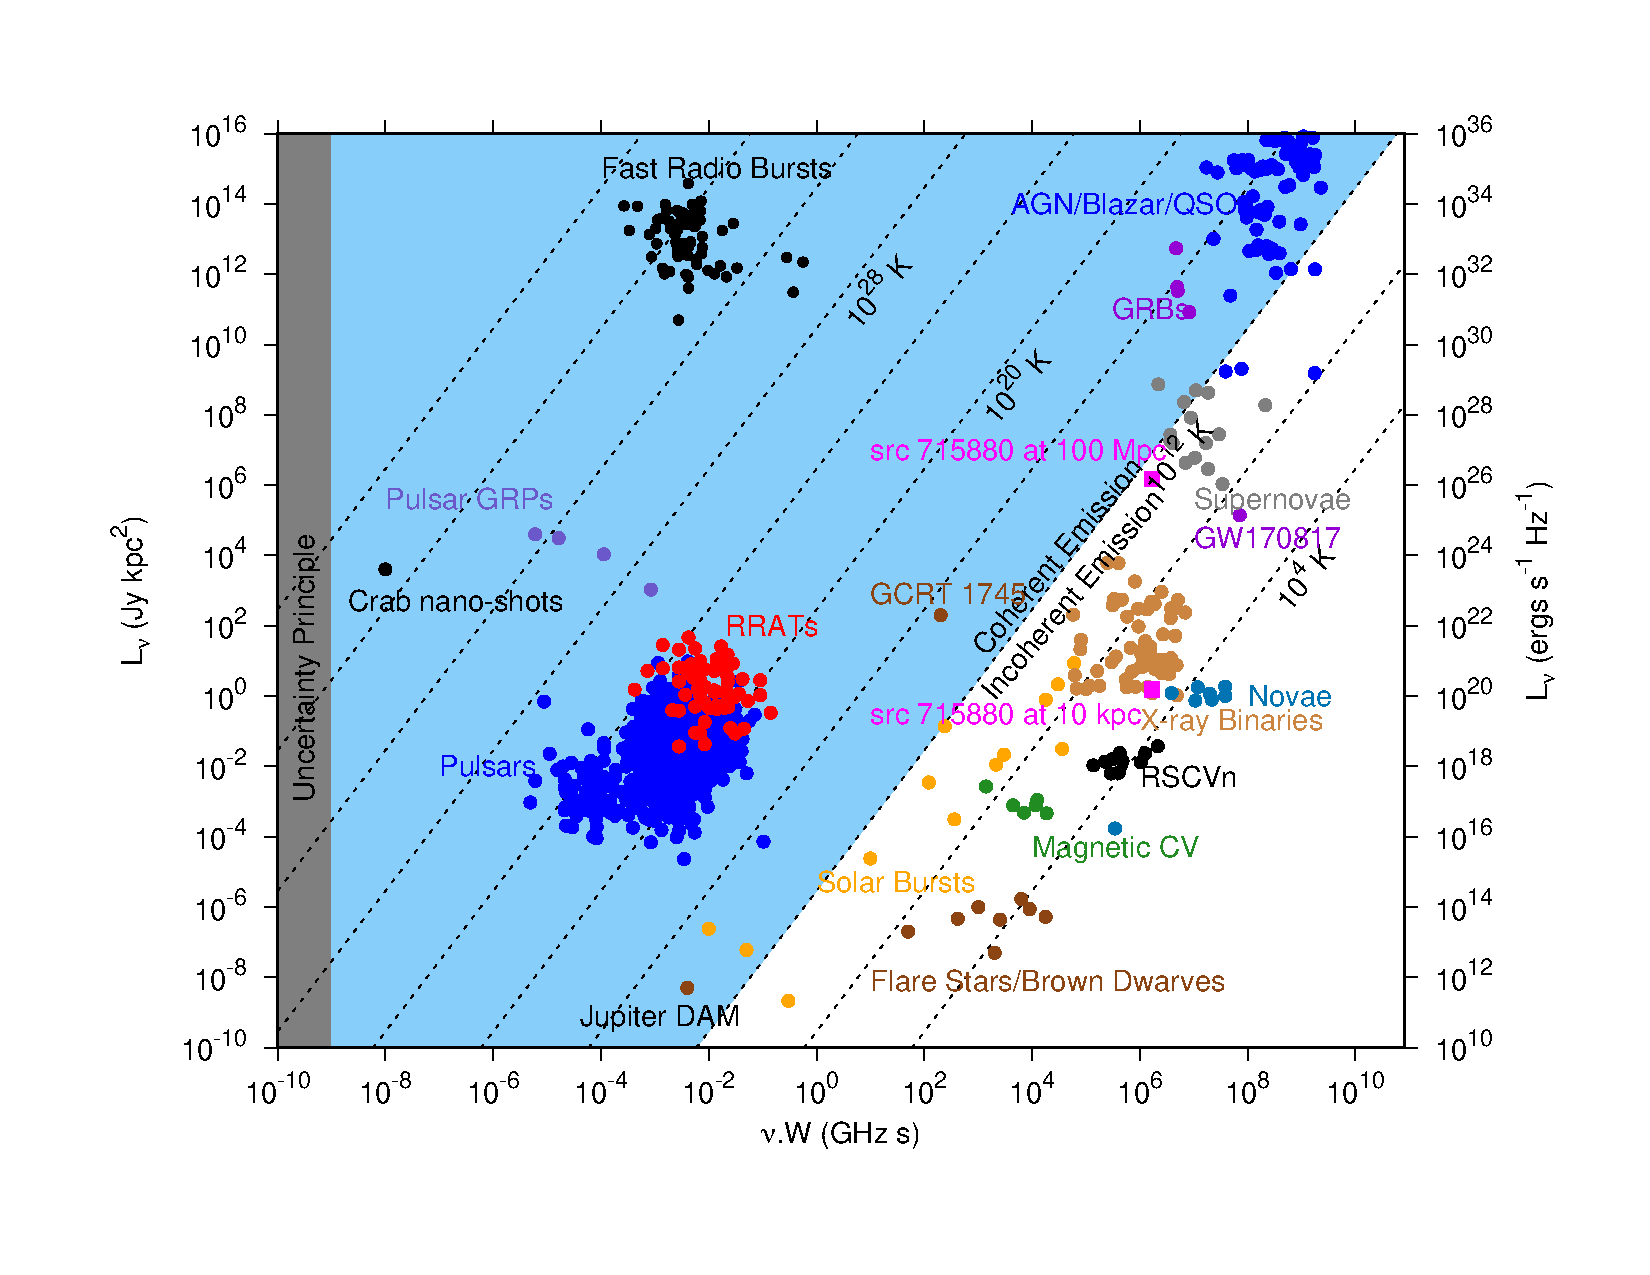
\includegraphics[width=0.9\textwidth]{phase_space_ewass.pdf}
	\caption{Scatter plot of a variety of transients observable in radio as a function of variability timescale and luminosity, adapted from~\citet{2015MNRAS.446.3687P}. Overplotted with pink squares are the values for source 715880 at both 10 kpc and 10 Mpc.}
	\label{fig:transphasespace}
\end{figure}
% \newgeometry{margin=1.25in} % modify this if you need even more space
\begin{landscape}
\begin{figure}
	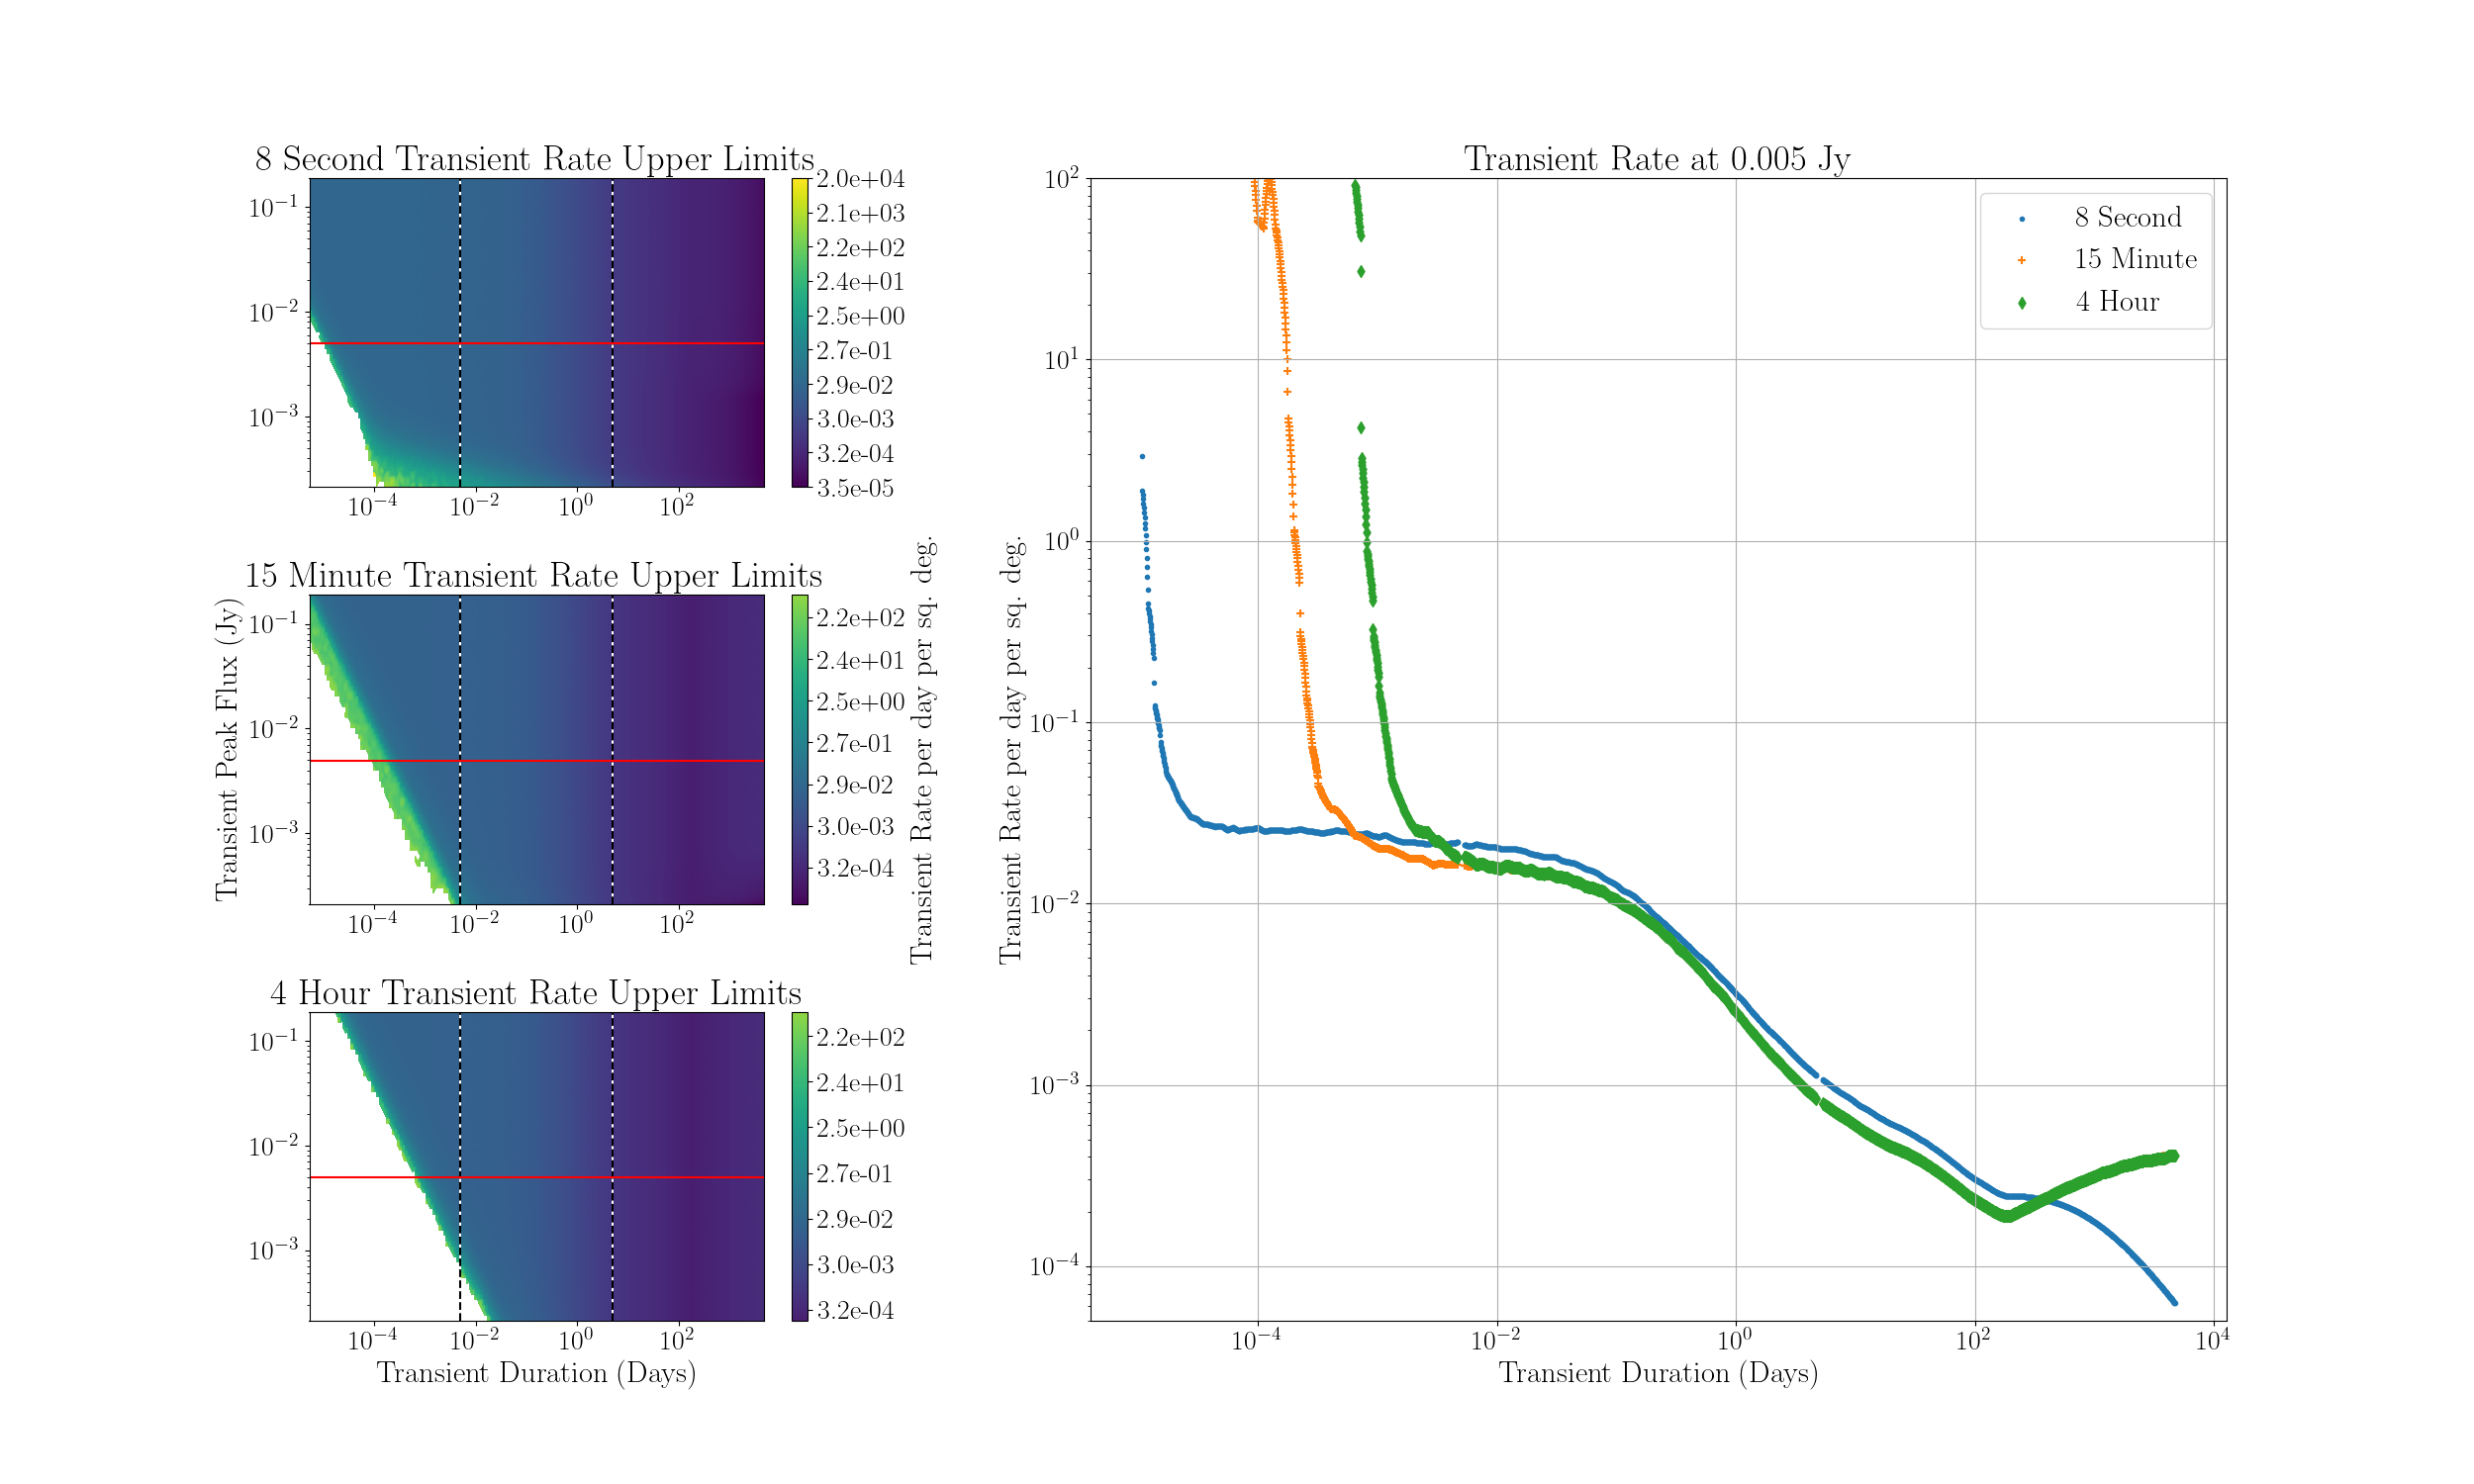
\includegraphics[width=1.1\textwidth]{allplots.png}
	\caption{Transient rate upper limits for our survey based on the 8-second, 15-minute and 4-hour observations, calculated using the simulations code of ~\citet{2022ascl.soft04007C}. The left three panels show the transient rate upper limits color coded as a function of peak flux and duration. The panel on the right shows the transient rate as a function of duration at a given flux of 5 mJy, for the three different types of observations in our survey. Note that the dip downwards in upper limits on the 8 second timescale at long transient durations (approximately 100 days) is due to false transient detections and should be ignored.}
	\label{fig:threelimits}
\end{figure}

\begin{figure}
	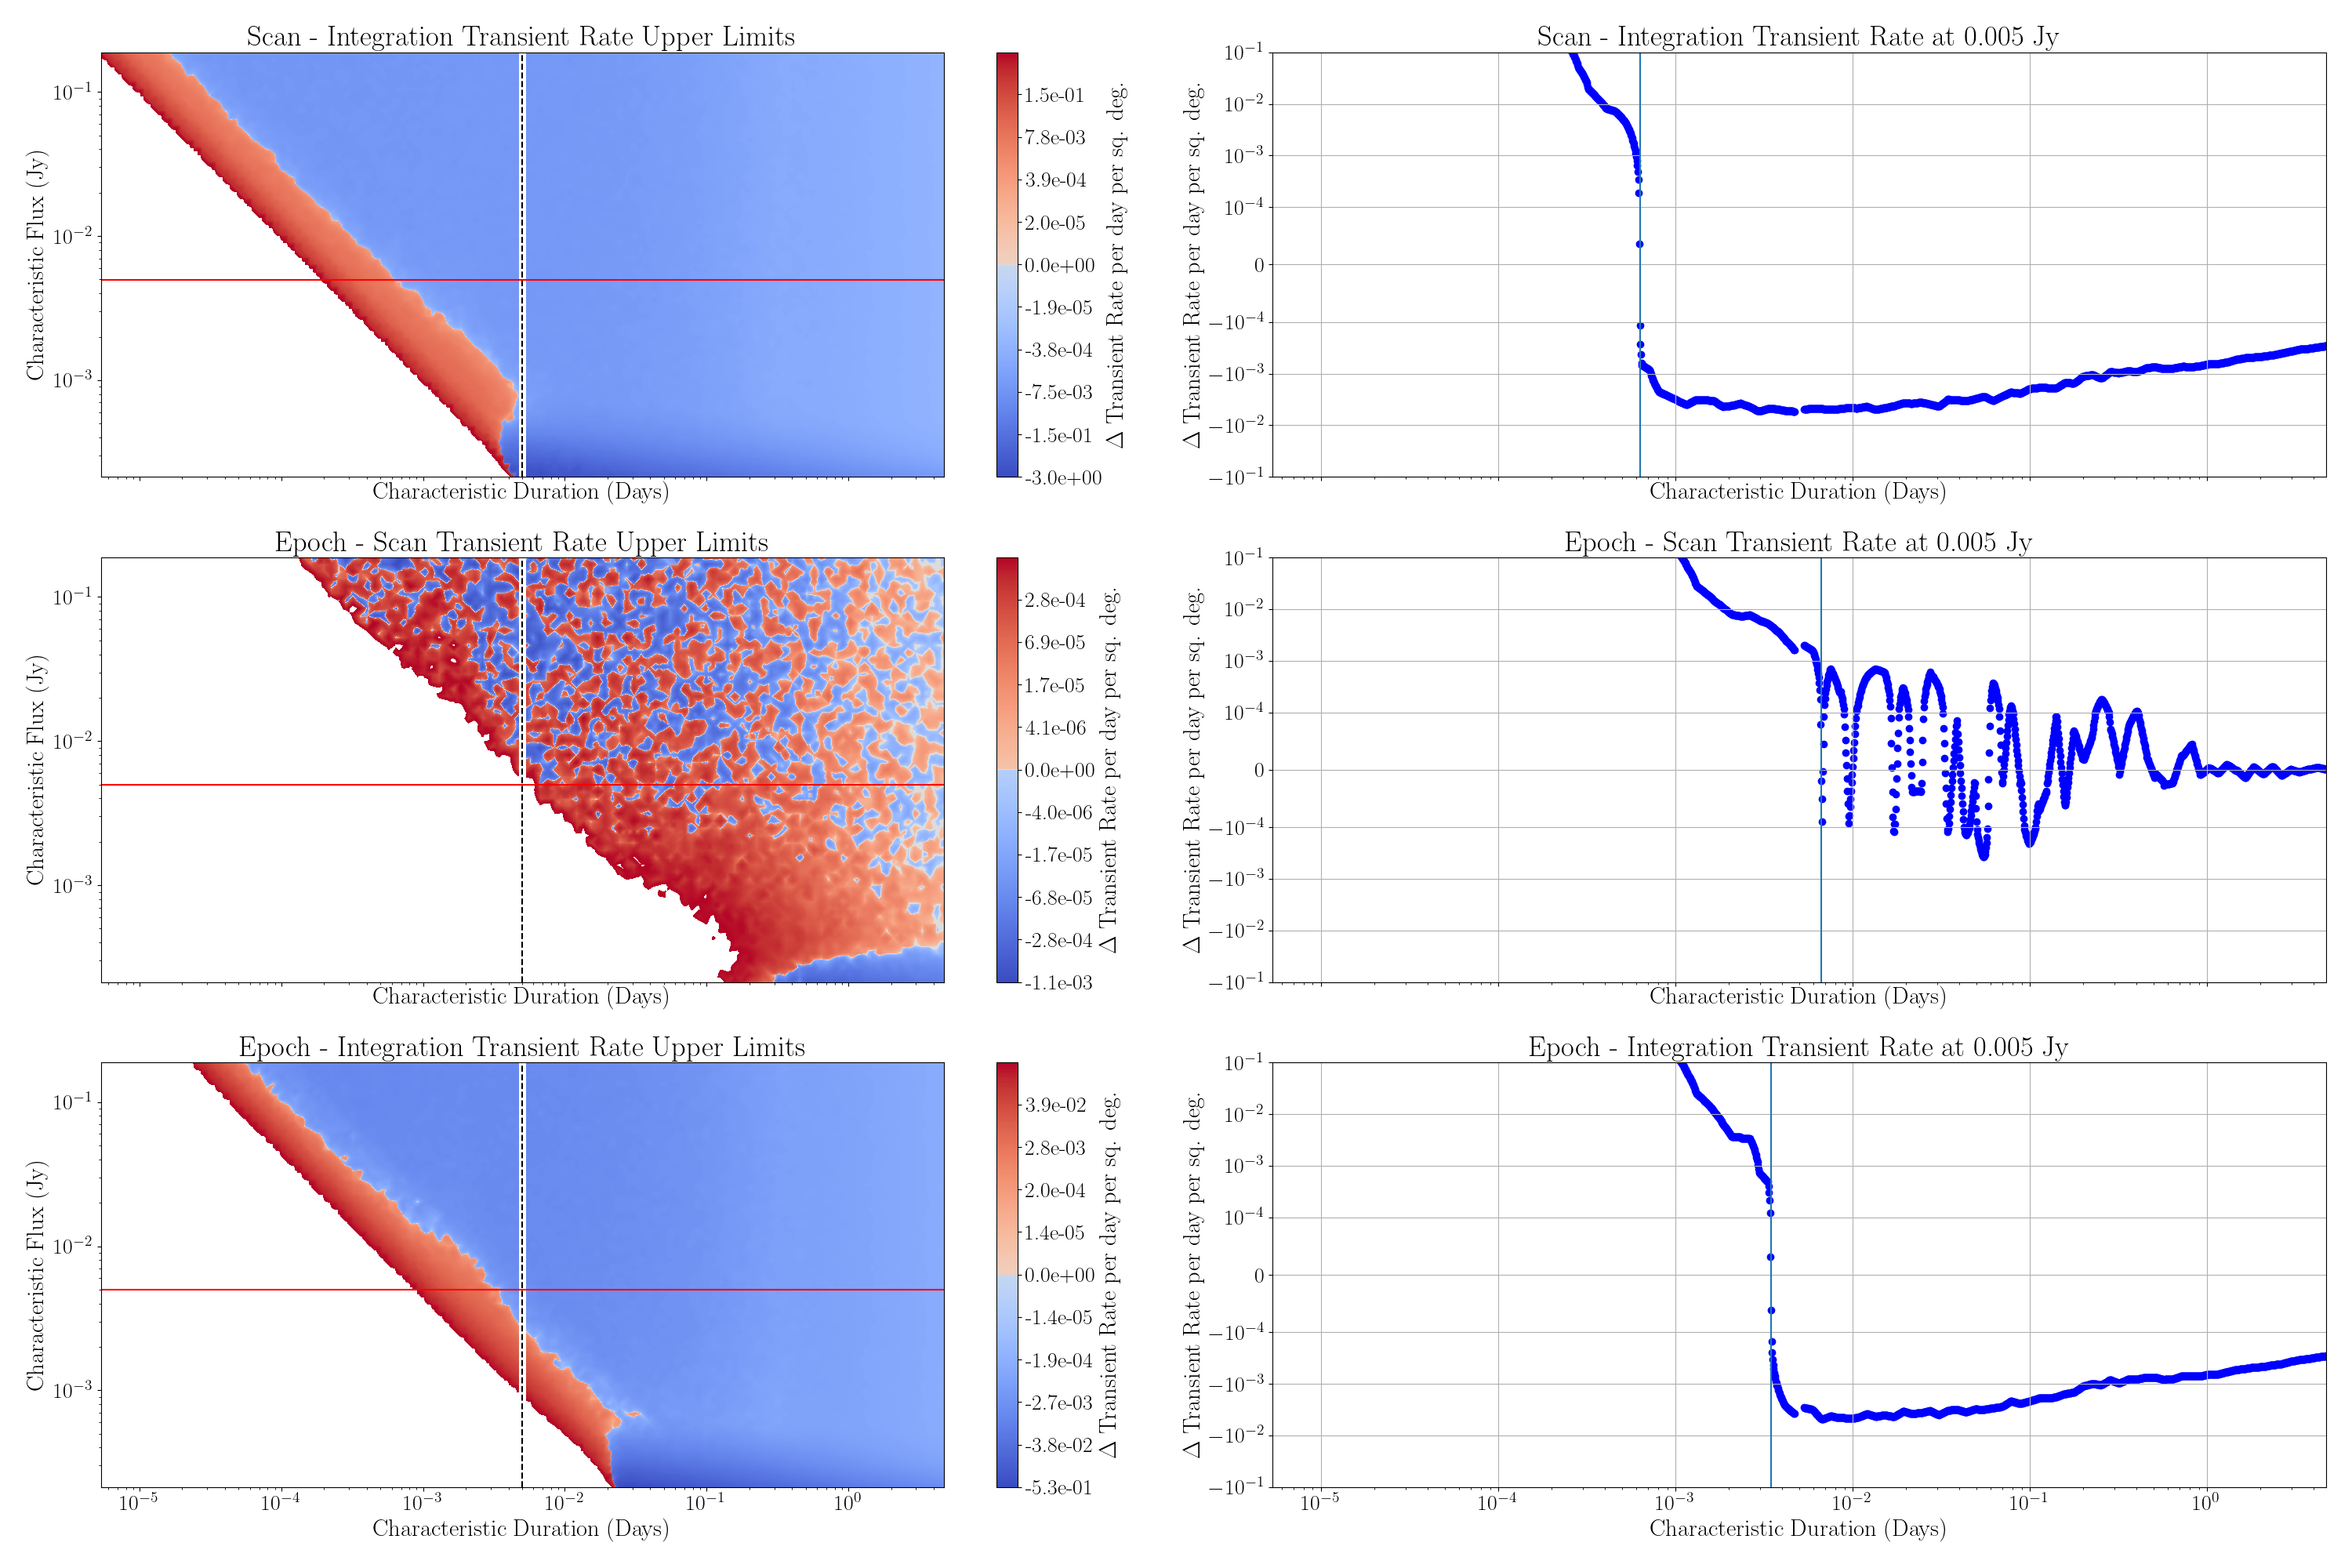
\includegraphics[width=1\textwidth]{diffplots.png}
	\caption{Difference in transient rate upper limits, calculated using the simulations code of ~\citet{2022ascl.soft04007C}, between the three different timescales of the survey. The left three panels show the differences between transient rate upper limits color coded as a function of flux and duration. The three right panels show this difference as a function of duration at a given flux of 5 mJy. The region that favors each timescale is noted by the corresponding color (red or blue) and the sign (positive or negative).}
	\label{fig:threediff}
\end{figure}

\end{landscape}
\restoregeometry
 \doublespacing
\subsubsection{Transient Rate Limits}
Calculating transient rates is a key way to characterize transients and compare the sensitivity of surveys like this one to other surveys in various parts of transient parameter space. Transient rates are often calculated by assuming that transients are distributed as Poisson distributions and the rate is calculated by determining the number of detections over the duration of the survey. However, as discussed in~\citet{2017MNRAS.465.4106C} and~\citet{2016MNRAS.459.3161C}, many observational effects are often ignored, such as gaps within a survey or within individual observations, which leads to estimated transient rates that are off by orders of magnitude. Therefore, in order to place accurate limits on the transient rate imposed by the survey presented here, we use the transient simulations~\citep{2022ascl.soft04007C} as described in detail in~\citet{2022A&C....4000629C}. 

In Figure~\ref{fig:threelimits}, the transient rate upper limits are shown for the 8-second, 15-minute, and 4-hour images. The left panels show the transient duration on the horizontal axis, transient peak flux on the vertical axis, and the transient rate upper limit in the color axis. The right panel shows the transient duration on the horizontal axis and the vertical axis shows the calculated transient rate for a transient with a flux density of 5 mJy. Because these timescales all probe the same field, we can show them all in the same panel on the right by just taking the strictest upper limits on transient rates from each timescale. Note that the dip downwards in upper limits on the 8 second timescale at long transient durations (approximately 100 days) is due to false transient detections and should be ignored. These types of false detections can be mitigated by looking for the long timescale transients in the deeper images.

We further examined which parts of transient parameter space are best probed by which timescale. Figure~\ref{fig:threediff} shows the difference in calculated transient rate for all combinations of the timescales. The panels on the left show the transient duration on the horizontal axis, the transient flux on the vertical axis, and the difference between the transient rate upper limits on the color axis. Since lower limits are better, the timescale with the lowest limits are noted with either a red or blue color corresponding to either positive or negative values of the equation noted in the title of each plot. The panels on the right side show the difference in transient rate on the vertical axis for a transient at a flux of 5 mJy with the duration on the horizontal axis. The top plots show the difference between the 8-second and 15-minute timescales; the middle plots show the difference between the 4-hour and 15-minute timescales, and the bottom plots show the difference between the 4-hour and 8-second timescales. The top and bottom plots appear to show a certain fluence where the timescale that gives the lower limits changes. The middle plot shows less of a difference between the two timescales, although judging from the transient durations where each timescale gives lower limits in the top and bottom plots, there appears to be a small region in which the transient rate upper limit is lowest in the scans. 

In order to compare our results with other surveys, we also calculated transient rates using this method for a survey similar to~\citet{2011ApJ...728L..14B}, in which a commensal transient search was performed on archival calibrator observations of 3C 286 spanning 23 years on a cadence that is approximately weekly or slightly better than weekly. We use the same sensitivity in our simulations as is used in their survey. For the observation dates, we only have the information on the day and no information on the duration, so we take the time to be at midnight and set the duration to be sometime between 1.75 minutes and 2.25 minutes. We set the field of view to be 1 degree across. Using this setup, we create Figure~\ref{fig:bowerandsaulall}, which we can compare to our survey results in Figure~\ref{fig:threelimits}. The transient flux that our survey is sensitive to is at least an order of magnitude deeper, and in the case of the 4-hour timescale even two orders of magnitude deeper. However, a survey like~\citet{2011ApJ...728L..14B} has a deeper transient rate for higher flux and longer timescale transients. The transient rate upper limits of the latter are particularly constraining for transients with a duration of over 1000 days for a transient with flux of 50 mJy. In comparison, our survey has transient rate upper limits that are relatively flat and constraining all the way down to $2\times10^{-5}$ days, i.e., a few seconds, at a transient flux of 5 mJy. 


\begin{figure}
	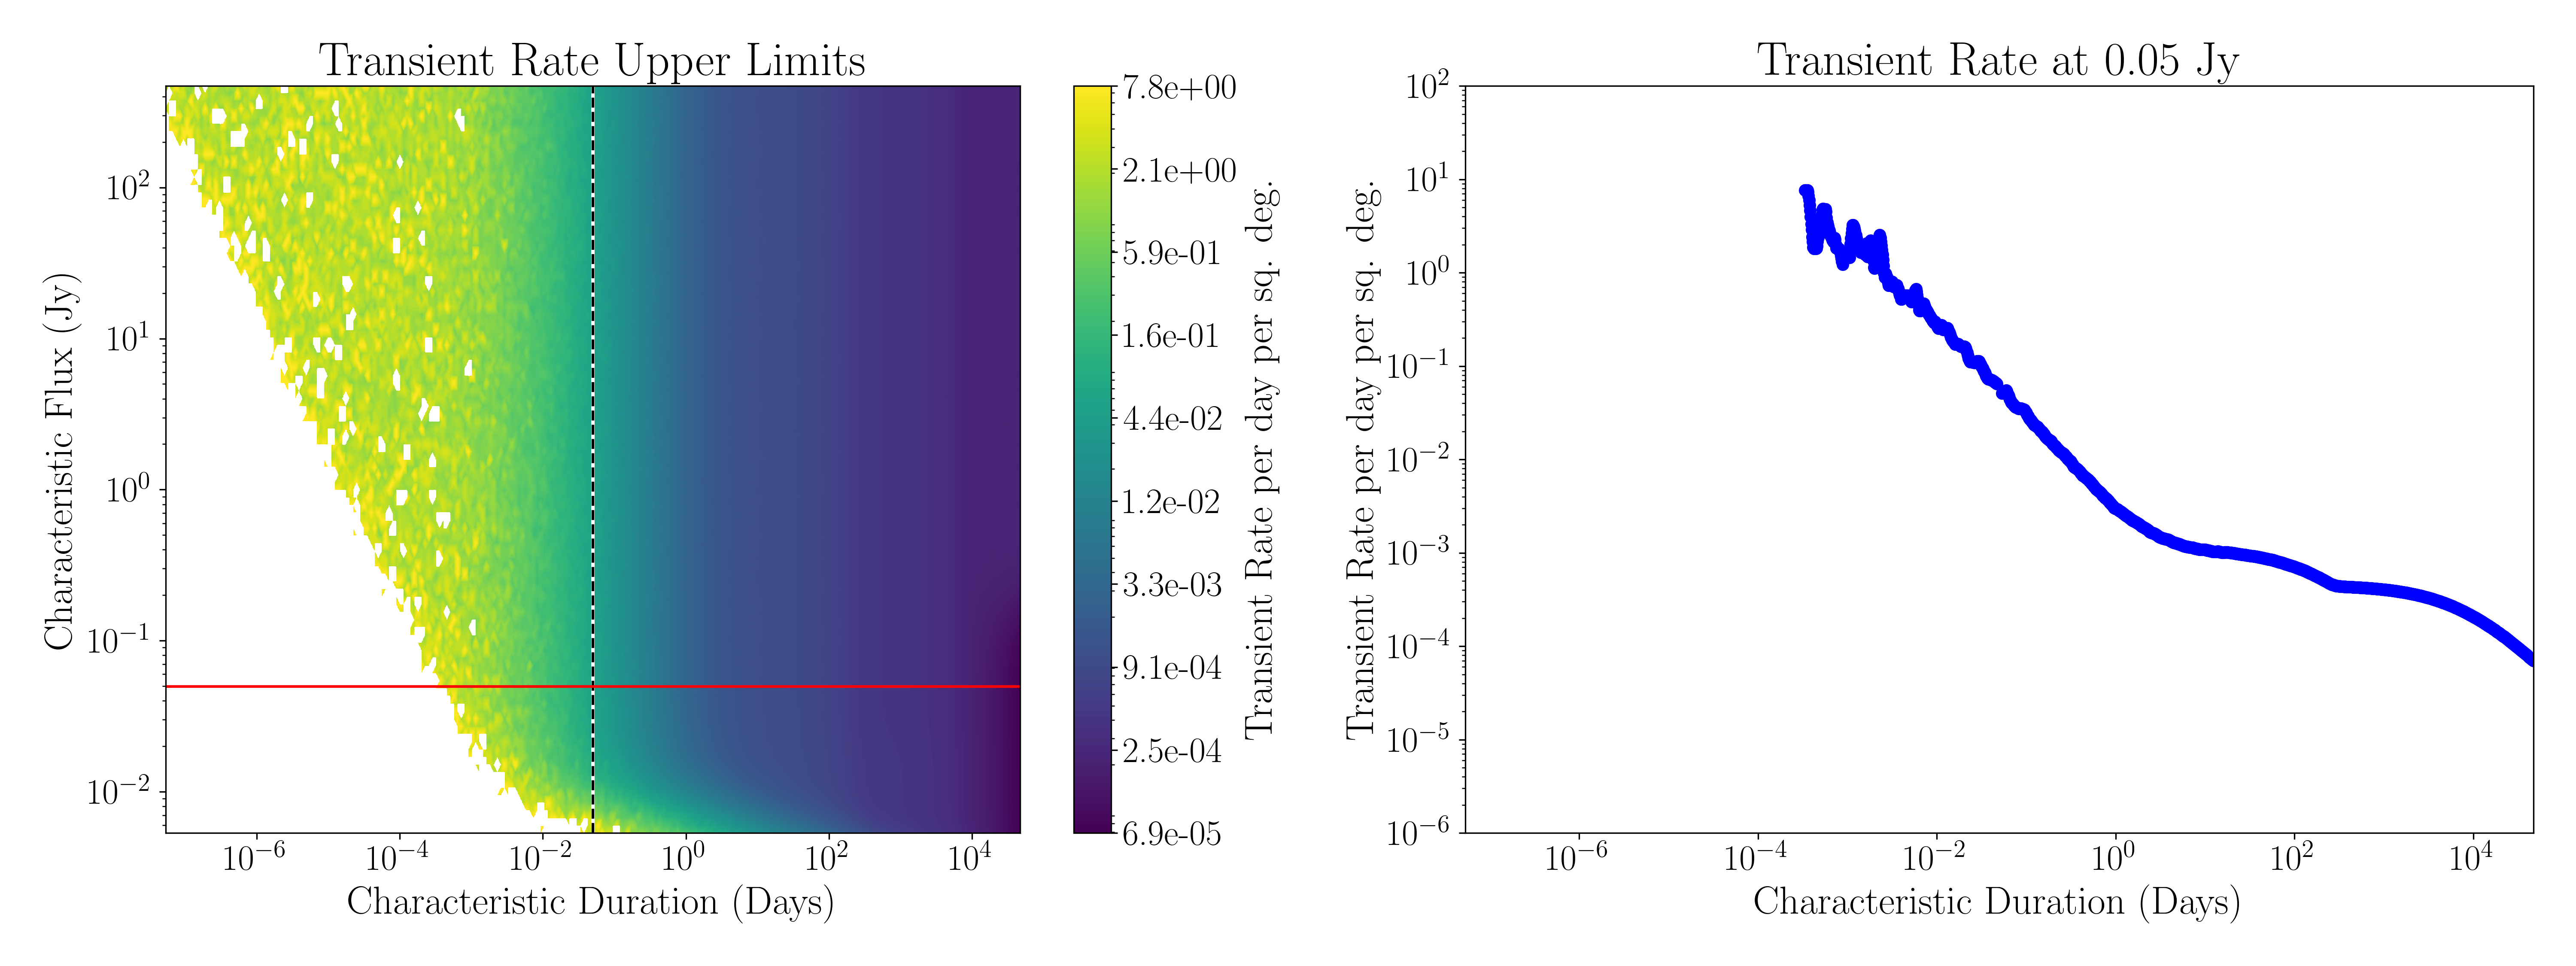
\includegraphics[width=\textwidth]{bowerandsauletal.png}
	\caption{Transient rate limits for a survey similar to~\citet{2011ApJ...728L..14B}. The vertical dashed line in the left panel marks where two different simulations were combined into a single plot; the horizontal red line marks 50 mJy. The panel on the right shows the transient rate as a function of duration at 50 mJy.}
	\label{fig:bowerandsaulall}
\end{figure}

\subsubsection{Comparing Limits on FRBs}
We examined the possibility of detecting an FRB in our survey. FRBs have timescales that are much shorter than the timescale of our observations, down to milliseconds. However, the flux of these sources is also quite high, exceeding Jansky levels. For this reason, it may be possible to detect an FRB in the 8 second images since the total fluence may be sufficient for it to be detected. Note that in this study we are limited to full bandwidth observations and may miss a burst that is relatively narrow-band. Future surveys could present opportunities to search for narrow-band transient events by splitting up the observations in frequency.
 For example \citet{2023MNRAS.518.3462A}, detected an FRB in two second images and would have been able to detect the brightest bursts in eight second images.  \citet{2021ApJS..257...59C} calculates the rate of FRBs based on CHIME observations to be $820\pm 60 (\text{stat.})_{-200}^{+220}(\text{sys.})$ per sky per day. If we convert this value to a transient rate per square degree we find: $1.99\times10^{-2}\pm0.15_{-0.49}^{+0.53}$. The fluence in conjunction with the integration time of the observations is what determines what is detectable in a survey. The minimum fluence that we can detect is approximately 10 Jy ms. The transient rate at this fluence is approximately $2.5\times10^{-2}$ transients per day per square degree.  If we follow the scaling outlined in~\citet{2021ApJS..257...59C}, we can use $\alpha=-1.4$, where $\alpha$ is the power-law index for the scaling of FRB-like sources above a certain fluence, to rescale the fluence we detect to compare it with CHIME. From this we find a modified upper limit of approximately $6.6\times10^{-2}$  possible FRB-like transients per day per square degree. 
 
 By comparison, the minimum fluence of a survey like~\citet{2011ApJ...728L..14B} is around 1 kJy ms. Our survey does not yet give limits on transient rates that would be below that of the CHIME FRB rates. In order to see the feasibility of discovering an FRB-like event in a survey like ours, we simulate the same 8-second timescale images in our survey but with the observation continuing for another two years with a similar set-up. The resulting transient rates can be seen in Figure~\ref{fig:doublerate}. From this figure we see that the upper limit on the transient rate would be around $10^{-1}$ transients per day per square degree at the same minimum fluence as before. Rescaling the fluence results in an upper limit of $2.64\times 10^{-1}$ possible FRB events per day per square degree. This means that with a doubling of the survey length, we still will not quite be able to place tighter limits on the FRB population. However, since this search is a commensal search and these limits are approaching the rates set by CHIME, it is worthwhile to continue to search for these short timescale transients in order to refine our understanding of them. 
\begin{figure}
	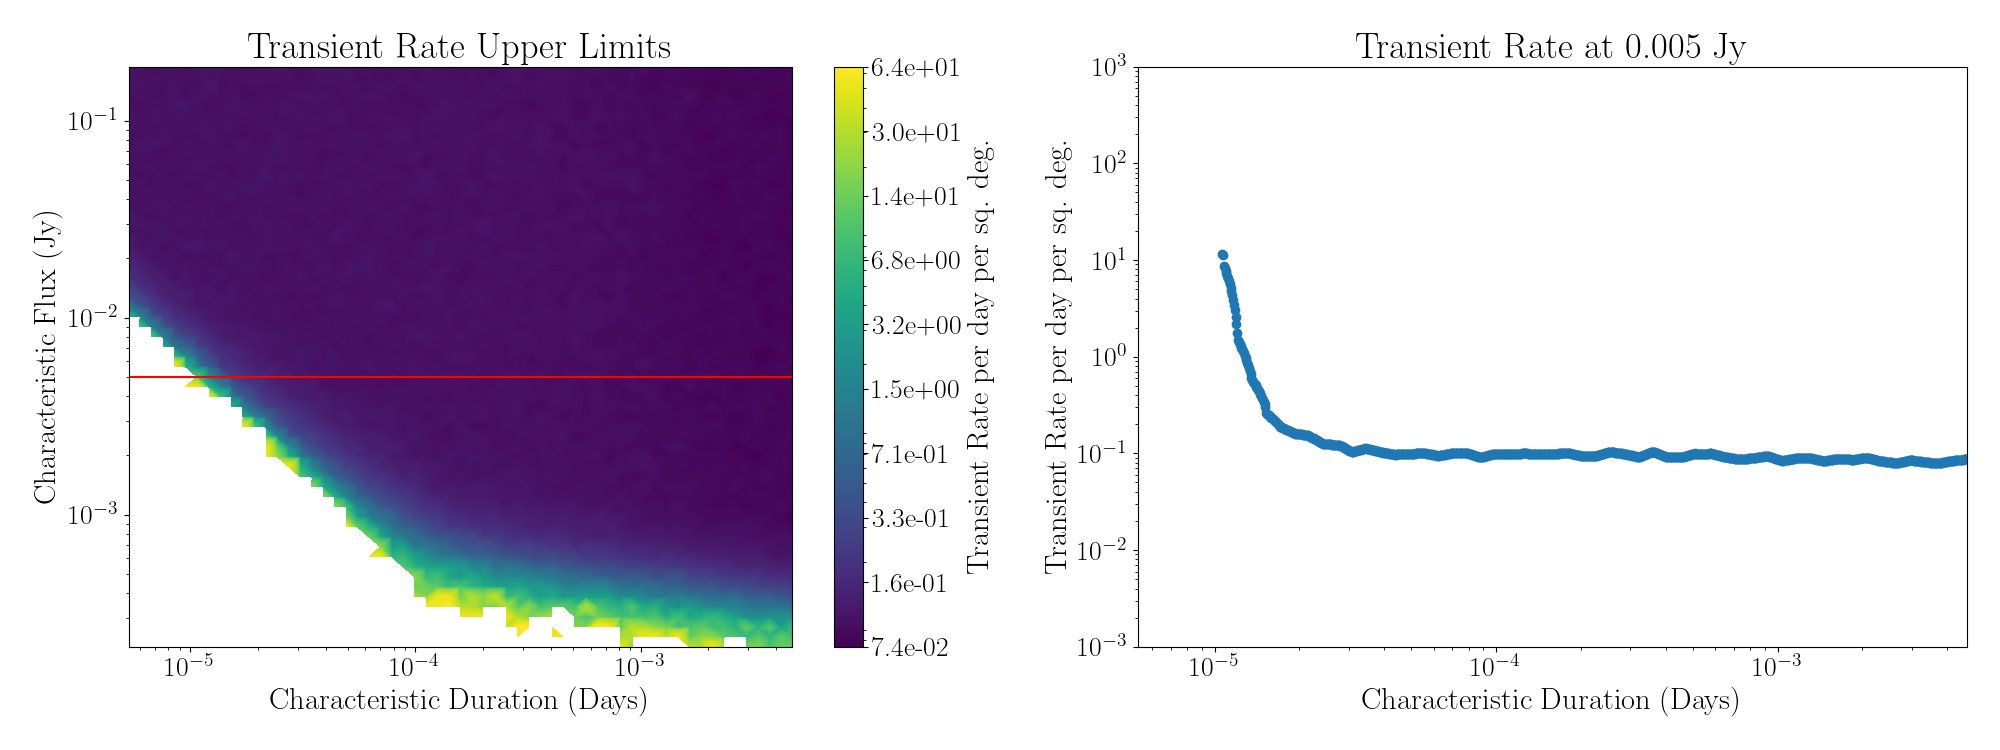
\includegraphics[width=\textwidth]{doublerealint.png}
	\caption{Transient rate upper limits, calculated using~\citet{2022ascl.soft04007C}, for a survey exactly double in duration of the 8-second timescale survey.}
	\label{fig:doublerate}
\end{figure}

\subsection{Conclusion}
We search deep MeerKAT observations of short gamma-ray burst fields for transients and variable sources, by making images with integration times of 4 hours, 15 minutes, and 8 seconds. This results in a transient survey that spans timescales from seconds to months. We search for transients in these images using the LOFAR Transients Pipeline~\citep{2015A&C....11...25S}. While we do not find any significant transients in the 8-second and 15-minute images, we find more than 120 variables in the long observations. Most of the variability can be explained by interstellar scintillation effects on the radio emission from active galactic nuclei. However, in a few cases the variability is likely intrinsic, because the observed modulation and variability timescales differ significantly from expectations and the variability observed in other sources in those fields. We also place new, accurate limits on the transient rate using transient simulations~\citep{2022ascl.soft04007C}. Our limits at the shortest timescales and lowest fluence levels are approaching the limits placed by time series searches at sub-second timescales such as those for FRBs with CHIME \citep{2021ApJS..257...59C}. Continued commensal searches, in conjunction with refining the techniques for transient searches that are described here, should continue to constrain transient rates calculated from image searches and approach the rates found for sources such as FRBs, thus providing a new method for studying transients on short timescales.

\subsection{Acknowledgments}
We would like to thank Geoff Bower for sharing information and data from \citet{2011ApJ...728L..14B}. 

The MeerKAT telescope is operated by the South African Radio Astronomy Observatory (SARAO), which is a facility of the National Research Foundation, an agency of the Department of Science and Innovation. We would like to thank the operators, SARAO staff and ThunderKAT Large Survey Project team.

We acknowledge use of the Inter-University Institute for Data Intensive Astronomy (IDIA) data intensive research cloud for data processing. IDIA is a South African university partnership involving the University of Cape Town, the University of Pretoria and the University of the Western Cape. We also acknowledge the computing resources provided on the High Performance Computing Cluster operated by Research Technology Services at the George Washington University.

This work was completed in part with resources provided by the High Performance Computing Cluster at The George Washington University, Information Technology, Research Technology Services.

The catalogs that were searched for multi-wavelength counterparts and included in Figure~\ref{fig:combinedfluxfluxplots} are~\citet{vizier:V/156,vizier:V/154,vizier:J/ApJS/249/18,vizier:J/ApJ/794/120,vizier:J/A+A/540/A106,vizier:II/371,vizier:II/358,vizier:II/349,2006AJ....131.1163S,vizier:II/367,vizier:II/319,vizier:II/246,vizier:B/denis,vizier:J/ApJS/225/1,vizier:II/363,vizier:II/328,vizier:II/311,1998AJ....115.1693C,vizier:VIII/92}.

%%%%%%%%%%%%%%%%%%%%%%%%%%%%%%%%%%%%%%%%%%%%%%%%%%
\section*{Data Availability}


Data is available upon request by email to schastain@gwu.edu.






% \begin{figure}
	% \includegraphics[width=\textwidth]{LEGACY/src713717lc4.png}
	% \caption{On the left is the light curve plotted with linear scaling. On the right, it is plotted on a log-log plot with time measured from the start of the GRB trigger that the image is targeting. }
	% \label{fig:src715717lc4.png}
	% \end{figure}
\newpage
\section{Commensal Transient Searches in SNe and GRB Fields}

With the establishment of new radio telescopes such as MeerKAT~\citep{2009IEEEP..97.1522J}, ASKAP~\citep{2008ExA....22..151J}, and LOFAR~\citep{2013A&A...556A...2V}, large areas of the sky are being imaged in a relatively short period of time. This leads to surveys such as the LOFAR Multi-frequency Snapshot Survey \citep[MSSS;][]{2016MNRAS.456.2321S}, the ASKAP Variables and Slow Transients Survey \citep[VAST;][]{2021PASA...38...54M}, and the Rapid ASKAP Continuum Survey \citep[RACS;][]{2020PASA...37...48M}. One transient was found in MSSS with a duration of 10 minutes, while the VAST and RACS surveys are ongoing and promise to find transients and variables in larger quantities due to their large fields of view and good sensitivity. In addition to these dedicated surveys, commensal transient searches in MeerKAT data have yielded results as well: the first MeerKAT transient was found in the same field as the black hole X-ray binary GX 339-4~\citep{2020MNRAS.491..560D}, along with several variable sources \citep{2022MNRAS.512.5037D}; and several variables were found in the same field as the black hole X-ray binary MAXI J1820+070 \citep{2022MNRAS.517.2894R}. In addition, \citep{commensal1} recently presented the results of commensal searches for transients on multiple timescales in eight short gamma-ray burst (GRB) fields. In this search, a large number of variables was found, of which 120 were variable due to interstellar scintillation and 2 showed possible intrinsic variability. All these sources were variable on time scales of days to months, and searches at shorter timescales, 15 minutes and 8 seconds, did not result in significant transient detections.

In the study presented here, we perform a commensal search in fields of supernovae (SNe) and short GRBs observed by MeerKAT. These fields have been observed for 4 to 5 hours at a time, which allows for transient searches between different epochs but also at shorter timescales. We follow the methodology of \citet{commensal1}, in particular the software and techniques established in that study, by making images with approximately 30-minute integration times. This allows us to probe the transient parameter space at timescales of hours, but also on timescales of days to years by comparing multiple observations of the same field.

In the Observations section, we describe the observations used in the survey and data processing strategies. In the Methods section, we describe the techniques and software used to find transient sources in the images. Then, in the Results section, we give an overview of the interesting sources that came out of our search. This is followed by the Discussion section, in which we discuss the possible counterparts and identification of the sources we find, along with the limits on the transient rate as a result of this survey. Finally, in the Conclusions we draw overall conclusions based on this study.

\subsection{Observations}
\label{sec:observations3}
Deep observations were taken of short GRB and SN fields. Each observation was around 4 to 5 hours in length, not including calibration overheads, and the entire set of observations is summarized in Tables~\ref{tab:allobs3} and~\ref{tab:allobs3cals}. During the observations, the pointing of the telescope cycled between the target for approximately 15 minutes and a complex gain calibrator for about 5 minutes. In addition, a bandpass and flux calibrator was observed for several minutes. Both of these calibrators are also listed for each observation in this table.
\newgeometry{margin=1.25in} % modify this if you need even more space
\begin{landscape}
\begin{deluxetable}{llrrr}
	\tablecolumns{5}
	\tablewidth{0pc}
	\tablecaption{All observations used in this study, indicating the observations' start and end times, phase center position, and time spent on the target. \label{tab:allobs3}}
	\tablehead{\colhead{Name} &  \colhead{Observation Time} &   \colhead{RA} &  \colhead{DEC} &    \colhead{Time On Target} \\ 
	\colhead{} &  \colhead{(UT)} &   \colhead{(deg)} &  \colhead{(deg)} &    \colhead{(hrs)}  \\}
	\startdata
  SN2019np & 2019-01-11 23:15:47.5 $-$ 2019-01-12 03:56:56.4 & 157.3415 &  29.5107 &                  3.22 \\
  SN2019np &  2019-03-10 19:50:15.6 $-$ 2019-03-11 00:13:8.9 & 157.3415 &  29.5107 &                  2.97 \\
 SN2019muj & 2019-08-09 00:09:48.9 $-$ 2019-08-09 05:08:41.4 &  36.5771 &  -9.8359 &                  4.11 \\
  SN2020ue & 2020-01-14 01:43:23.7 $-$ 2020-01-14 06:12:48.9 & 190.6949 &   2.6595 &                  3.60 \\
  SN2020ue & 2020-01-19 23:14:52.5 $-$ 2020-01-20 03:46:49.6 & 190.6949 &   2.6595 &                  3.61 \\
  SN2020ue & 2020-02-06 00:55:23.8 $-$ 2020-02-06 05:28:24.9 & 190.6949 &   2.6595 &                  3.62 \\
 SN2020hvf & 2020-04-24 15:44:50.4 $-$ 2020-04-24 21:22:13.9 & 170.3602 &   3.0147 &                  4.98 \\
 SN2020hvf &  2020-05-01 17:15:5.2 $-$ 2020-05-01 22:50:12.7 & 170.3602 &   3.0147 &                  4.97 \\
 SN2021smj & 2021-07-10 12:45:57.1 $-$ 2021-07-10 18:51:27.9 & 186.6940 &   8.8827 &                  4.95 \\
 SN2021smj & 2021-07-23 11:50:54.9 $-$ 2021-07-23 17:57:13.6 & 186.6940 &   8.8827 &                  4.95 \\
 SN2021qvv &   2021-08-09 11:07:9.8 $-$ 2021-08-09 15:48:2.6 & 187.0122 &   9.8056 &                  3.96 \\
 SN2021smj &  2021-09-05 08:41:42.0 $-$ 2021-09-05 14:48:8.7 & 186.6940 &   8.8827 &                  4.95 \\
 SN2022ffv &  2022-03-31 09:22:5.0 $-$ 2022-03-31 15:01:52.3 &  54.1238 & -35.2893 &                  4.97 \\
 SN2022ffv & 2022-04-01 09:29:45.1 $-$ 2022-04-01 17:21:37.1 &  54.1238 & -35.2893 &                  4.97 \\
 SN2022ffv &  2022-04-14 08:22:1.1 $-$ 2022-04-14 14:01:48.5 &  54.1238 & -35.2893 &                  4.98 \\
GRB220730A &  2022-08-01 18:36:8.7 $-$ 2022-08-01 22:40:46.5 & 225.0143 & -69.4959 &                  3.46 \\
GRB220730A & 2022-08-03 16:30:46.1 $-$ 2022-08-03 20:36:27.8 & 225.0143 & -69.4959 &                  3.47 \\
GRB220730A & 2022-08-10 15:15:52.6 $-$ 2022-08-10 19:22:14.4 & 225.0143 & -69.4959 &                  3.47 \\
GRB200522A &  2022-08-16 23:22:42.4 $-$ 2022-08-17 03:23:4.3 &   5.6820 &  -0.2832 &                  3.47 \\
GRB200907B & 2022-08-19 05:18:50.2 $-$ 2022-08-19 09:23:44.0 &  89.0290 &   6.9062 &                  3.47 \\
GRB210919A &   2022-08-20 05:17:2.6 $-$ 2022-08-20 09:19:8.5 &  80.2545 &   1.3115 &                  3.46 \\
GRB210726A &  2022-08-21 11:26:1.1 $-$ 2022-08-21 15:29:43.0 & 193.2909 &  19.1875 &                  3.46 \\
GRB200411A & 2022-08-22 02:16:28.7 $-$ 2022-08-22 06:03:30.9 &  47.6641 & -52.3176 &                  3.22 \\
GRB210323A & 2022-08-23 20:17:47.4 $-$ 2022-08-24 00:23:13.2 & 317.9461 &  25.3699 &                  3.47 \\
GRB200219A & 2022-08-24 00:47:39.5 $-$ 2022-08-24 04:52:25.3 & 342.6385 & -59.1196 &                  3.46 \\
GRB220730A & 2022-09-08 15:37:10.1 $-$ 2022-09-08 19:42:19.8 & 225.0143 & -69.4959 &                  3.46 \\
 SN2020eyj & 2022-05-07 16:10:32.8 $-$ 2022-05-07 21:05:17.3 & 167.9466 &  29.3893 &                  3.96 \\
 SN2020eyj &  2022-10-28 04:47:5.0 $-$ 2022-10-28 09:42:45.5 & 167.9466 &  29.3893 &                  3.97 \\
	\enddata
\end{deluxetable}
\end{landscape}
\begin{deluxetable}{lll}
	\tablecolumns{3}
	\tablewidth{0pc}
	\tablecaption{A table showing the calibrators used for each field in the study. \label{tab:allobs3cals}}
	\tablehead{\colhead{Name}  \colhead{Bandpass} & \colhead{Complex Gain} }
	\startdata
    SN2019np  &J1331+3030 &   J1120+1420 \\
  SN2019muj  &J0408-6545 &   J0240-2309 \\
   SN2020ue  &J1939-6342 &   J1256-0547 \\
  SN2020hvf  &J0408-6545 &   J1058+0133 \\
  SN2021smj  &J0408-6545 &   J1150-0023 \\
  SN2022ffv  &J0408-6545 &   J0440-4333 \\
 GRB220730A  &J1939-6342 &   J1619-8418 \\
 GRB200522A  &J1939-6342 &   J0022+0014 \\
 GRB200907B  &J0408-6545 &   J0521+1638 \\
 GRB210919A  &J0408-6545 &   J0503+0203 \\
 GRB210726A  &J1331+3030 &   J1330+2509 \\
 GRB200411A  &J0408-6545 &   J0210-5101 \\
 GRB210323A  &J1939-6342 &   J2236+2828 \\
 GRB200219A  &J0408-6545 &   J2329-4730 \\
 GRB220730A  &J1939-6342 &   J1619-8418 \\
  SN2020eyj  &J1120+1420 &   J0408-6545 \\
 	\enddata
\end{deluxetable}

\restoregeometry
 \doublespacing
Almost all observations were calibrated using version 2.0 of the ProcessMeerKAT pipeline, with the exception of the GRB~220730A observations that were processed using version 1.1 of the pipeline~\citep[{\sc ProcessMeerKAT};][]{pminprep}. As part of the calibration process, parts of the spectrum known to be heavily contaminated with radio frequency interference (RFI) were flagged, resulting in a bandwidth of approximately 800 MHz centered at 1.3~GHz. Calibration was performed in parallel over 9 spectral windows (11 for ProcessMeerKAT 1.1). Common Astronomy Software Applications~\citep[{\sc CASA;}][]{2022arXiv221002276T} tools were used to perform complex gain and flux calibration, along with flagging for RFI, using the tasks tfcrop and rflag. After two rounds of calibration and flagging, the spectral windows were recombined into a single measurement set for imaging.

Imaging was performed using tclean, with parameters to account for non-coplanar baselines. The w-project gridder was used with 128 planes, the gain was set to 0.08, and multi-term multi-frequency synthesis was used with 2 Taylor series terms and scales of 0, 5, and 15. The imaging process started with a shallow image, using a threshold of 1 mJy. This image was used to create a model for phase self-calibration. Additional RFI flagging was also performed using rflag. After self-calibration, images with an integration time of approximately 30 minutes were created by combining adjacent 15 minute scans into a single image. Finally, primary beam correction was performed using the katbeam library \citep{2022AJ....163..135D}. The average noise and the number of images is summarized in Table~\ref{tab:obstimescales}. 


\begin{deluxetable}{lll}
	\tablecolumns{3}
	\tablewidth{0pc}
	\tablecaption{Summary of number of images of each field and the average noise. \label{tab:obstimescales3}}
	\tablehead{ \colhead{Target} & \colhead{\# of images} & \colhead{Avg. RMS Noise} \\
		\colhead{} & \colhead{} & \colhead{($\mu$Jy)}}
	\startdata
	SN2019np & 12 & 31\\
	SN2019muj & 21 & 31\\
	SN2020ue & 33 & 37\\
	SN2020hvf & 10 & 20\\
	SN2021smj & 30 & 44\\
	SN2021qvv & 8 & 77\\
	SN2022ffv & 17 & 38\\
	GRB220730A & 28 & 23\\
	GRB200522A & 7 & 140\\
	GRB200907B & 7 & 47\\
	GRB210919A & 7 & 96\\
	GRB210726A & 7 & 33\\
	GRB200411A & 6 & 19\\
	GRB210323A & 7 & 27\\
	GRB200219A & 7 & 21\\
	SN2020eyj & 16 & 36\\
	\enddata
\end{deluxetable}

\subsection{Methods}
\label{sec:methods3}

We used the LOFAR Transients Pipeline~\citep[{\sc TraP};][]{2015A&C....11...25S} for source finding, source association, and image quality control. TraP is also designed to calculate variability metrics based on source light curves, but we chose to do these calculations separately in order to account for a 10\% systematic error. Quality control is taken care of in TraP through multiple checks. The rms noise is measured in the inner part of the image by removing bright pixels. The measured noise in the image is compared to global allowed minimum and maximum values and put into a running histogram. After the first 100 images, if the noise is greater than 3$\sigma$ from the mean, it is rejected. This resulted in the rejection of six images. There are other reasons that an image could have been rejected, such as beam shape, for which we relaxed the ellipticity requirements to a factor of 10, and with that, these six images were the only rejected ones. 

Before determining variability, we only selected sources that were within 0.8 degrees of the center of the field. Given the fall-off of sensitivity and complex shape of the beam, this restriction prevents effects on the flux of our sources in ways that are difficult to model accurately. We calculated the variability measures V and $\eta$ for every source found by TraP, incorporating a 10\% systematic error into the calculations of $\eta$. We considered sources with an $\eta > 2$ to be a candidate variable. This value was chosen in our first study \citep{commensal1} by examining a large number of sources and examining the variability in histograms.  We also determined a signal-to-noise detection threshold in the same way as \citet{2022MNRAS.517.2894R} and \citet{commensal1}. We took a sample of 50\% of the pixels that were included in the transient search and determined the threshold at which less than 1 false transient detection would occur by assuming the pixels follow a Gaussian distribution. Using this method, we determined a threshold of approximately 5.4 times the rms noise in the image. This threshold is only a rough approximation since the pixels do not follow a Gaussian distribution; see Figure~\ref{fig:pixels} and the discussion in \citet{2022MNRAS.517.2894R}. 

In order to reduce the number of sidelobes flagged as potential transients, we rejected all but the brightest source in a circular region of 5 beam widths around every source (measured by the beam's major axis), following \citet{commensal1}. Some sidelobes still remained after this step, and we could have made this radius larger to attempt to remove more artifacts, but we did not want to risk losing any more potential candidates, so we removed these sidelobe sources in later steps by visual determination.
\begin{figure}
	% 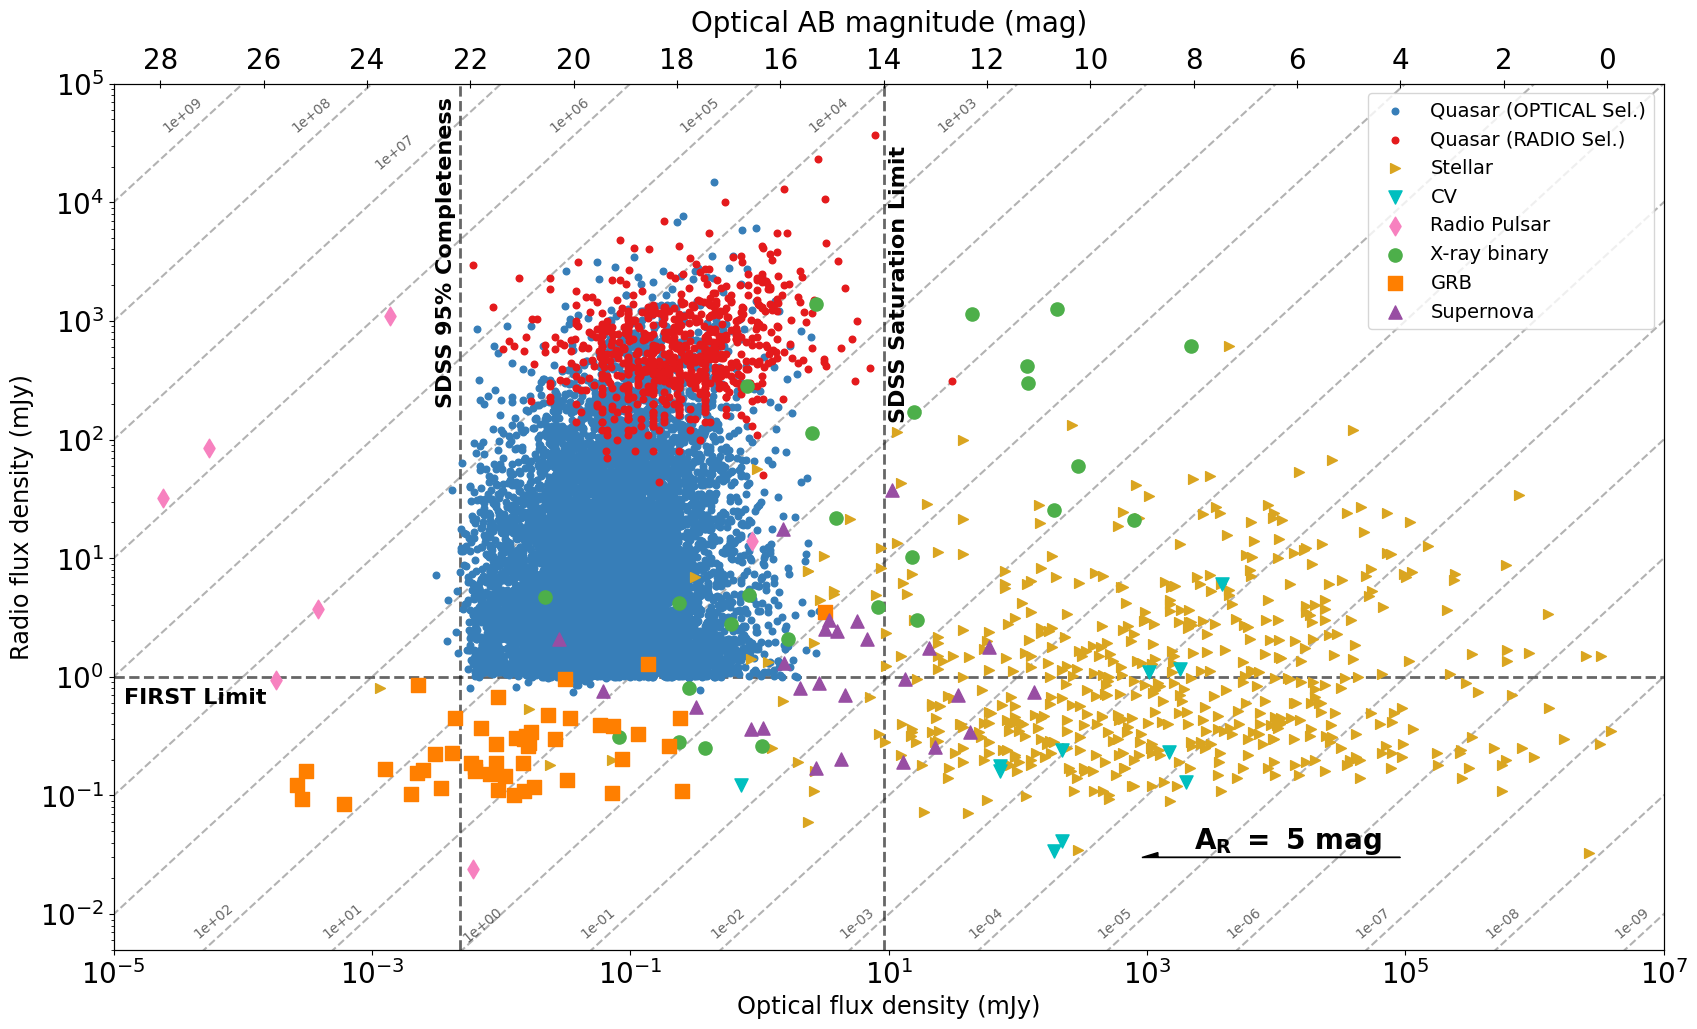
\includegraphics[width=0.9\textwidth]{ro_figure_1.png}
	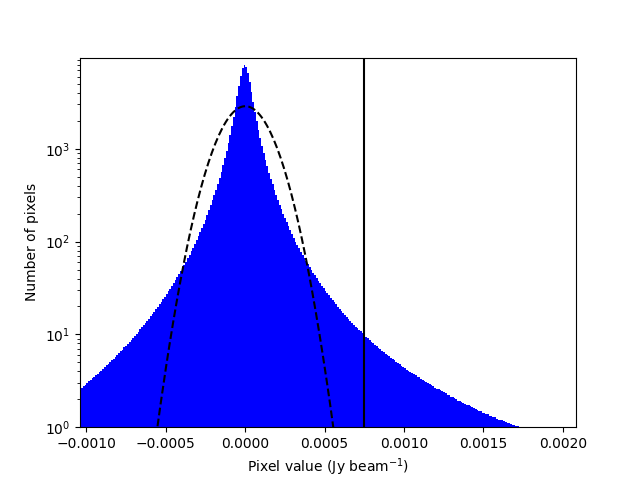
\includegraphics[width=\columnwidth]{pixels.png}
	\caption{A plot of the sample of pixels used for determining the detection threshold along with the fitted Gaussian.}
	\label{fig:pixels}
\end{figure}
\subsection{Results}
\label{sec:results3}

After we performed the aforementioned steps to find transients, and then systematically reduced the number of spurious sources, we were left with 874 sources that had an $\eta$ value greater than 2 or with a detection in only a single image. We made animations of these sources\footnote{Code available at https://github.com/dentalfloss1/sharedscripts as FindOutliers.py} to further categorize them. After visual examination, 289 sources were identified as sidelobes of brighter sources, 477 sources needed further examination with higher contrast, 57 sources were due to noise patterns, 24 sources appeared to be astrophysical sources, and 28 sources failed to make a proper animation likely due to only being detected in a single image. Next, a forced fit was done of the 477 sources that needed higher contrast, the 28 sources that did not make an animation properly, and the 24 sources that appeared to be astrophysical sources. After this step, only 52 sources remained with an $\eta$ value above two. Each of the 52 sources were examined carefully, and sources that appeared to have variability due to issues with the image, such as the beam shape causing two sources to merge into one, or an extremely bright source causing issues across the image, were rejected, leaving 14 sources. 

Out of these 14 sources, 11 showed variability from observation to observation; see, for example, Figure~\ref{fig:src1290071multi}. In three of these 11 sources, the 30-minute images showed also variability within the $4-5$~hour observation, which was likely due to a bright source in the field. For these sources, we re-ran TraP on the full observations, measuring the corrected $\eta$ value for each of the three sources. After this step, the corrected $\eta$ value for one of the sources was less than two and this source was removed from consideration. Therefore, our final count of variables in this data set is 13.




\subsection{Discussion}
\label{sec:discussion3}
\subsubsection{Sources with Radio Counterparts}

Six of the variables we found in our study have radio counterparts in various catalogs. These sources together with their counterpart measurements are shown in Table~\ref{tab:radiocounterparts}, along with the forced flux measurement at the location of a seventh source (1278651; see below). In addition, the light curves for these sources are shown in Figures~\ref{fig:src1290071multi}-\ref{fig:src1279472multi}. 

Our measurements from MeerKAT at 1.3~GHz agree fairly well with the catalog measurements at other times. There is one notably bright source, source 1267266, which showed variability between the NVSS and FIRST surveys. The integrated flux was 10 mJy in NVSS and 7.2 mJy in FIRST. In Figure~\ref{fig:src1267266multi}, we see this same range of variability in the MeerKAT data as well. 

Source 1278651 had no counterparts in other radio surveys. The non-detection in VLASS is particularly notable, since the limits given in Table~\ref{tab:radiocounterparts} are around a factor of three lower than our measurements at 1.3~GHz (see also Figure~\ref{fig:src1278651multi}). This could be due to variability in the time between observations; a steep spectral index of the source between 1.3 and 3~GHz; or, given that this source is around 0.77 degrees from the center of the image, issues with the primary beam correction resulting in the flux being overcorrected.

\newgeometry{margin=1.25in} % modify this if you need even more space
\begin{landscape}
\begin{deluxetable}{llllllll}
	\tablecolumns{8}
	\tablewidth{0pc}
	\tablecaption{A table showing radio catalog counterparts for variable sources in our survey. When indicated, source measurements were made by using the Python Source Extractor~\citep[{\sc PYSE};][]{2018ascl.soft05026S} on image cutouts acquired from CIRADA. VLASS data is from~\citet{2021ApJS..255...30G}, NVSS data is from~\citet{1998AJ....115.1693C}, FIRST data is from~\citet{2015ApJ...801...26H}, and RACS data is from~\citet{RACS1} and~\citet{RACS2}. Source 1278651 is a non-detection and a forced fit using PYSE is shown. \label{tab:radiocounterparts}}  
	\tablehead{		\colhead{Source} &       \colhead{RA }&     \colhead{ DEC} &    \colhead{$F_{int}$}  &    \colhead{$F_{pk}$}&  \colhead{ Freq.} &               \colhead{ Date} &       \colhead{Comparison Source} \\
	\colhead{}	&    \colhead{  }  &   \colhead{ }   &  \colhead{ (mJy)}  &    \colhead{(mJy)} & \colhead{  (GHz)} &  \colhead{ } &        \colhead{}        \\      }
	\startdata
       1252675 & 157.3791 &  29.8533 &       $2.3 \pm 0.5$ & $1.4 \pm 0.2$ & 2.7 & 2019-04-22 23:38:59 &        VLASS \\
       1260388 & 191.0687 &   2.3340 &       $1.6 \pm 0.3$ & $1.3 \pm 0.1$ & 2.7 &  2019-04-21 08:11:40 &        VLASS \\
       1260578 & 190.8379 &   2.4131 &       $1.5 \pm 0.3$ & $1.2 \pm 0.1$ & 2.7 &  2019-04-21 08:11:58 &        VLASS \\
       1267266 & 170.4347 &   2.8388 &        $10.0 \pm 0.5$ & ...        & 1.4 &  1995-02-27  &         NVSS \\
       1267266 & 170.4347 &   2.8388 &        $7.2$         & $7.2$       & 1.4 &  1998-07-01  &        FIRST \\
       1267266 & 170.4347 &   2.8388 &        $6.1 \pm 0.2$ & $6.1 \pm 0.2 $& 2.7 & 2018-01-12 11:12:44 &        VLASS \\
       1267266 & 170.4347 &   2.8388 &        $8.8 \pm 1.4$ & $7.2 \pm 0.4 $& 0.89 & 2020-05-01 12:50:35 &         RACS\\
       1279472 &  53.7036 & -35.6255 &        $1.2 \pm 0.3$ & $1.1 \pm 0.2$ & 2.7 &  2020-10-29 07:01:24 & VLASS (PySE) \\
       1279472 &  53.7036 & -35.6255 &        $1.2 \pm 0.3$ & $1.1 \pm 0.2$ & 2.7 &  2020-10-29 07:01:50 & VLASS (PySE) \\
       1290071 & 224.7278 & -69.5997 &        $1.2 \pm 0.3$ & $1.2\pm 0.2$ & 0.89 & 2019-05-07 12:41:05 &  RACS (PySE)\\
       1290071 & 224.7278 & -69.5997 &        $1.2 \pm 0.3$ & $1.2 \pm 0.2$& 0.89 & 2019-05-07 13:27:32 &  RACS (PySE) \\
       1290071 & 224.7278 & -69.5997 &        $1.2 \pm 0.3$ & $1.2 \pm 0.2$ & 0.89 & 2020-05-02 15:48:10 &  RACS (PySE) \\
       1290071 & 224.7278 & -69.5997 &        $1.2 \pm 0.3$ & $1.2 \pm 0.2$ & 0.89 & 2020-06-19 13:35:51 &  RACS (PySE) \\
       \hline
       1278651 & 54.8335 & -35.8063 &        $0.74 \pm 0.71$ & $0.5 \pm 0.3$ & 0.89 & 2019-04-27 09:17:12 &  RACS (PySE) \\
       1278651 & 54.8335 & -35.8063 &        $0.72 \pm 0.7$ & $0.5 \pm 0.3$ & 0.89 & 2019-04-28 07:38:54 &  RACS (PySE) \\
       1278651 & 54.8335 & -35.8063 &        $0.79 \pm 0.71$ & $0.6 \pm 0.3$ & 0.89 & 2019-04-28 08:56:12  &  RACS (PySE) \\
       1278651 & 54.8335 & -35.8063 &       $0.34 \pm 0.27$ & $0.3 \pm 0.1$ & 2.7 & 2020-10-29 07:01:24 &  VLASS (PySE) \\
	\enddata
\end{deluxetable}

	%put your table here

\end{landscape}
\restoregeometry
 \doublespacing

\subsubsection{Other Multi-wavelength Data and Classification}
In addition to the aforementioned radio data, all seven sources have optical and near-infrared detections. In Figure~\ref{fig:radoptplot}, we show these counterparts on a scatter plot with the radio peak measurements, plotting the near-infrared K filter instead of the optical R filter, to account for possible dust extinction effects in the optical. The clustering of sources in the figure suggests that these sources are possibly active galactic nuclei (AGN). These sources are not likely to be GRBs due to the variability timescales and lack of the characteristic power-law light curves. A total of eight sources, including all seven of the previously mentioned sources in Table~\ref{tab:radiocounterparts}, are extragalactic, having redshifts in the DESI Legacy Imaging Survey~\citep{10.1093...mnras...stac608}. 

\begin{figure}
	% 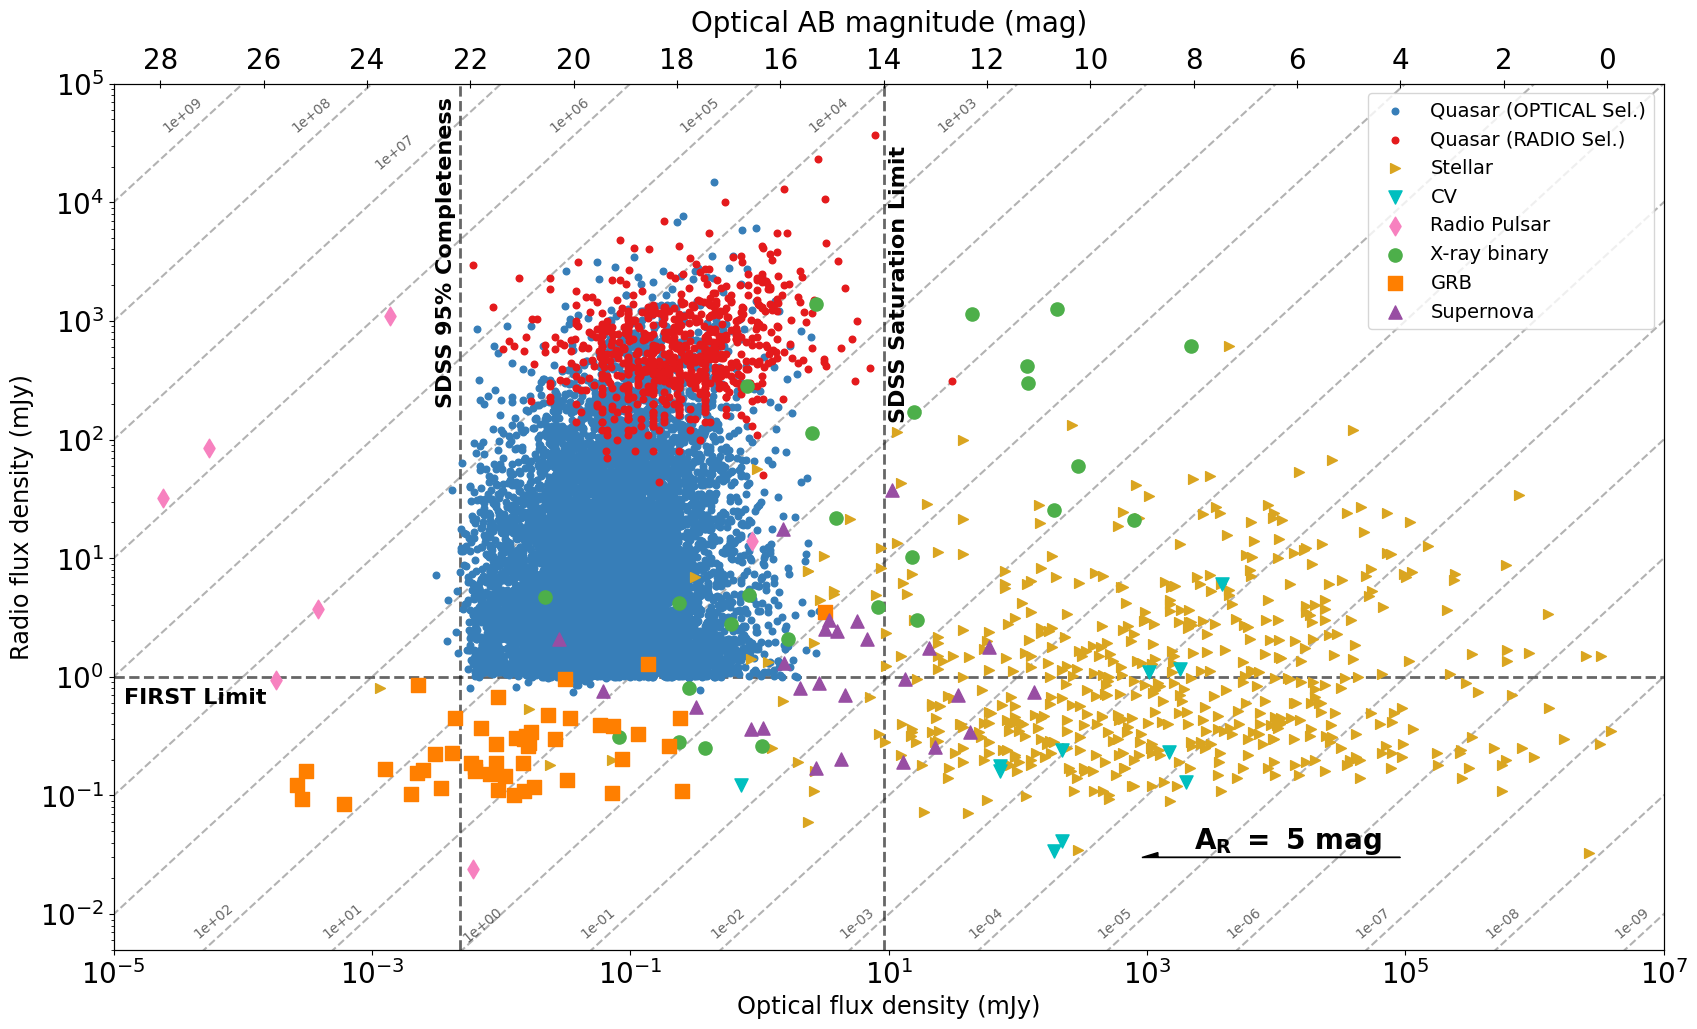
\includegraphics[width=0.9\textwidth]{ro_figure_1.png}
	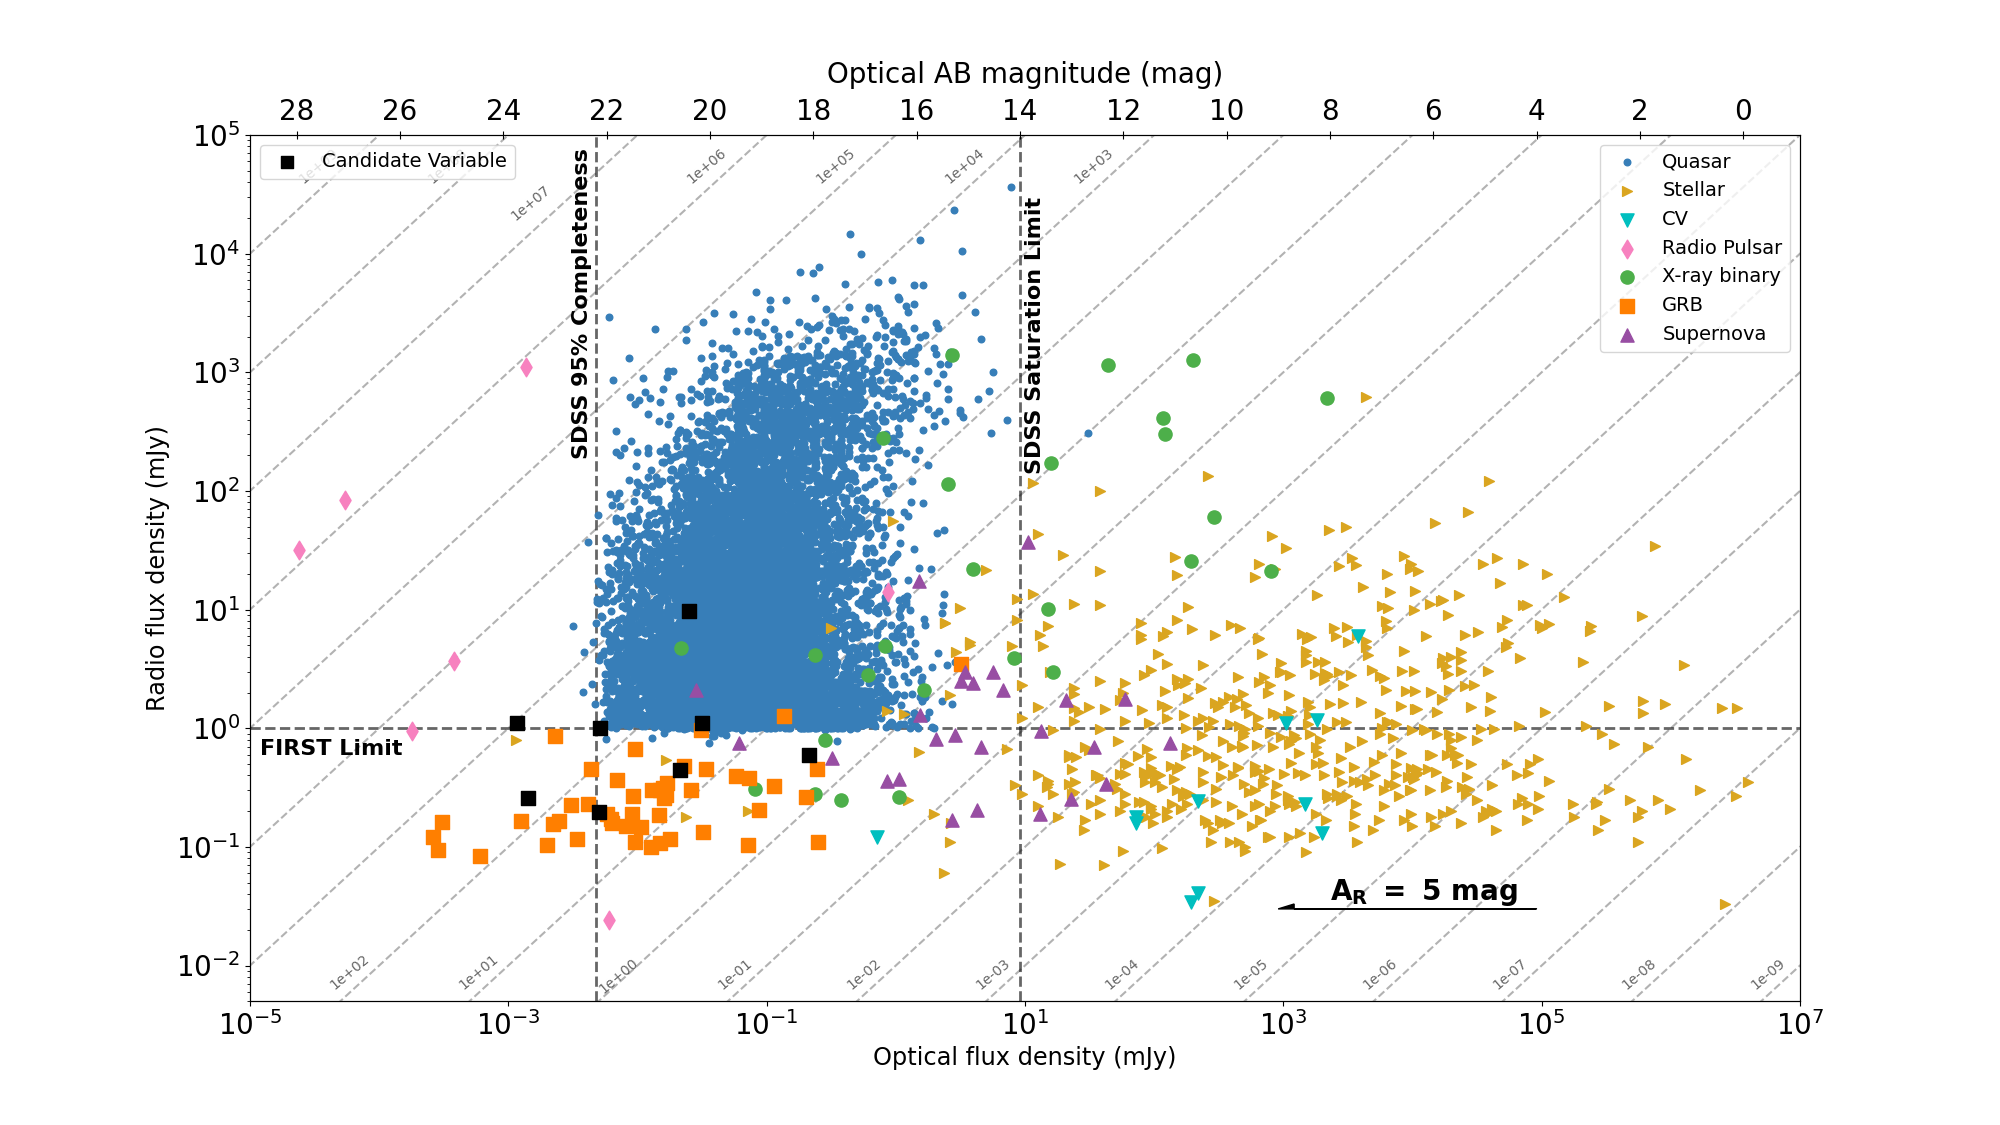
\includegraphics[width=\textwidth]{myradoptvars.png}
	\caption{A plot from~\citet{2018MNRAS.479.2481S} showing radio vs optical flux density for a variety of variable sources. Overplotted in black squares are the variable sources from our survey.}
	\label{fig:radoptplot}
\end{figure}

Source 1278651 has conflicting multi-wavelength catalog data: the Gaia early data release 3 catalog \citep{2021AJ....161..147B} shows a star approximately 1.3~kpc away within 1 arcsecond of the source, however, the parallax measurement of this source is of only about 2$\sigma$ significance. There is also a faint X-ray source at this location: \citet{2011ApJS..192...10L} detect a source with Chandra, reporting a distance of 12 Mpc, which is also present in the second Chandra Source Catalog~\citep{2010ApJS..189...37E}. These X-ray measurements hint at this source being an AGN.


\subsubsection{Interstellar Scintillation}

Interstellar scintillation is a common cause of variability in the radio sky. On the timescales and observing frequency probed here, refractive scintillation is the most dominant type of scintillation. It is caused by inhomogeneities in the ionized component of the interstellar medium. \citet{1998MNRAS.294..307W} provides an overview of interstellar scintillation with examples of its effects. For this survey, we use~\citet{2019arXiv190708395H} to compute expected values of refractive scintillation at the pointing center of each field. A summary of the resulting scintillation parameters are shown in Table~\ref{tab:scinttab}. Quite a few of these fields have very large modulation indices. These indices represent the fractional variation in flux, which we can use to compare to V, the variability metric calculated for each source. All of the sources we consider variable are shown in Table~\ref{tab:sourcevar}, with the variability statistics and an estimated upper limit on the timescale of variation estimated by visual inspection of the light curves. 


\begin{deluxetable}{lrrrrr}
	\tablecolumns{6}
	\tablewidth{0pc}
	\tablecaption{Scintillation properties at the center of each field calculated using~\citet{2019arXiv190708395H}. \label{tab:scinttab}}
	\tablehead{\colhead{Target} &     \colhead{  RA } &     \colhead{ Dec }&  \colhead{  m } &  \colhead{timescale} &  \colhead{ $\nu_0$} \\
	\colhead{}	&    \colhead{(deg)}    &   \colhead{(deg)}    &  \colhead{}     &  \colhead{(days)} &  \colhead{(GHz)}  }
	\startdata
 SN2019muj &  36.5771 &  -9.8359 & $0.69\pm   0.09$   &  $ 2.0 \pm         0.8$ &  2.5 \\
  SN2020ue & 190.6949 &   2.6595 & $0.53\pm   0.03$   &  $ 4.4 \pm         0.6$ &  3.9 \\
 SN2020hvf & 170.3602 &   3.0147 & $0.66\pm   0.07$   &  $ 2.3 \pm         0.8$ &  2.6 \\
 SN2021smj & 186.6940 &   8.8827 & $0.72\pm   0.11$   &  $ 1.7 \pm         0.8$ &  2.3 \\
 SN2021qvv & 187.0122 &   9.8056 & $0.71\pm   0.10$   &  $ 1.8 \pm         0.7$ &  2.3 \\
 SN2022ffv &  54.1238 & -35.2893 & $0.56\pm   0.13$   &  $ 3.9 \pm         2.7$ &  3.6 \\
 SN2020eyj & 167.9466 &  29.3893 & $0.65\pm   0.07$   &  $ 2.3 \pm         0.7$ &  2.7 \\
GRB220730A & 225.0143 & -69.4959 & $0.29\pm   0.01$   &  $64.1 \pm         9.5$ & 11.5 \\
GRB200522A &   5.6820 &  -0.2832 & $0.73\pm   0.12$   &  $ 1.7 \pm         0.8$ &  2.2 \\
GRB200907B &  89.0290 &   6.9062 & $0.30\pm   0.01$   &  $59.9 \pm         4.9$ & 10.9 \\
GRB210919A &  80.2545 &   1.3115 & $0.26\pm   0.01$   &  $64.5 \pm         4.2$ & 14.2 \\
GRB210726A & 193.2909 &  19.1875 & $0.66\pm   0.07$   &  $ 2.2 \pm         0.6$ &  2.7 \\
GRB200411A &  47.6641 & -52.3176 & $0.91\pm   2.20$   &  $ 0.9 \pm         6.7$ &  1.5 \\
GRB210323A & 317.9461 &  25.3699 & $0.37\pm   0.01$   &  $24.5 \pm         2.4$ &  7.5 \\
GRB200219A & 342.6385 & -59.1196 & $0.74\pm   0.65$   &  $ 1.7 \pm         4.6$ &  2.2 \\
  SN2019np & 157.3415 &  29.5107 & $0.66\pm   0.07$   &  $ 2.4 \pm         0.8$ &  2.7 \\
	\enddata
\end{deluxetable}


\begin{deluxetable}{lllllll}
\tablecolumns{7}
\tablewidth{0pc}
\tablecaption{This table shows all of the sources that are considered variable along with the variability statistics and the estimated timescale of variability. \label{tab:sourcevar}}
\tablehead{\colhead{Source} & \colhead{Field} & \colhead{RA} &   \colhead{Dec} &  \colhead{$\eta$} &    \colhead{V} &  \colhead{Timescale} \\
\colhead{}	& \colhead{} &\colhead{(deg)}      &  \colhead{(deg)}  \colhead{}   &  \colhead{} & \colhead{}    &  \colhead{(days)} \\ }
\startdata
1252675 & SN2019np & 157.3791 &  29.8533 & 6.03 & 0.12 &    $  <58$ \\
1252803 & SN2019np & 157.2391 &  29.9353 & 4.92 & 0.40 &    $  <58$ \\
1260388 & SN2020ue & 191.0687 &   2.3340 & 3.70 & 0.28 &    $  <17$ \\
1260578 & SN2020ue & 190.8379 &   2.4131 & 2.53 & 0.21 &    $  <17$ \\
1266989 & SN2020hvf & 170.5800 &   2.8567 & 2.98 & 0.21 &    $   <7$ \\
1267266 & SN2020hvf & 170.4347 &   2.8388 & 3.19 & 0.18 &    $   <7$ \\
1277302 & SN2020hvf & 170.4211 &   3.3767 & 8.53 & 0.44 &    $   <7$ \\
1278651 & SN2022ffv & 54.8335 & -35.8063 & 3.56 & 0.23 &    $  <13$ \\
1279472 &  SN2022ffv & 53.7036 & -35.6255 & 2.54 & 0.19 &    $   <0.8$ \\
1290071 & GRB220730A & 224.7278 & -59.5997 & 3.12 & 0.23 &    $  <29$ \\
1305970 & GRB200411A &  48.3284 & -52.7501 & 3.66 & 0.58 &    $   <0.02$ \\
1308228 & GRB200411A &  48.6663 & -52.4636 & 3.66 & 0.67 &    $   <0.02$ \\
1318936 & GRB200219A & 341.5495 & -59.0375 & 2.06 & 0.13 &    $   <0.06$ \\
	\enddata
\end{deluxetable}

Comparing Tables \ref{tab:sourcevar} and~\ref{tab:scinttab} shows that all but one source can be considered consistent with refractive scintillation. The upper limit on the timescale of variation in source 1290071 is about half of the expected scintillation timescale with the variability parameter, V, being close to the modulation index, m. It could be that the assumed distance to the scattering screen used in the calculation of the scintillation characteristics is much less, perhaps half of the assumed 1.5~kpc. This change would result in the timescale matching the estimated upper limit of the variability timescale, with the modulation index being consistent as well. However, in Table~\ref{tab:radiocounterparts} we see that the radio measurements at 890 MHz of the RACS counterpart are remarkably stable, even between the observations separated by about a year. It is not possible to rule out scintillation for this source, but of all the sources in this survey, this source is the most likely to be showing intrinsic variability. 

Source 1278651 has non-detections in RACS and VLASS. We can see from Table~\ref{tab:scinttab} that the modulation index for this source is quite high and the scintillation timescale is relatively short. Therefore these non-detections can be explained by refractive scintillation. 

% \subsection{J1456-6843: A Diffractively Scintillating Pulsar}
% Before later restricting the search radius to sources that were within 0.8 degrees from the center of the field, we were searching out to 1 degree from the center. During this search we found a particularly interesting source whose light curve is shown in Figure~\ref{fig:src1290472multi.png}. This source shows variability on multiple timescales with the present analysis showing definite variability on the timescale of hours to days. The variability timescale is much too short to be refractive scintillation. After searching for catalog matches, the source was found to coincide within one arcsecond of pulsar J1456-6843 according to the ATNF pulsar catalog~\citep{2005AJ....129.1993M}. \citet{2021MNRAS.501.4490K} include this source in their study of pulsar flux density variability and, using the dispersion measure, determine that this source shows diffractive scintillation. 



\subsubsection{Upper Limits on the Transient Rate}
Using the survey parameters along with the non-detection of any transients, we can place limits on the transient rate using the simulations code presented in \citet{2022ascl.soft04007C}. Figure~\ref{fig:transientrate} shows the upper limit on transient rates calculated for this survey. This was done by simulating transients, calculating transient rates for each field in the survey, and taking an average over the transient rates weighted by the survey duration of each field and field of view. Our strictest limits show an upper limit of $10^{-4}$ transients per day per square degree for transients with a duration of about 200 days and flux of 5 mJy. Compared to the limits we found in~\citet{commensal1}, this limit is approximately a factor of two lower at a similar transient duration. This may be due to this survey having a larger number of hours on target, 113 versus 100, combined with having higher quality images on average.

\begin{figure}
	% 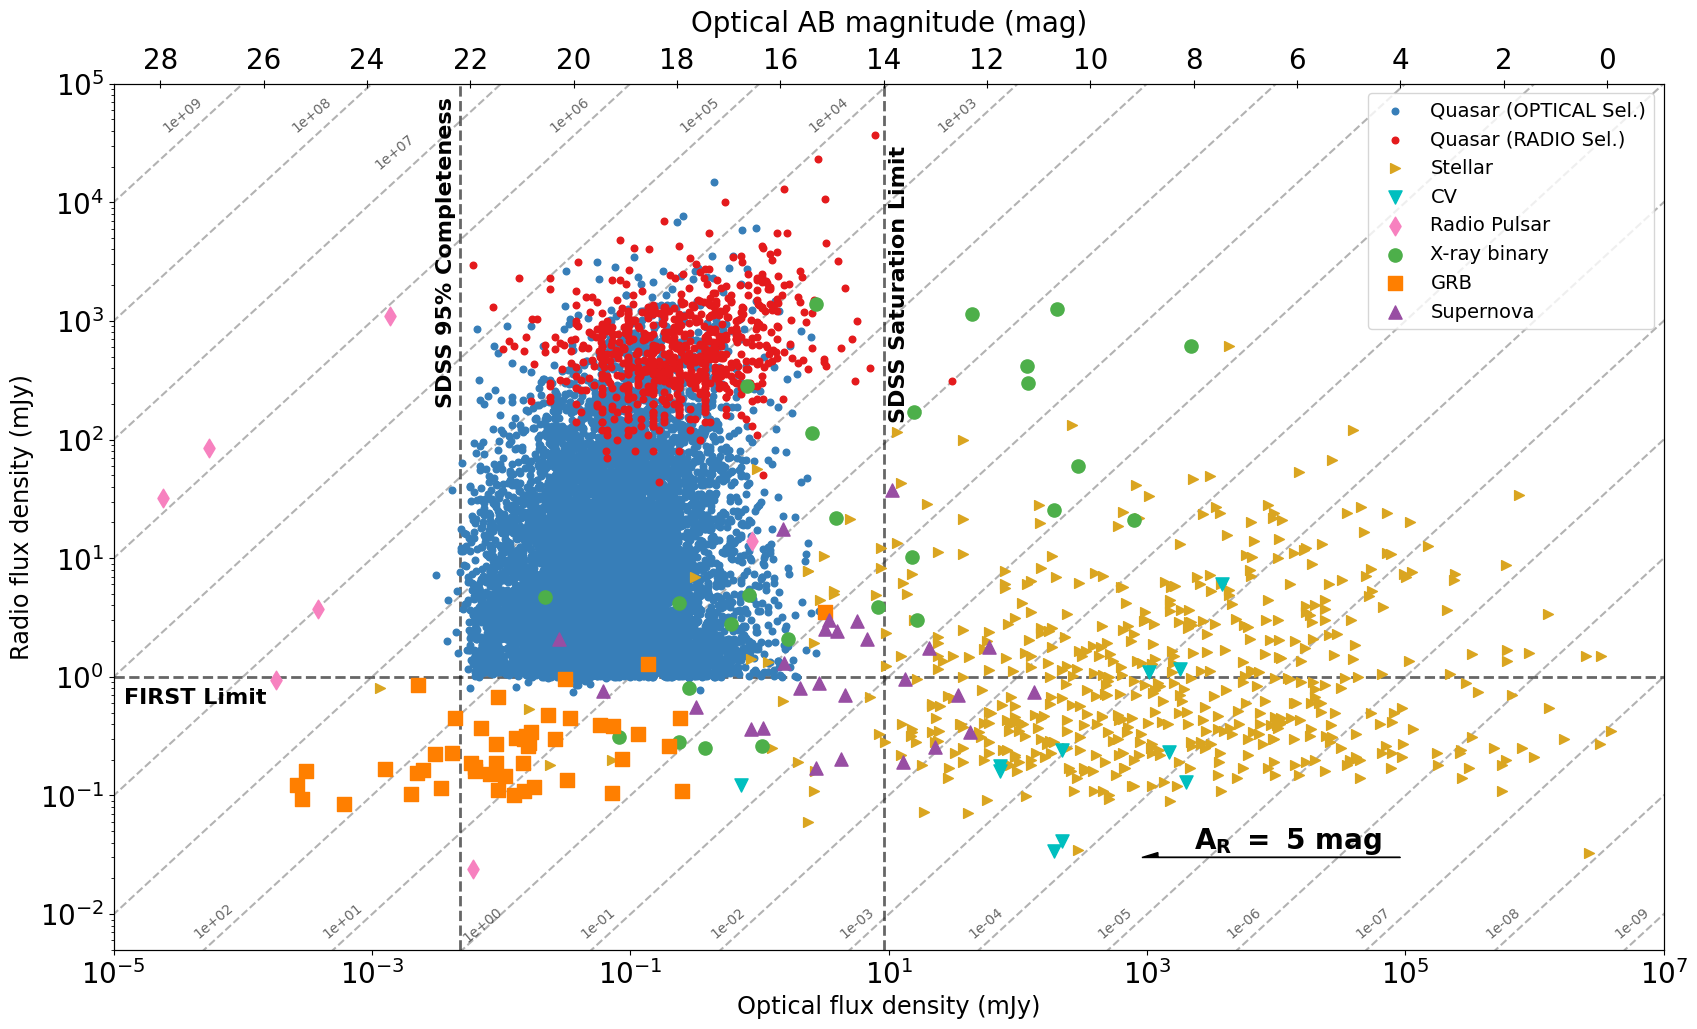
\includegraphics[width=0.9\textwidth]{ro_figure_1.png}
	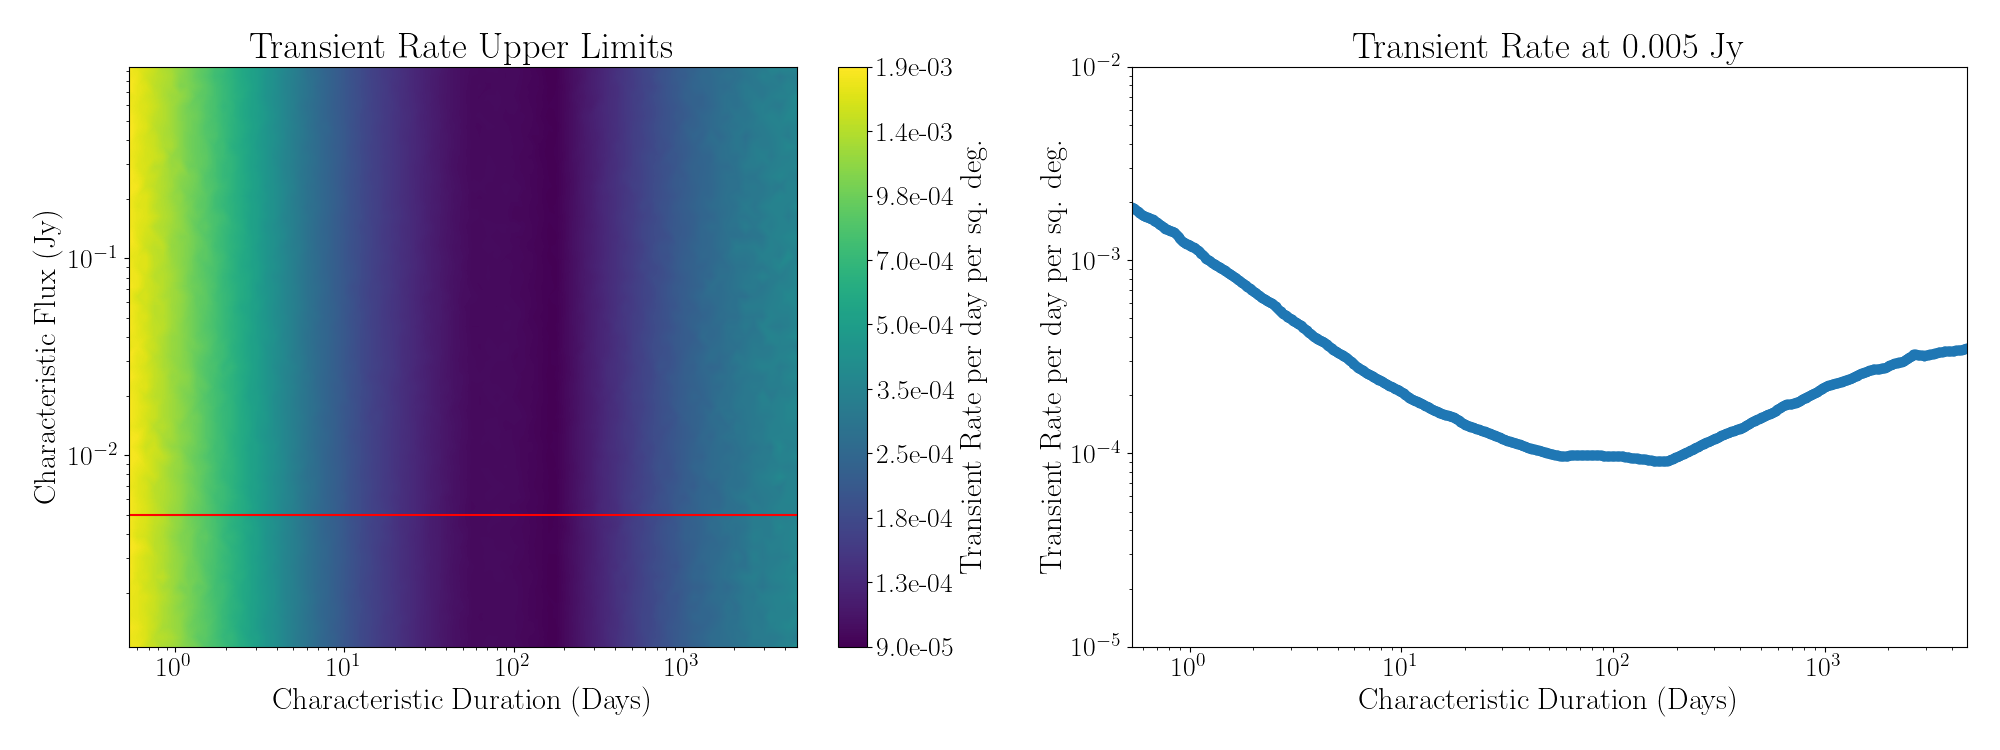
\includegraphics[width=\textwidth]{commensal2_30min.png}
	\caption{The left panel shows a surface plot with the transient rate upper limit calculated for a tophat light curve on the color axis and the transient duration and peak flux on the x and y axes respectively. The right panel shows the transient rate on the y axis for transient with a peak flux of 5 mJy. }
	\label{fig:transientrate}
 \end{figure}
\subsection{Conclusion}
\label{sec:conclusion3}
We have conducted a commensal search on short GRB and SN fields using methodology developed in~\citet{commensal1}. We found 13 sources of astrophysical origin with statistically significant variability. Of these sources, 7 of them have optical or near infrared data and appear to be associated with AGN. These 7 sources, along with another source, have redshifts in the DESI Legacy Imaging Survey \citep{10.1093...mnras...stac608}. We also find that 12 sources, including the aforementioned 8, have variability consistent with refractive interstellar scintillation. The variability of the remaining source could be intrinsic in nature. However, it could also be that the distance to the scattering screen used in calculating the expected refractive scintillation is about half of what is estimated. Finally, we place upper limits on the transient rate using this survey, and find that the upper limits we place on the transient rate is a factor of two better than the commensal search presented in \citet{commensal1}, likely due to more time spent on target and overall quality of the images.






\subsection{Acknowledgments}
The MeerKAT telescope is operated by the South African Radio Astronomy Observatory (SARAO), which is a facility of the National Research Foundation, an agency of the Department of Science and Innovation. We would like to thank the operators, SARAO staff and ThunderKAT Large Survey Project team.

We acknowledge use of the Inter-University Institute for Data Intensive Astronomy (IDIA) data intensive research cloud for data processing. IDIA is a South African university partnership involving the University of Cape Town, the University of Pretoria and the University of the Western Cape. We also acknowledge the computing resources provided on the High Performance Computing Cluster operated by Research Technology Services at the George Washington University.

This research has made use of the CIRADA cutout service at URL cutouts.cirada.ca, operated by the Canadian Initiative for Radio Astronomy Data Analysis (CIRADA). CIRADA is funded by a grant from the Canada Foundation for Innovation 2017 Innovation Fund (Project 35999), as well as by the Provinces of Ontario, British Columbia, Alberta, Manitoba and Quebec, in collaboration with the National Research Council of Canada, the US National Radio Astronomy Observatory and Australia’s Commonwealth Scientific and Industrial Research Organisation.

The ASKAP radio telescope is part of the Australia Telescope National Facility which is managed by Australia’s national science agency, CSIRO. Operation of ASKAP is funded by the Australian Government with support from the National Collaborative Research Infrastructure Strategy. ASKAP uses the resources of the Pawsey Supercomputing Research Centre. Establishment of ASKAP, the Murchison Radio-astronomy Observatory and the Pawsey Supercomputing Research Centre are initiatives of the Australian Government, with support from the Government of Western Australia and the Science and Industry Endowment Fund. We acknowledge the Wajarri Yamatji people as the traditional owners of the Observatory site. This paper includes archived data obtained through the CSIRO ASKAP Science Data Archive, CASDA (https://data.csiro.au).

This research has made use of the VizieR catalogue access tool, CDS, Strasbourg, France (DOI: 10.26093/cds/vizier). The original description of the VizieR service was published in 2000, A\&AS 143, 23.





\begin{figure}
	% 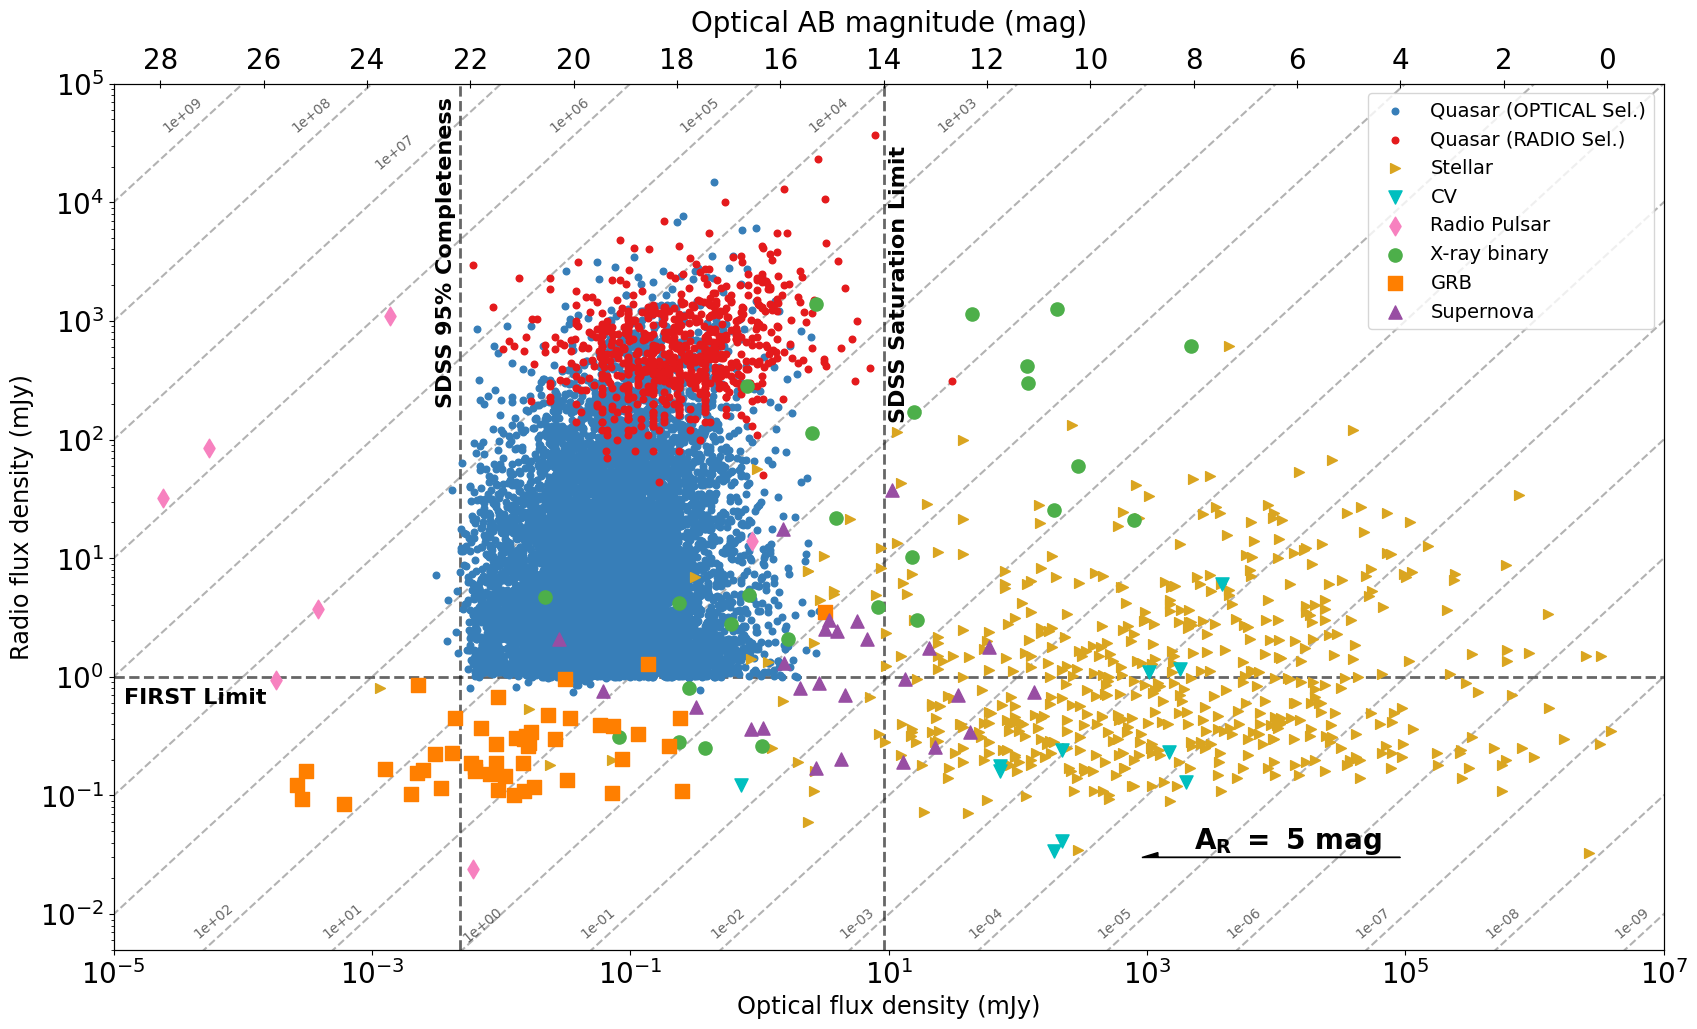
\includegraphics[width=0.9\textwidth]{ro_figure_1.png}
	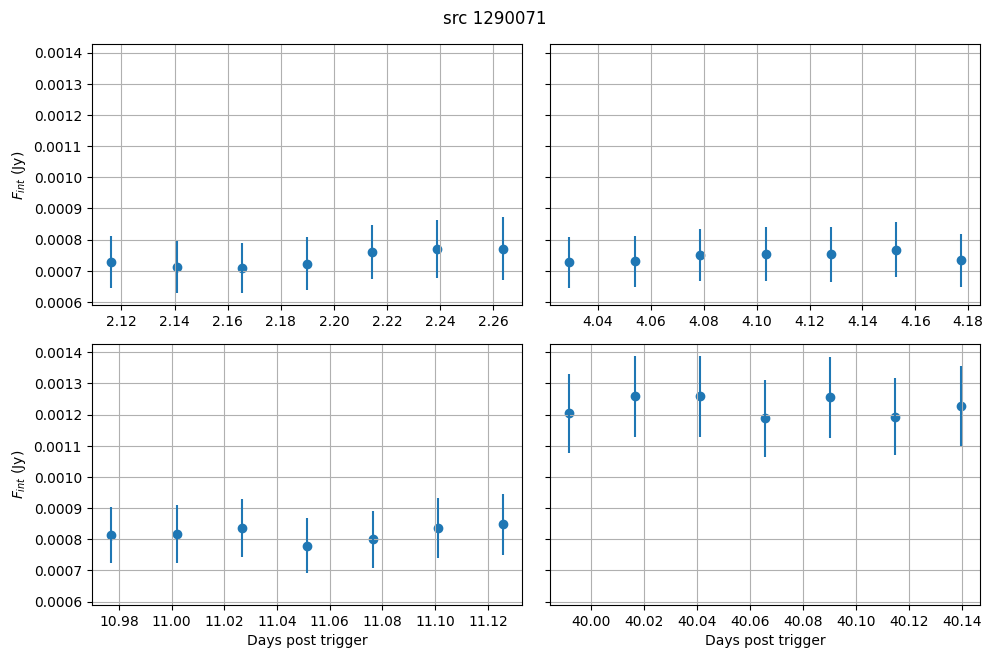
\includegraphics[width=\textwidth]{src1290071multi.png}
	\caption{A light curve showing all observations of source number 1290071. This source shows variability only on the observation-to-observation level. It also has radio counterparts and the variability timescale of around 30 days does not match the refractive scintillation timescale of around 60 days.}
	\label{fig:src1290071multi}
\end{figure}
\begin{figure}
	% 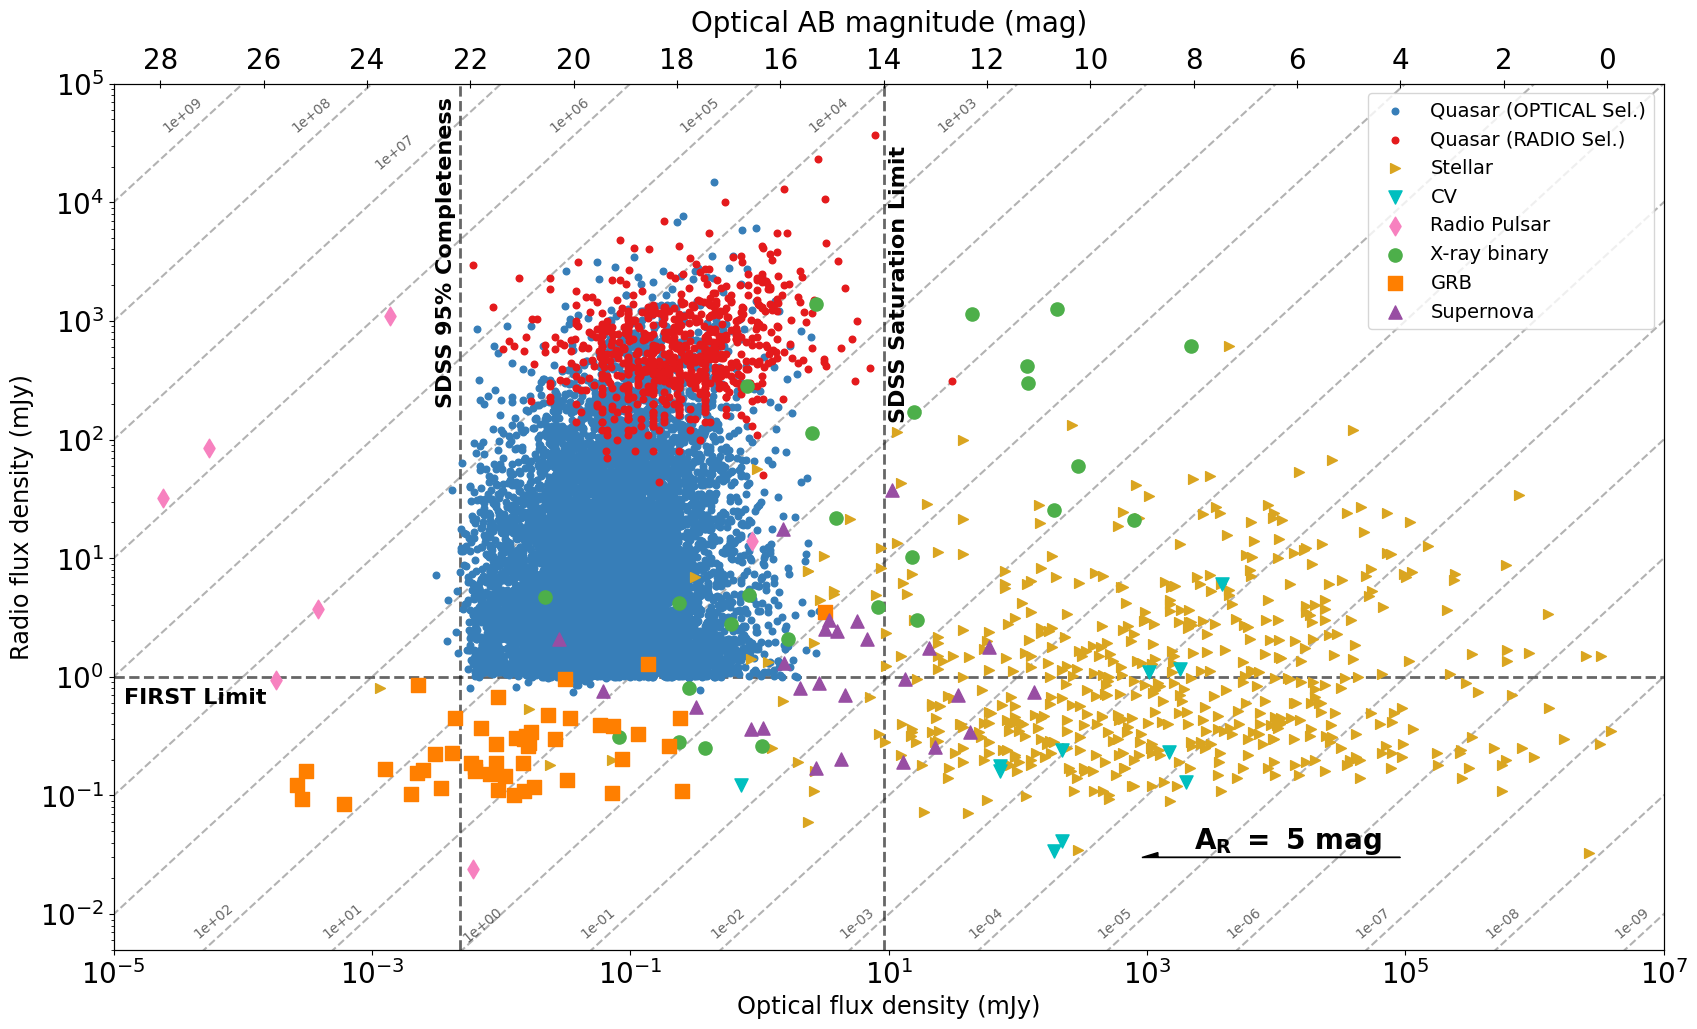
\includegraphics[width=0.9\textwidth]{ro_figure_1.png}
	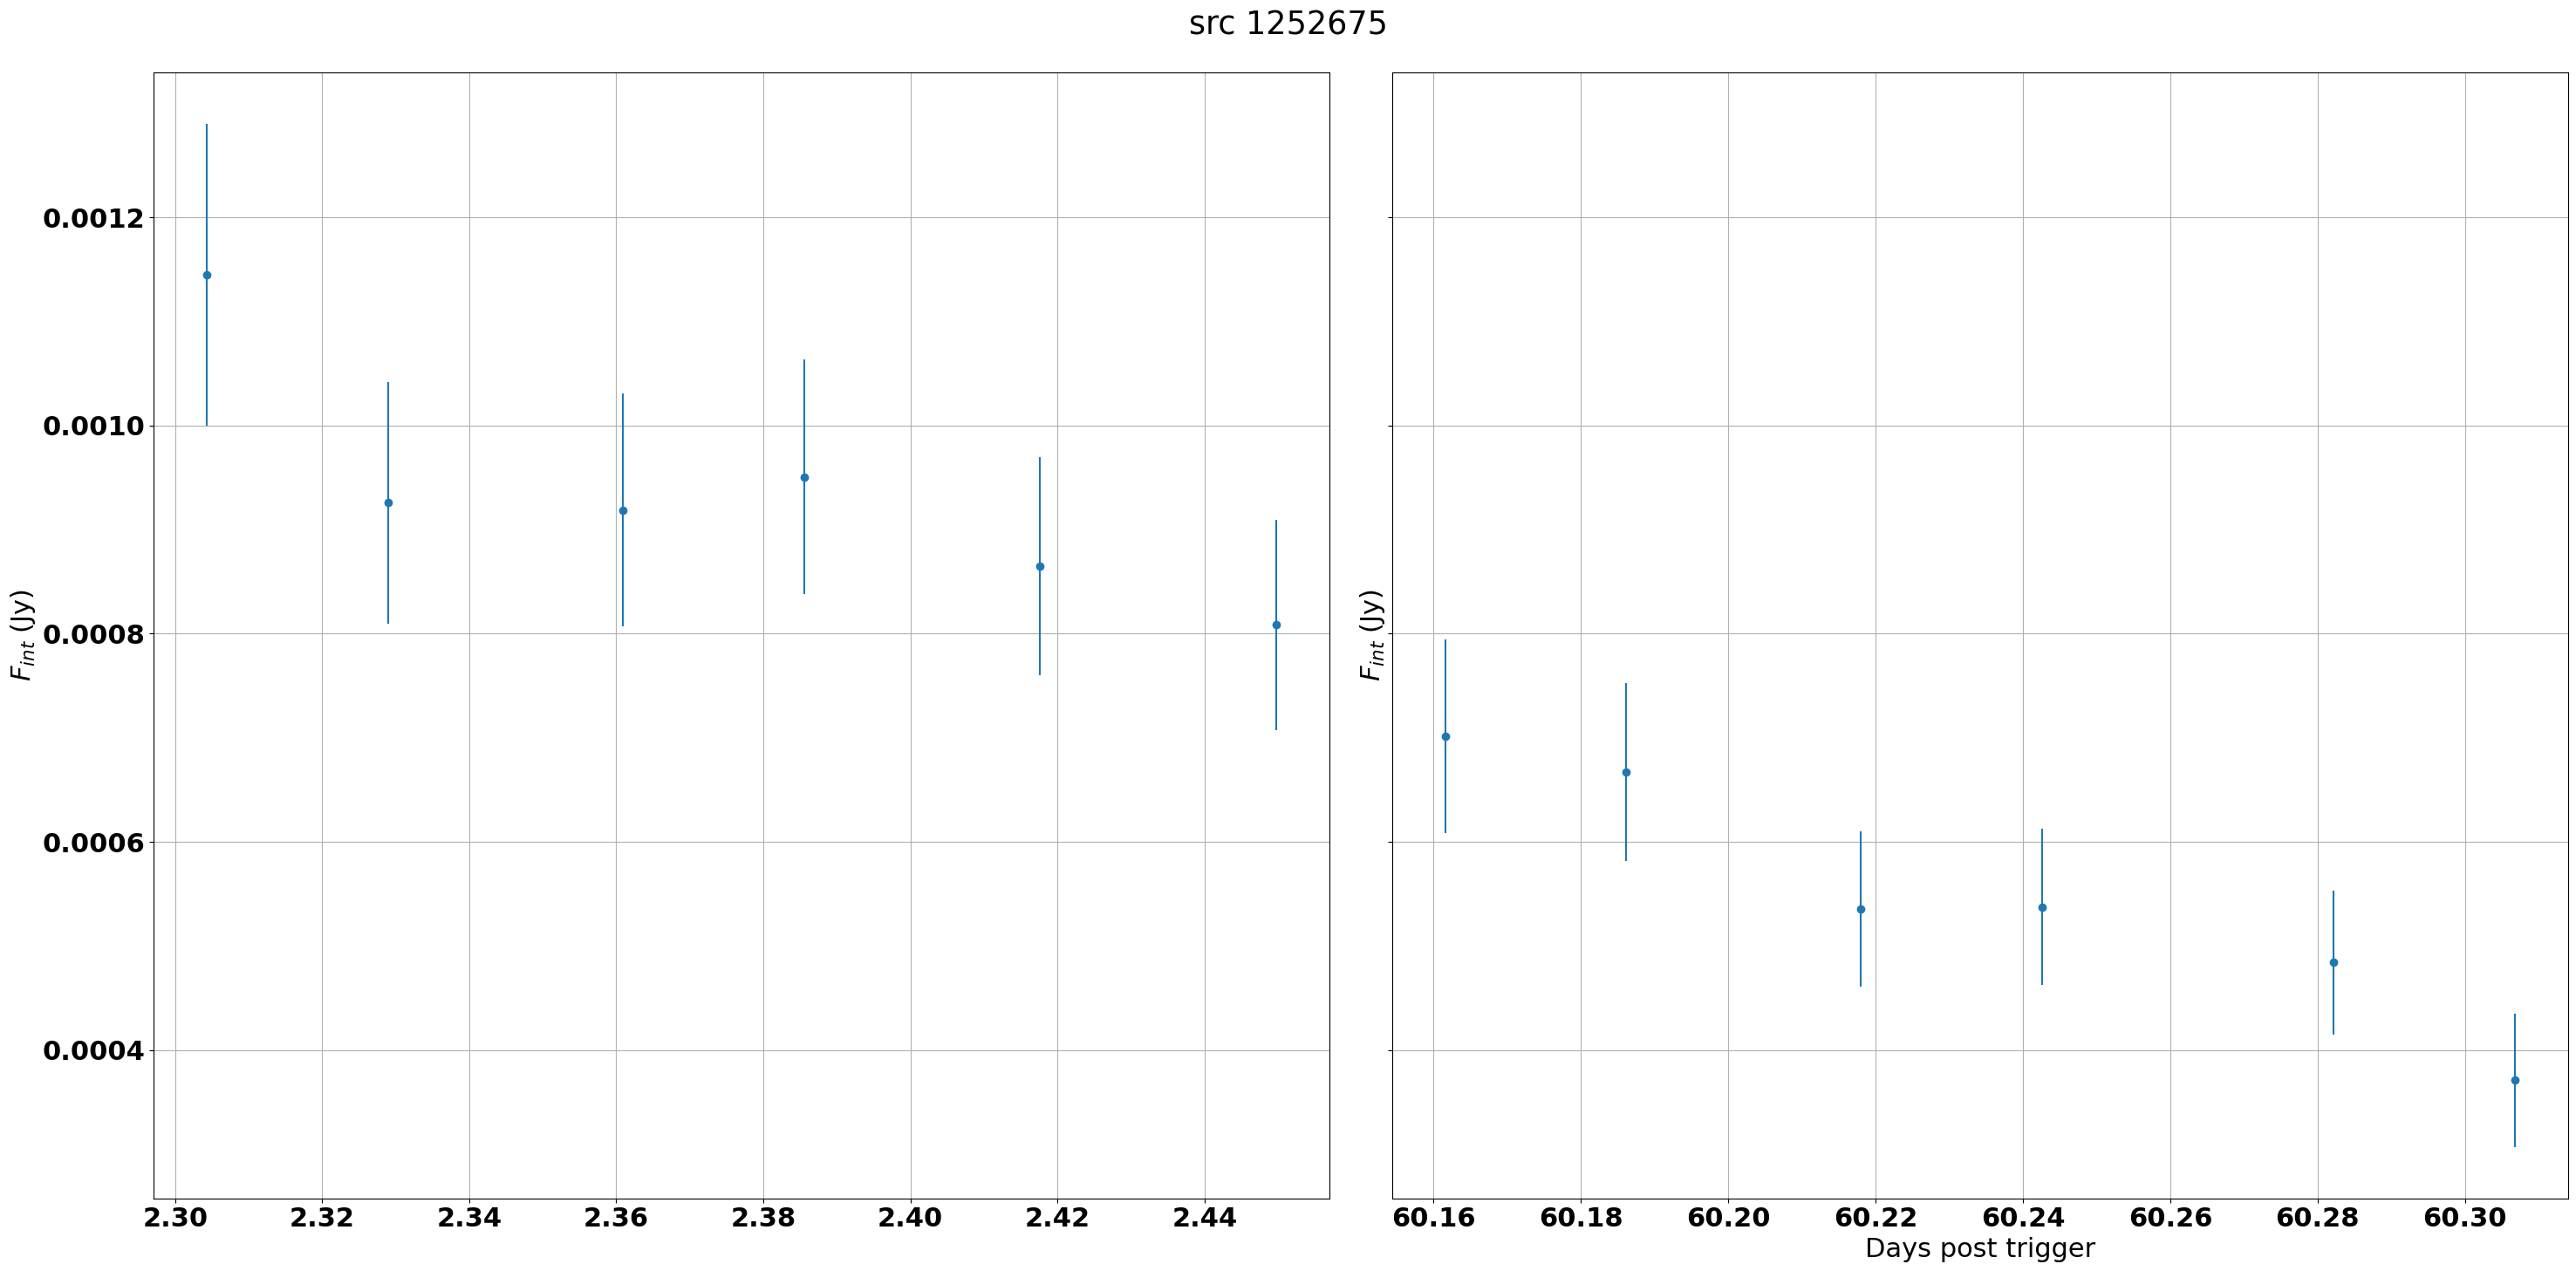
\includegraphics[width=\textwidth]{src1252675multi.png}
	\caption{Light curve for source 1252675. This source has radio counterparts.}
	\label{fig:src1252675multi}
\end{figure}
\begin{figure}
	% \includegraphics[width=0.9\textwidth]{ro_figure_1.png}
	\includegraphics[width=\textwidth]{src1260388multi.png}
	\caption{Light curve for source 1260388. This source has radio counterparts.}
	\label{fig:src1260388multi}
\end{figure}
\begin{figure}
	% \includegraphics[width=0.9\textwidth]{ro_figure_1.png}
	\includegraphics[width=\textwidth]{src1260578multi.png}
	\caption{Light curve for source 1260578. This source has radio counterparts..}
	\label{fig:src1260578multi}
\end{figure}
\begin{figure}
	% \includegraphics[width=0.9\textwidth]{ro_figure_1.png}
	\includegraphics[width=\textwidth]{src1267266multi.png}
	\caption{Light curve for source 1267266. This source has radio counterparts.}
	\label{fig:src1267266multi}
\end{figure}
\begin{figure}
	% \includegraphics[width=0.9\textwidth]{ro_figure_1.png}
	\includegraphics[width=\textwidth]{src1278651multi.png}
	\caption{Light curve for source 1278651. This source has upper limits from radio surveys.}
	\label{fig:src1278651multi}
\end{figure}
\begin{figure}
	% \includegraphics[width=0.9\textwidth]{ro_figure_1.png}
	\includegraphics[width=\textwidth]{src1279472multi.png}
	\caption{Light curve for source 1279472. This source has radio counterparts.}
	\label{fig:src1279472multi}
\end{figure}
\newpage
\section{Limits on Short GRBs from Radio Observations}

Gamma-ray bursts (GRBs) are among the most powerful explosive transients in the sky, accelerating electrons to extremely high Lorentz factors and emitting photons with up to TeV energies \citep[e.g.,][]{2019Natur.575..464A,2019Natur.575..459M}. These extreme sources can be divided into two varieties: long-soft and short-hard GRBs, based on the observed duration and spectral hardness of their initial gamma-ray emission \citep{1993ApJ...413L.101K}. Long GRBs are caused by massive stellar explosions \citep{1993ApJ...405..273W}, with nearby ones associated with supernovae \citep[e.g.,][]{2003Natur.423..847H}. Short GRBs are caused by binary mergers of compact objects \citep{1989Natur.340..126E}, with some of them associated with kilonovae \citep[e.g.,][]{2013Natur.500..547T} and one with a gravitational wave event \citep{2017ApJ...848L..12A}. Following the GRB prompt gamma-ray emission, irrespective of the progenitor, an afterglow is observed across the electromagnetic spectrum, due to the interaction between the ejected material and the surrounding medium \citep{1998ApJ...497L..17S,1999ApJ...523..177W,1999ApJ...520L..29C}.

Multi-wavelength observations of GRBs provide constraints on the physical parameters of the collimated GRB outflow, i.e., the jet, its surrounding medium, and the microphysics of the enhanced magnetic fields and accelerated electrons in the blast wave at the front of the jet \citep{1998ApJ...497L..17S}. Radio observations provide a particularly important role, since the synchrotron emission from GRB afterglows can be tracked and well defined over time, especially in the case of bright ones \citep[see, e.g.,][for a review]{2014PASA...31....8G}.

While radio detections of long GRB afterglows are becoming increasingly common, there are still very few detections of short GRB afterglows in radio. \citet{2015ApJ...815..102F} conducted a comprehensive study of the short GRB population and derived, using broadband modeling, limits on the physical parameters using flux measurements and limits from multi-wavelength observations including radio. The modeling from this study seems to suggest that the energetics of short GRBs and the particle density in their environment can be quite low, with densities as low as those found in the intergalactic medium, i.e., $10^{-6}$ cm$^{-3}$. Such low densities have been a point of debate \citep{2020MNRAS.495.4782O}. Furthermore, recent broadband modeling of a sample of both long and short GRBs, using state-of-the-art modeling and statistical techniques \citep{2022MNRAS.511.2848A}, indicate that the energy of the blast wave is similar in long GRBs and short GRBs, but that the difference in their observed gamma-ray energetics is due to differences in gamma-ray efficiency, while this efficiency is quite homogenenous among the population of long GRBs \citep{2016MNRAS.461...51B}. These debates in the literature, combined with a relatively small sample of short GRBs with radio detections \citep{2021ApJ...906..127F}, are a strong motivation to perform more radio studies of short GRBs.

Various afterglow models \citep[e.g.,][]{2002ApJ...568..820G,2012ApJ...749...44V} have been used to derive physical GRB parameters by fitting multi-wavelength observations across various observing frequencies and timescales. Since the physical parameter space is large and complex, some methods have been derived to pin down one or two of the parameters using just a few observables. For instance, one can use the peak in radio light curves and spectra to constrain parameters related to electron acceleration in these sources \citep{2017MNRAS.472.3161B}. In this study, the authors determine typical values for the fraction of the shock energy that goes into the population of accelerated electrons and establish a fairly narrow distribution for this parameter. \citet{2023MNRAS.518.1522D} follows up on this work by additionally constraining the fraction of electrons that gets accelerated by the blast wave and the minimum Lorentz factor of the distribution of accelerated electrons. While this was done for a large sample (almost 50) of long GRBs, this has not been applied to a sample of short GRB radio afterglows.

More radio detections of short GRB afterglows are needed to better understand the differences between the short and long GRB populations. In the Observations and Data Analysis section, we present an observing campaign of short GRBs with the MeerKAT observatory, as part of the ThunderKAT project \citep{2016mks..confE..13F}. In the Modeling Results and Host Galaxies section, we present the results of our multi-epoch observations of 7 short GRB fields, and use the flux measurements and limits to constrain some GRB parameters and their environments. We also use our sensitive observations to constrain star formation rates in likely host galaxies of some of the GRBs in our sample. In the following Discussion section, we discuss the implications of our measurements and limits on the GRB parameters, along with the next steps that need to be taken to build upon this study. Finally, we provide a brief summary and conclusions in the Conclusion.


\begin{deluxetable}{lllclll}
	\tablecolumns{7}
	\tablewidth{0pc}
	\tablecaption{A summary of all observations taken, forced measurements at the GRB afterglow location, and rms noise. $\Delta T$ is the time elapsed since the GRB trigger.\label{tab:observations}}
	\tablehead{ \colhead{GRB} & \colhead{RA} & \colhead {Dec} & \colhead{$\Delta T$} &        \colhead{RMS}  & \colhead{$F_{int}$} & \colhead{$F_{pk}$}\\
		\colhead{} & \colhead{(deg)}  & \colhead{(deg)} & \colhead{(days)} &        \colhead{($\mu$Jy) } &        \colhead{($\mu$Jy) } }
	\startdata
GRB200219A & 342.6384 & -59.1196 &   0.30 &  9 &   $31 \pm 13$ &      $29 \pm 7$ \\
GRB200219A & 342.6384 & -59.1196 &   2.21 &  7 &   $18 \pm 10$ &      $16 \pm 5$ \\
GRB200219A & 342.6384 & -59.1196 &   4.20 &  7 &   $31 \pm 10$ &      $30 \pm 6$ \\
GRB200219A & 342.6384 & -59.1196 &   8.27 &  8 &   $13 \pm 11$ &     $11 \pm 5$ \\
GRB200219A & 342.6384 & -59.1196 & 916.72 &  7 &   $19 \pm 10$ &      $17 \pm 5$ \\
GRB200411A &  47.6642 & -52.3176 &   1.12 &  7 &   $24 \pm 11$ &      $22 \pm 6$ \\
GRB200411A &  47.6642 & -52.3176 &   3.30 &  7 &   $52 \pm 11$ &      $51 \pm 8$ \\
GRB200411A &  47.6642 & -52.3176 &   7.13 &  6 &   $37 \pm 10$ &      $36 \pm 6$ \\
GRB200411A &  47.6642 & -52.3176 & 862.91 &  7 &   $35 \pm 10$ &      $34 \pm 6$ \\
GRB200522A &   5.6818 &  -0.2827 &   0.81 & 29 &   $6 \pm 52$ &       $-145 \pm 737$ \\
GRB200522A &   5.6818 &  -0.2827 &   1.77 & 30 &   $29 \pm 68$ &      $-24 \pm 32$ \\
GRB200522A &   5.6818 &  -0.2827 &   6.61 & 32 &   $24 \pm 60$ &      $-24 \pm 35$ \\
GRB200522A &   5.6818 &  -0.2827 &  14.61 & 32 &   $-20 \pm 64$ &     $46 \pm 83$ \\
GRB200522A &   5.6818 &  -0.2827 & 816.49 & 47 &   $9 \pm 77$ &       $-216 \pm 1095$ \\
GRB200907B &  89.0290 &   6.9062 &   0.27 & 13 &   $9 \pm 23$ &       $-9 \pm 13$ \\
GRB200907B &  89.0290 &   6.9062 &   2.30 & 12 &   $-9 \pm 26$ &      $17 \pm 30$ \\
GRB200907B &  89.0290 &   6.9062 &   6.29 & 12 &   $-2 \pm 25$ &      $117 \pm 970$ \\
GRB200907B &  89.0290 &   6.9062 &  17.32 & 12 &   $-4 \pm 26$ &      $54 \pm 208$ \\
GRB200907B &  89.0290 &   6.9062 & 710.44 & 15 &   $-2 \pm 27$ &      $109 \pm 760$ \\
GRB210323A & 317.9472 &  25.3692 &   1.35 &  9 &   $26 \pm 14$ &      $23 \pm 7$ \\
GRB210323A & 317.9472 &  25.3692 &   3.34 &  9 &   $14 \pm 14$ &      $10 \pm 6$ \\
GRB210323A & 317.9472 &  25.3692 &   8.33 &  8 &   $15 \pm 13$ &      $11 \pm 6$ \\
GRB210323A & 317.9472 &  25.3692 &  11.72 &  9 &   $19 \pm 15$ &      $15 \pm 7$ \\
GRB210323A & 317.9472 &  25.3692 & 517.93 &  9 &   $15 \pm 14$ &      $11 \pm 6$ \\
GRB210919A &  80.2546 &   1.3120 &   1.05 & 17 &   $-7 \pm 32$ &      $43 \pm 119$ \\
GRB210919A &  80.2546 &   1.3120 &   5.11 & 18 &   $-9 \pm 30$ &      $24 \pm 45$ \\
GRB210919A &  80.2546 &   1.3120 & 335.20 & 31 &   $-9 \pm 50$ &      $80 \pm 248$ \\
GRB210919A &  80.2546 &   1.3120 &   8.05 & 18 &   $-32 \pm 32$ &     $-21 \pm 12$ \\
GRB220730A & 225.0143 & -69.4959 &   2.12 &  8 &   $21 \pm 17$ &      $16 \pm 8$ \\
GRB220730A & 225.0143 & -69.4959 &   4.03 &  7 &   $4 \pm 13$ &       $-11 \pm 21$ \\
GRB220730A & 225.0143 & -69.4959 &  10.98 &  8 &   $6 \pm 16$ &       $-8 \pm 13$ \\
GRB220730A & 225.0143 & -69.4959 &  39.99 &  9 &   $6 \pm 11$ &       $-2 \pm 3$ \\
	\enddata
\end{deluxetable}


\subsection{Observations and Data Analysis}

The aim of this project was to observe short GRBs, mainly detected with the Neil Gehrels Swift Observatory \citep{2004ApJ...611.1005G}, that had follow-up observations in at least one other waveband (X-rays, UV, optical and/or near-infrared). The observing campaign started in early 2020, with the last observations presented in this paper taken in August 2022. We performed multi-epoch observations of 7 GRBs, spanning days to weeks, and in 6 cases even years (the 7th GRB occurred in July 2022). This resulted in 32 total observations for our sample of 7 short GRBs, all with a central frequency of 1.3~GHz, and the observing details and results are summarized in Table~\ref{tab:observations}. All observations were approximately 4 hours in length, resulting in $1-\sigma$ noise levels down to $7-9\,\mu$Jy in several fields. In some cases the image noise was significantly higher, up to a few tens of $\mu$Jy, due to bright sources in the field causing strong artifacts.

Each observation was processed using the ProcessMeerKAT pipeline \citep{pminprep} for calibration. The imaging was performed with Common Astronomy Software Applications (CASA) \citep{2022arXiv221002276T} using the task tclean. An initial shallow image was made, then self-calibration and refined flagging for radio-frequency interference was performed, followed by making a final, deep image. W-projection with 128 w-projection planes were used to correct for the non-coplanar baselines. The multi-term multi-scale imaging algorithm was used with 2 Taylor series terms and at least three different scales, always including 0, 5, and 15. 

Even though the vast majority of our observations resulted in deep images, none of the ones presented here had significant detections at the GRB location. Some of the observations resulted in possible detections of a host galaxy, which will be discussed in the next section. During our campaign, the short GRB~210726A was also observed, resulting in some detections, which will be presented as part of a multi-wavelength study in~\citep{grb210726ainprep}. 

Given the non-detections of the GRBs in our sample, forced flux measurements at the GRB location were performed with the LOFAR transients pipeline \citep[TraP;][]{2015A&C....11...25S} using standard parameter settings, and the image noise was also measured with the TraP. The light curves of the forced peak flux measurements along with $3\sigma$ upper limits are shown in Figure~\ref{fig:allmeasurements}. 

Note that almost all the forced peak flux measurements for GRB~200411A are higher than the $3\sigma$ upper limits because the host galaxy, which is offset from the GRB position and constant in time, is contributing to the flux at that position. Figure~\ref{fig:GRB200411Afield} shows all observations of the GRB~200411A location. The forced fit location is marked with a red cross. The location of the GRB is slightly offset from another source marked with a blue dot. We searched Vizier~\citep{vizier} for a counterpart to this source and found that it corresponds to a source that is classified as a ``high-confidence galaxy'' in the Dark Energy Survey Data Release 2~\citep{Abbott_2021}. Therefore, the flux measured from this GRB is from this galaxy, which is likely its host galaxy, and not from the GRB afterglow.





\begin{figure}
	% To include a figure from a file named example.*
	% Allowable file formats are eps or ps if compiling using latex
	% or pdf, png, jpg if compiling using pdflatex
	\includegraphics[width=\textwidth]{plotboth.png}
	\caption{All forced measurements of peak flux are shown with blue circles and the 3 sigma upper limits based on the rms noise are shown in orange triangles.}
	\label{fig:allmeasurements}
\end{figure}

\begin{figure}
	% To include a figure from a file named example.*
	% Allowable file formats are eps or ps if compiling using latex
	% or pdf, png, jpg if compiling using pdflatex
	\includegraphics[width=\textwidth]{GRB200411Aff.png}
	\caption{All observations of GRB 200411A are shown with the forced fit location marked with a red ``x''. Note the nearby source marked with a blue dot. }
	\label{fig:GRB200411Afield}
\end{figure}

\subsection{Modeling Results and Host Galaxies}
~\label{sec:methodandresult5}

In this section we put our results in the context of GRB modeling and host galaxy studies.
\subsubsection{Constraining GRB Afterglow Physics}

We use our deep MeerKAT observations to constrain some of the physical parameters for our sample of short GRBs. One approach would be to perform multi-wavelength modeling covering a wide range in timescales and frequencies, but the amount of data available for this is limited. The reason for this is two-fold: (1) short GRBs are typically faint across the electromagnetic spectrum, and that is also true for the GRBs in our sample; and (2) due to the global COVID pandemic, there were limited observations, in particular in the optical, during a significant fraction of our campaign. Therefore, we focus here on the MeerKAT observations and what can be learned from the deep limits we obtained on the radio brightness.

We model our MeerKAT observations by comparing the $3\sigma$ upper limits to the theoretical expectations of peaks in radio light curves and spectral energy distributions \citep{2017MNRAS.472.3161B,2023MNRAS.518.1522D}. For every observation, we can consider the measured upper limit to be a limit on the theoretical peak flux if it would be at that time and frequency. Given the quasi-logarithmic spacing of our observations, similar flux limits at various times for a given GRB, and the power-law flux evolution of GRB afterglows, it is very unlikely that we would have missed any radio peak in the gaps between our observations, except possibly for the observations between a few weeks and one or two years after the GRB. 

For every observation we calculate the $\Psi$ parameter from \citet{2017MNRAS.472.3161B} and \citet{2023MNRAS.518.1522D}, which uses the observing frequency, observation time, peak flux (for which we use the $3\sigma$ upper limits), redshift, luminosity distance, and isotropic-equivalent gamma-ray energy. We show the redshift and gamma-ray energy values used, and their references, in Table~\ref{tab:GRBprops}. For the two GRBs without a known redshift, we use the average redshift of the other 5 GRBs. The luminosity distance of each GRB was calculated using \citet{2006PASP..118.1711W}. The upper limits on the peak flux result in lower limits on the $\Psi$ parameter, which are shown in Table~\ref{tab:psiobs}. We also show a histogram of the lower limits on $\Psi$ in Figure~\ref{fig:psiobshist}. We note that we are using the $\Psi$ equations for a homogeneous medium, since that is the typically assumed environment of a short GRB (rather than a massive stellar wind, which one may expect for long GRBs). This distribution of lower limits on $\Psi$ can be compared to the distribution of measured $\Psi$ values for a large sample of long GRBs \citep{2023MNRAS.518.1522D}, and the implications of this are discussed in the next section.
\newgeometry{margin=1.25in} % modify this if you need even more space
\begin{landscape}
\begin{deluxetable}{lllll}
	\tablecolumns{5}
	\tablewidth{0pc}
	\tablecaption{This table shows the observational parameters used and their sources. For GRBs without a known redshift, the average of all of the other redshifts is used: 0.438.
				\label{tab:GRBprops}}
	\tablehead{
			\colhead{GRB} & \colhead{Redshift} & \colhead{}  &     \colhead{$E_{\gamma,iso}$} & \colhead{} \\
    & & & \colhead{(erg)}& \\} 
	\startdata
	GRB200219A & 0.484 &  \citet{2022MNRAS.512.3662D} &$3.74\times10^{51}$ & \citet{2020GCN.27226....1S}\\
	GRB200411A & 0.6 & \citet{2022MNRAS.515.4890O} &$7.17\times10^{50}$ & \citet{2020GCN.27543....1B}\\
	GRB200522A & 0.554 & \citet{2020GCN.28038....1D} &$1.39\times10^{50}$ & \citet{2020GCN.27793....1U} \\
	GRB200907B &  &  &$1.28\times10^{50}$ & \citet{2020GCN.28398....1K}\\
	GRB210323A & 0.37 & \citet{2021GCN.29717....1D} &$2.18\times10^{50}$ & \citet{2021GCN.29713....1F} \\
	GRB210919A & 0.27 & \citet{2021GCN.30934....1O} &$5.53\times10^{49}$ & \citet{2022GCN.31566....1M} \\
	GRB220730A &  &  &$4.51\times10^{51}$ & \citet{2022GCN.32439....1F} \\    
	 \enddata
\end{deluxetable}
\end{landscape}
\restoregeometry
 \doublespacing
%\begin{deluxetable}{lll}
%	\tablecolumns{3}
%	\tablewidth{0pc}
%	\tablecaption{This table shows the observational parameters used and their sources. For GRBs without a known redshift, the average of all of the other redshifts is used: 0.438.
%		\label{tab:GRBprops}}
%	\tablehead{
%		\colhead{GRB} & \colhead{Redshift} &        \colhead{$E_{\gamma,iso}$} \\} 
%	\startdata
%	GRB200219A & 0.484\tablenotemark{a} &$3.74\times10^{51}$\tablenotemark{b}\\
%	GRB200411A & 0.6\tablenotemark{c} &$7.17\times10^{50}$\tablenotemark{d}\\
%	GRB200522A & 0.554\tablenotemark{e} &$1.39\times10^{50}$\tablenotemark{f} \\
%	GRB200907B &   &$1.28\times10^{50}$\tablenotemark{g}\\
%	GRB210323A & 0.37\tablenotemark{h} &$2.18\times10^{50}$\tablenotemark{i} \\
%	GRB210919A & 0.27\tablenotemark{j} &$5.53\times10^{49}$\tablenotemark{k} \\
%	\enddata
%	\tablenotetext{a}{\citet{2022MNRAS.512.3662D}}
%	\tablenotetext{b}{\citet{2020GCN.27226....1S}}
%	\tablenotetext{c}{\citet{2022MNRAS.515.4890O}}
%	\tablenotetext{d}{\citet{2020GCN.27543....1B}}
%	\tablenotetext{e}{\citet{2020GCN.28038....1D}}
%	\tablenotetext{f}{\citet{2020GCN.27793....1U}}
%	\tablenotetext{g}{\citet{2020GCN.28398....1K}}
%	\tablenotetext{h}{\citet{2021GCN.29717....1D}}
%	\tablenotetext{i}{\citet{2021GCN.29713....1F}}
%	\tablenotetext{j}{\citet{2021GCN.30934....1O}}
%	\tablenotetext{k}{\citet{2022GCN.31566....1M}}
%\end{deluxetable}

\begin{deluxetable}{llll}
	\tablecolumns{4}
	\tablewidth{0pc}
	\tablecaption{Lower limits on $\Psi$ calculated from 3$\sigma$ upper limits on the GRB afterglow. Note that the observations for which $\Psi$ parameter is calculated only includes those before 100 days post-trigger since it is intended to be calculated at the peak of the light curve. \label{tab:psiobs}}
	\tablehead{ \colhead{GRB} & \colhead{$\Delta T$ Post-Burst} &        \colhead{3$\sigma$ upper limit }  & \colhead{$\text{Log}10(\psi) >$} \\
	\colhead{} & \colhead{(days)} &        \colhead{(mJy) }  & \colhead{} }
	\startdata
 		GRB200219A &   0.297282 &  0.033596 & -1.639143 \\
		GRB200219A &   2.211832 &  0.023745 & -0.910105 \\
		GRB200219A &   4.196984 &  0.033196 & -0.774220 \\
		GRB200219A &   8.270155 &  0.022845 & -0.472136 \\
		GRB200411A &   1.118673 &  0.021102 & -1.390580 \\
		GRB200411A &   3.302272 &  0.019760 & -1.023731 \\
		GRB200411A &   7.132912 &  0.018021 & -0.752891 \\
		GRB200522A &   0.811652 &  0.087168 & -1.942288 \\
		GRB200522A &   1.773361 &  0.089213 & -1.692754 \\
		GRB200522A &   6.613219 &  0.095566 & -1.278981 \\
		GRB200522A &  14.607036 &  0.096882 & -1.023837 \\
		GRB200907B &   0.268053 &  0.037670 & -2.039425 \\
		GRB200907B &   2.298481 &  0.035106 & -1.324206 \\
		GRB200907B &   6.290605 &  0.035754 & -1.000237 \\
		GRB200907B &  17.319491 &  0.037105 & -0.678410 \\
		GRB210323A &   1.354090 &  0.026490 & -0.998830 \\
		GRB210323A &   3.344351 &  0.027434 & -0.711938 \\
		GRB210323A &   8.326125 &  0.024341 & -0.388861 \\
		GRB210323A &  11.723675 &  0.027249 & -0.301901 \\
		GRB210919A &   1.046809 &  0.052225 & -1.501705 \\
		GRB210919A &   5.108056 &  0.052874 & -0.988095 \\
		GRB210919A &   8.047582 &  0.054287 & -0.845765 \\
		GRB220730A &   2.116177 &  0.024517 & -1.053949 \\
		GRB220730A &   4.029109 &  0.022107 & -0.821736 \\
		GRB220730A &  10.977102 &  0.023876 & -0.511991 \\
		GRB220730A &  39.991887 &  0.025800 & -0.107710 \\
\enddata
\end{deluxetable}


\begin{figure}
	% To include a figure from a file named example.*
	% Allowable file formats are eps or ps if compiling using latex
	% or pdf, png, jpg if compiling using pdflatex
	\includegraphics[width=\columnwidth]{psiobshist.png}
	\caption{A histogram of lower limits on the $\Psi$ parameter from all measurements taken before 100 days post-trigger.}
	\label{fig:psiobshist}
\end{figure}



\subsubsection{Constraining Host Galaxy Star Formation Rates}
While we do not have significant detections of the 7 GRBs presented here, our observations result in detections of many other sources in the images, including some steady sources very nearby the GRB location. Given that many short GRBs reside in the outskirts or possibly even outside of their host galaxy, we explored the possibility that some of these nearby sources are associated with the respective host galaxies. For 5 GRBs in our sample, host galaxy locations in detailed optical images have been published and have no serious image quality issues affecting source measurement; for those sources we give the MeerKAT location and peak flux in Table~\ref{tab:GRBhostSFR}. The fluxes were measured in deep combined images of each field (12 to 16 hours of observing time in total for each field), by force fitting the flux at the host galaxy location using the TraP. In 4 of the 5 cases we have a $\gtrapprox3\sigma$ detection, except for GRB~200907B, in which case we show the $3\sigma$ upper limit.

There are various possible reasons for, and contributions to, the 1.3~GHz flux measured for these GRB host galaxies. The emission is typically dominated by two components: thermal bremsstrahlung around star-forming regions, and non-thermal synchrotron emission from cosmic-ray electrons accelerated in the galaxy's magnetic field. The latter is most dominant at low radio frequencies and can be related to the supernova rate in a galaxy, and through the supernova rate to the star formation rate. We can estimate the star formation rate in each host galaxy from the measured flux, using the formalism and equations from \citet{2011ApJ...737...67M}; and the results are shown in Table~\ref{tab:GRBhostSFR} as well. These star formation rates may be higher than star formation rates that can be derived from other observations in for instance the optical, because the radio observations provide a tracer that is unobscured by dust. However, we will consider the star formation rates in Table~\ref{tab:GRBhostSFR} to be upper limits, since there may be other contributions to the observed radio flux that are not taken into account in the star formation rate estimates we made.
\begin{deluxetable}{lrrrr}
\tablecolumns{5}
\tablewidth{0pc}
\tablecaption{GRB host galaxy locations, forced fit flux measurements (and one $3\sigma$ upper limit) from deep combined images, and star formation rates if the measured radio flux were from star formation activity.\label{tab:GRBhostSFR}}
\tablehead{
	\colhead{GRB} & \colhead{RA} & \colhead{Dec}  & \colhead{$F_{peak}$}  & \colhead{SFR } \\
    & \colhead{(deg)} & \colhead{(deg)} & \colhead{($\mu$Jy)} & \colhead{ ($M_{\odot}/yr$) } \\
	}
\startdata
    GRB200219A\tablenotemark{a,b}  & 342.63795 & -59.11988  & $20\pm4$  &$12\pm2$\\
GRB200411A\tablenotemark{a,b} & 47.66306 & -52.31654 & $46\pm3$ &$48\pm3$\\
GRB200907B\tablenotemark{b} & 89.02896 & 6.90629  & $<36$   &$<17$\\
GRB210323A\tablenotemark{b} & 317.94717 & 25.36944  & $18\pm6$  &$2\pm2$\\
GRB210919A\tablenotemark{a,b} & 80.25814 & 1.31112  & $67\pm16$  &$11\pm2$\\
\enddata
\tablenotetext{a}{\citet{2021AAS...23723503S}}
\tablenotetext{b}{\citet{2022ApJ...940...56F}}
\end{deluxetable}
%\begin{table*}
%	\caption{This table shows the GRB host locations, their forced flux measurement, 3 sigma limits from the combined images, and star formation rates if the flux were from star formation activity. The four hosts shown below are those that are detected with at least two sigma significance. The host of GRB 200907B is not detected and a 3$\sigma$ upper limit is given. }
%	\label{tab:GRBhostSFR}
%	\begin{tabular}{lrrrrr}
%		\hline
%		GRB & RA & Dec & & $F_{pk}$ ($\mu$Jy)  & SFR ($M_{\odot}/yr$)\\
%		\hline
%		GRB200219A & 342.63795 & -59.119883 & \citet{2021AAS...23723503S,2022ApJ...940...56F} & $20\pm4$  &12\\
%		GRB200411A & 47.663062 & -52.31654 & \citet{2021AAS...23723503S,2022ApJ...940...56F} & $46\pm3$ &48\\
%		GRB200907B & 89.028962 & 6.906288 & \citet{2022ApJ...940...56F} & <36   &<17\\
%		GRB210323A & 317.947167 & 25.369441 & \citet{2022ApJ...940...56F} & $18\pm6$  &2\\
%		GRB210919A & 80.258142 & 1.311117 & \citet{2021AAS...23723503S,2022ApJ...940...56F} & $67\pm16$  &11\\
%	\end{tabular}
%\end{table*}

% Make section referencing Murphy et al 2015 and their method of calculating SFRs. Need to make table with host galaxy positions and SFRs, need to cite the host galaxy positions. Also mention the measurement was a forced measurement at the host galaxy location of the deep image using TraP. 

\subsection{Discussion}
\label{sec:discussion4}

%%% This subsection on SFRs is really lacking. It really just says: we don't have anything to say, look at our measurements and make your own conclusions. For this reason, 
%%% it's not really even worth mentioning. There might be other things to say here, but I lack the knowledge to add them. Perhaps more can be added after we get the ATCA data? 
%%% Let me know what you think. 
% \subsection{Star Formation Rates}
% The star formation rates reported here are all reasonable values that could imply that the flux in the galaxy is due to star formation. However, without further analysis of flux measurements of these galaxies in other wavelengths only limited information can be gleaned about the host properties. Further studies comparing the values reported here with other reported measurements and measurements from multiwavelength catalogs may yield some interesting discoveries about the host galaxies of short gamma-ray bursts. This kind of undertaking would merit its own paper and is beyond the scope of this study. 
\subsubsection{Comparison with Other Studies}
Comparing our upper limits with the upper limits in, for instance,~\citet{2015ApJ...815..102F} and \citet{2021ApJ...906..127F} shows that our limits are about as deep as the deepest ones in other short GRB studies; and in fact, our limits are close to many of the low-significance detections of some short GRBs. Our observations are complementary to those from other studies, since our observations are in the L-band, i.e., at 1.3~GHz. Furthermore, since we carry out our multi-epoch observations to about one month, no matter if the GRB was detected or not in earlier observations, we are able to narrow down the observational parameter space more strongly.

For most of the short GRBs with detections, the peak of the radio emission in the C- or X-band, $\sim5$ or 9~GHz respectively, is within the first week \citep{2021ApJ...906..127F}. That peak should have been caught in L-band observations out to about 1 month after the initial gamma-ray trigger, so our sample should not be missing such a light curve peak. We note that we did not detect GRB~200522A, which was detected at higher radio frequencies \citep{2021ApJ...906..127F}, but this was due to a significantly higher noise level in our MeerKAT images because of a couple of bright sources in the field; and at more typical noise levels, as achieved for most of the other GRB fields, we would expect to have detected this source at 1.3~GHz.


\subsubsection{Implications on GRB Parameters and Environments}

As laid out in the Modeling Results and Host Galaxies section, our deep upper limits can be used to constrain some of the physical parameters that can be derived from peaks in radio light curves and spectral energy distributions. When comparing the $\Psi$ values and distributions from \citet{2017MNRAS.472.3161B} and \citet{2023MNRAS.518.1522D} with our lower limits on $\Psi$, as shown in Table~\ref{tab:psiobs} and Figure~\ref{fig:psiobshist}, it can be seen that our lower limits for the short GRBs are about the same as the detections for a large long GRB sample. This means that either our noise levels are very close to what is needed for having detections of these short GRBs at 1.3~GHz, or the physical parameters in short GRBs are different than those for long GRBs. We will first discuss the latter option, and in the next subsection we will further discuss radio detectability of short GRBs.

The value of $\Psi$ strongly depends on two parameters related to electron acceleration: it has a linear dependence with the fraction of shock energy in electrons, $\epsilon_{\rm{e}}$, and is proportional to $\xi_{\rm{e}}^{-3/2}$, with $\xi_{\rm{e}}$ being the fraction of electrons that gets accelerated into a power-law distribution of energies. Both of these physical parameters are efficiency factors related to how relativistic shocks accelerate electrons. Since both long and short GRBs have relativistic shocks at the front of their jets, and the microphysics of this process should be similar for all relativistic shocks, it would be unexpected for $\epsilon_{\rm{e}}$ and $\xi_{\rm{e}}$ to be very different for short and long GRBs. Therefore, we will explore other physical parameters that may be different for the two GRB classes.

While $\Psi$ depends strongly on $\epsilon_{\rm{e}}$ and $\xi_{\rm{e}}$, it depends weakly on other physical parameters. Most notably, $\Psi$ depends on the gamma-ray efficiency $\epsilon_{\gamma}$ and the circumburst density $n_0$ as $\Psi_{ISM}\propto n_0^{-1/4} ((1-\epsilon_{\gamma})/\epsilon_{\gamma})^{-1/4}$. 
Previous studies have presented conflicting conclusions on the typical values of the gamma-ray efficiency of GRBs and whether they differ significantly between long and short bursts. Some studies \citep{10.1111/j.1365-2966.2006.10280.x,10.1093/mnras/stv2033,10.1093/mnras/stw1331} suggest that $\epsilon_{\gamma}$ is always approximately 0.15. However, based on multi-wavelength modeling of a sample of long and short GRBs, \citet{2022MNRAS.511.2848A} find that the gamma-ray efficiency of short GRBs is significantly lower than for long GRBs, potentially by orders of magnitude. Deep radio observations could potentially distinguish between these two possibilities. If we look again at the parameter scalings for $\Psi$, we can see that $\Psi\propto (\epsilon_{\gamma}/n_0)^{-1/4}$ for $\epsilon_{\gamma} << 1$. This means that for keeping $\Psi$ roughly the same, any change in $\epsilon_{\gamma}$ must have a roughly similar change in the density, or at least there cannot be a difference of orders of magnitude. In other words, if the gamma-ray efficiency is lower by orders of magnitude, as suggested by \citet{2022MNRAS.511.2848A}, the density will have to be lower by orders of magnitude as well, or otherwise the lower limits on $\Psi$ are violated. In \citet{2022MNRAS.511.2848A}, however, the densities are relatively high, similar to the densities of long GRBs.

Another point to consider is the scaling of the peak flux with the density, i.e., the peak flux being proportional to $F\propto n_0^{1/2}$. Using the aforementioned scaling relations, we can conclude that if the physical parameters in short and long GRBs are the same, including the densities and gamma-ray efficiencies, our study should be close to or marginally detecting these short GRBs since our lower limits for $\Psi$ (shown in Table~\ref{tab:psiobs}) are approximately the same as the values of $\Psi$ in ~\citet{2023MNRAS.518.1522D}. If instead the gamma-ray efficiency of short bursts is much lower, this would require the densities to be lower as well, in which case we could still be close to detecting the short GRB afterglows. However, if the efficiencies are the same and the densities are much lower, the actual $\Psi$ values will be much higher than our lower limits (and therefore in agreement). Further observations with new and upgraded facilities can resolve between these scenarios. 


\subsubsection{Guiding Future Observations Towards Detections}

In the previous section, we discussed two scenarios in which we could be close to detecting short GRB afterglows in our observations. In this case, we may need next generation observatories, such as the Square Kilometer Array \citep[SKA;][]{2009IEEEP..97.1482D} or the next generation Very Large Array \citep[ngVLA;][]{2018ASPC..517....3M} to detect these sources. The SKA-1 will have a sensitivity of about half an order of magnitude better in L-band than MeerKAT, which would likely be sufficient for detecting these GRBs and allow for a more detailed analysis to determine all physical parameters from detailed radio analyses and multi-wavelength modeling. We also discussed the possibility that our lower limits on $\Psi$ are much lower than the true values for these bursts. In this case, it could be that the full SKA-2 or the ngVLA would be required to start probing the full observational parameter space of short GRBs in the radio. In all cases, further observations with SKA-1 will disentangle these scenarios: if we do another thorough search with SKA-1 and consistently detect the bursts, we can really probe the physical parameter space of short GRBs; but if we again find mostly non-detections, we know that the gamma-ray efficiencies are the same between long and short bursts and that the densities must be very low, as indicated by some multi-wavelength modeling efforts \citep[e.g.,][]{2015ApJ...815..102F}. 





\subsection{Conclusion}
~\label{sec:conclusion5}

We have presented 32 observations of 7 short GRB fields and determined deep upper limits on their radio afterglows at 1.3~GHz. Due to the multi-epoch observations on a quasi-logarithmic cadence over the first month after the initial GRB trigger, we can constrain the peaks of the light curves at that radio frequency. Using these constraints, and assuming that the physical parameters of long and short GRBs are similar, we estimate that we are very close to or marginally detecting these afterglows. We explored the possibility that some parameters may be different, for instance the gamma-ray efficiency or circumburst density. We show that a future survey of short GRBs with SKA-1 will determine whether or not the gamma-ray efficiency differs between long and short GRBs. If we continue to find mostly non-detections in a search with SKA-1, we need to go even deeper with SKA-2 or the ngVLA to probe the role of densities of the environments for short GRBs, and how low they can truly be.

We also presented detections of possible host galaxies of 4 of the short GRBs in our sample, and constrained the star formation rate in those galaxies. Future studies comparing these measurements to observations at other wavelengths may be able to determine further properties of the host galaxies for these bursts. 


\subsection*{Acknowledgements}

SIC would like to thank Brendan O'Connor for sharing optical images for the GRB fields and providing input on short GRB host galaxies. 

The authors would like to thank the operators, SARAO staff and ThunderKAT Large Survey Project team for all their efforts in supporting this project.

The MeerKAT telescope is operated by the South African Radio Astronomy Observatory (SARAO), which is a facility of the National Research Foundation, an agency of the Department of Science and Innovation. 

We acknowledge use of the Inter-University Institute for Data Intensive Astronomy (IDIA) data intensive research cloud for data processing. IDIA is a South African university partnership involving the University of Cape Town, the University of Pretoria and the University of the Western Cape. We also acknowledge the computing resources provided on the High Performance Computing Cluster operated by Research Technology Services at the George Washington University.

This research has made use of the VizieR catalogue access tool, CDS, Strasbourg, France \citep[DOI: 10.26093/cds/vizier;][]{vizier}.






%\begin{deluxetable}{lccccr}
%\tablecolumns{9}
%\tablewidth{0pc}
%\tablecaption{Example of a Deluxe Table \label{tab:snlx}}
%\tablehead{
%\colhead{SNe} & \colhead{Obs ID} & \colhead{Distance} & \colhead{t$_{\mathrm{obs}}$\tablenotemark{a}} & \colhead{L$_{\mathrm{X}}$\tablenotemark{b}}  & \colhead{Reference} \\
%\colhead{} & \colhead{} & \colhead{Mpc} & \colhead{yr} & \colhead{10$^{38}$ ergs s$^{-1}$}  & \colhead{}
%}
%\startdata
%SN 1957D & & 4.61 & 43 & $\leq 10.65$& \citep{long12}\\ 
% & & & 49 & $\leq 6.83$ & \\ 
% & & & 55 & $6.15^{+5.06}_{-1.08}$& \\ 
%SN 1970G & & $7.4^{+1.0}_{-1.5}$ & 20.9 & 4.9$\pm$ 1.1& \citep{Dittman14}\\ 
% & & & 26.1 & 2.6$\pm$ 0.6& \\ 
% & & & 34.0 & 1.1$\pm$0.2& \\ 
% & & & 41.6 & 4.1$\pm$ 1.2& \\ 
%SN 1979C\tablenotemark{*} & & 15.34 & 0.7 & 6.3$\pm$ 1& \citep{Patnaude11}\\ 
% & & & 16.2 & 8.2$\pm$ 0.9& \\ 
% & & & 20.6 & 6.9$\pm$ 0.6& \\ 
% & & & 22.7 & 6.3$\pm$ 0.7& \\ 
% & & & 26.5 & 6.3$\pm$ 0.7& \\ 
% & & & 26.9 & 6.6$\pm$ 0.5& \\ 
% & & & 28.0 & 7.0$\pm$ 0.5& \\ 
% & & & 31.0 & 5.7$\pm$ 0.5& \\ 
% & & & 32.0 & 6.3$\pm$ 0.4&  
%\enddata
%\tablenotetext{a}{Observations are taken as time since CC (generally time since first observation).}
%\tablenotetext{b}{X-ray luminosity is for the 0.1 -- 10 keV range.}
%\tablenotetext{*}{X-ray luminosity is for the 0.3 -- 2.0 keV range.}
%\end{deluxetable}
\newpage
\section{Conclusions}
\label{conc}
\subsection{Summary}

Several new radio facilities have a field of view and sensitivity well suited for transient searches. This makes it more important than ever to accurately determine transient rates in radio surveys. Chapter 2 showed a new method for calculating transient rates by using Monte-Carlo simulations. In particular, the user inputs either a real or simulated observational setup, and the simulations code calculates transient rate as a function of transient duration and peak flux. This software package allows for simulating a wide variety of scenarios, including observations with varying sensitivities and durations, multiple overlapping telescope pointings, and a wide variety of light curve shapes with the user having the ability to easily add more.

In Chapter 3, we present a commensal search in deep observations of short gamma-ray burst fields carried out with the MeerKAT radio telescope. These 4-hour observations of eight different fields span survey lengths of weeks to months. We also carry out transient searches in time slices of the full observations, at timescales of 15 minutes, and 8 seconds. We find 122 variable sources on the long timescales, of which 52 are likely active galactic nuclei, but there are likely also some radio flaring stars. While the variability is intrinsic in at least two cases, most of it is caused by interstellar scintillation. In Chapter 4, we carry out another commensal transient search in supernova and short GRB fields. We searched for transients in images with 30-minute integration times, finding 12 variable sources. Of these variables, most of them are likely scintillating active galactic nuclei, but one is not consistent with scintillation. In both Chapters~3 and 4, we placed constraints on transient rates based on the transient simulations code presented in Chapter 2. 

Finally, in Chapter 5, we used deep MeerKAT observations of short GRB fields to establish upper limits on their radio emission. We used these upper limits to place constraints on astrophysical parameters, which were not conclusive in particular when it comes to the ambient medium density and gamma-ray efficiency. We found that with the full SKA-1 we should be able to determine whether or not the gamma-ray efficiency is significantly lower for short GRBs compared to long GRBs. In addition, if it is indeed lower, we expect to start regularly detecting short GRB afterglows with SKA-1. Furthermore, we also detect the host galaxy associated with these short gamma-ray bursts for a number of cases and calculate the star formation rate, if all the radio emission were from star formation. 

\subsection{Future Work}

%\subsubsection{Continued Commensal Searches} 

Continuing to conduct commensal searches is an important way to place tighter and tighter constraints on the transient population in the radio regime and find rare but potentially interesting phenomena and sources. By continuing to search for transients in MeerKAT images made at time scales of seconds, we can probe a rarely examined part of parameter space and possibly start placing limits on the FRB rates from image searches alone. Additionally, given the low cost of conducting transient searches on longer timescales, continuing to carry out transient searches on these timescales, using the software and methodologies established in Chapters 3 and 4, provides easy opportunities to find interesting transients and variables. Along with finding interesting individual sources, these surveys will provide deeper stronger constraints on transient rates, which may eventually allow for more accurate population studies.

%\subsubsection{Improved Transient Simulations}
Even though the transient rate simulations presented in Chapter~2 are much more accurate than previous methods, they still have room for improvement. Improvements to the way in which the transient population is simulated will provide a deeper understanding of how the transient rate changes in different parts of parameter space. Additionally, spatially-dependent transient population simulations may help improve transient rate calculations and help with better understanding galactic versus extragalactic transients. Another important improvement will be testing the light curves that are included with the simulations to ensure that the simulated light curves are producing results that match with real light curves, feeding into population studies of various types of transients.

\newpage
\section{References}
{\def\section*#1{}
\singlespacing
\bibliographystyle{aasjournal}
\bibliography{bibliography}
}
\newpage
\newgeometry{top=1in, bottom=1in, left=1.25in, right=1.25in}



\doublespacing
% \appendix


% \section{Appendix: Publication Agreement}\label{appendixlabel}
% \includepdf[pages={1-},scale=0.8]{elsevierpubagree.pdf}
% % Figure \ref{fig:snr_pipeline} is an example figure.
% % \begin{figure}[htb!]
% %    \centering
% %    \includegraphics[width=\textwidth]{SNR_pipeline.png}
% %    \caption{Example figure}
% %    \label{fig:snr_pipeline}
% % \end{figure}


\end{document}

